\documentclass[10pt]{beamer}

% \usetheme{Berkeley}
\usetheme{Boadilla}
\usepackage[T2A]{fontenc}
\usepackage[utf8]{inputenc}
\usepackage[english,russian]{babel}
% отключить клавиши навигации
\setbeamertemplate{navigation symbols}{}
% \usepackage{listings}
% \definecolor{keyword}{RGB}{0, 0, 255}
% \definecolor{string}{RGB}{163,21,21}
% \definecolor{comment}{RGB}{0,128,0}
% тема оформления
% \usepackage[]{algorithm2e}
\usepackage{caption}

\usepackage{hyperref}
% \usepackage{nccboxes}
% \usepackage{amsfonts}
\usepackage{ragged2e}

% цветовая схема
\usecolortheme{seahorse}

\usepackage{graphicx}

\graphicspath{{./presentation_images/}}

\addto\captionsenglish{\renewcommand{\figurename}{Рисунок}}

\defbeamertemplate*{title page}{customized}[1][]
{   
 \inserttitlegraphic
  {\centering\usebeamerfont{institute}\insertinstitute\par}
  \vspace*{5em}
  {\centering\usebeamerfont{subtitle}\insertauthor\par}
  \bigskip
  \begin{block}{}
      \centering
      \usebeamerfont{title}\inserttitle\par
      \usebeamerfont{subtitle}\usebeamercolor[fg]{subtitle}\insertsubtitle\par
  \end{block}
  \vspace*{3em}
  \hspace*{0.6\textwidth}Научный руководитель:\par 
  \hspace*{0.6\textwidth}д.т.н., профессор\par
  \hspace*{0.6\textwidth}Головко В.А.\par
  \vspace*{2em}
  {\centering Брест 2024\par}
}

\setlength{\leftmargini}{7pt}

\institute[]{Брестский государственный технический университет}
\title[]{\textbf{Методы обучения глубоких нейронных сетей для задач компьютерного зрения}}   
\subtitle{диссертация на соискание\\ ученой степени кандидата технических наук по специальности\\ 05.13.17 -- <<Теоретические основы информатики>>}
\author[]{\textbf{КРОЩЕНКО} Александр Александрович}

\date{}

% \lstset{ 
% 	backgroundcolor=\color{white},  
% 	basicstyle=\footnotesize,        
% 	breaklines=true,                 
% 	captionpos=b,                    
% 	commentstyle=\color{comment}\ttfamily,   
% 	keywordstyle=\color{keyword}\ttfamily,   
% 	stringstyle=\color{string}\ttfamily,     
% 	showstringspaces=false,
% }

\addto\captionsenglish{
	\renewcommand\tablename{Таблица}
}


\setbeamertemplate{caption}[numbered]

% \SetKw{And}{and}
% \SetKw{Or}{or}
% \SetKwInput{KwData}{Вход}
% \SetKwInput{KwResult}{Результат}
% \SetAlgorithmName{Алгоритм}

% \DontPrintSemicolon

\begin{document}

	\begin{frame}
		\titlepage
	\end{frame}

        \begin{frame}{Актуальность (1)}
            \begin{columns}
                \begin{column}{0.5\textwidth}
                    Актуальность обучения глубоких нейронных сетей обусловлена растущим количеством приложений, в которых применяются эти модели.
                    \begin{figure}[H]
                          \centering
                          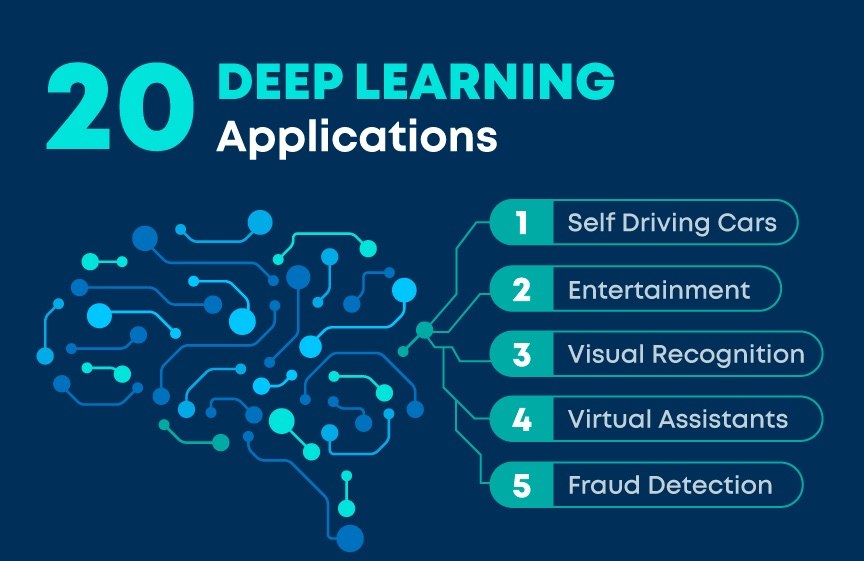
\includegraphics[width=\textwidth]{application_1.jpg}
                    \end{figure}
                \end{column}
                \begin{column}{0.5\textwidth}
                    \begin{figure}[H]
                          \centering
                          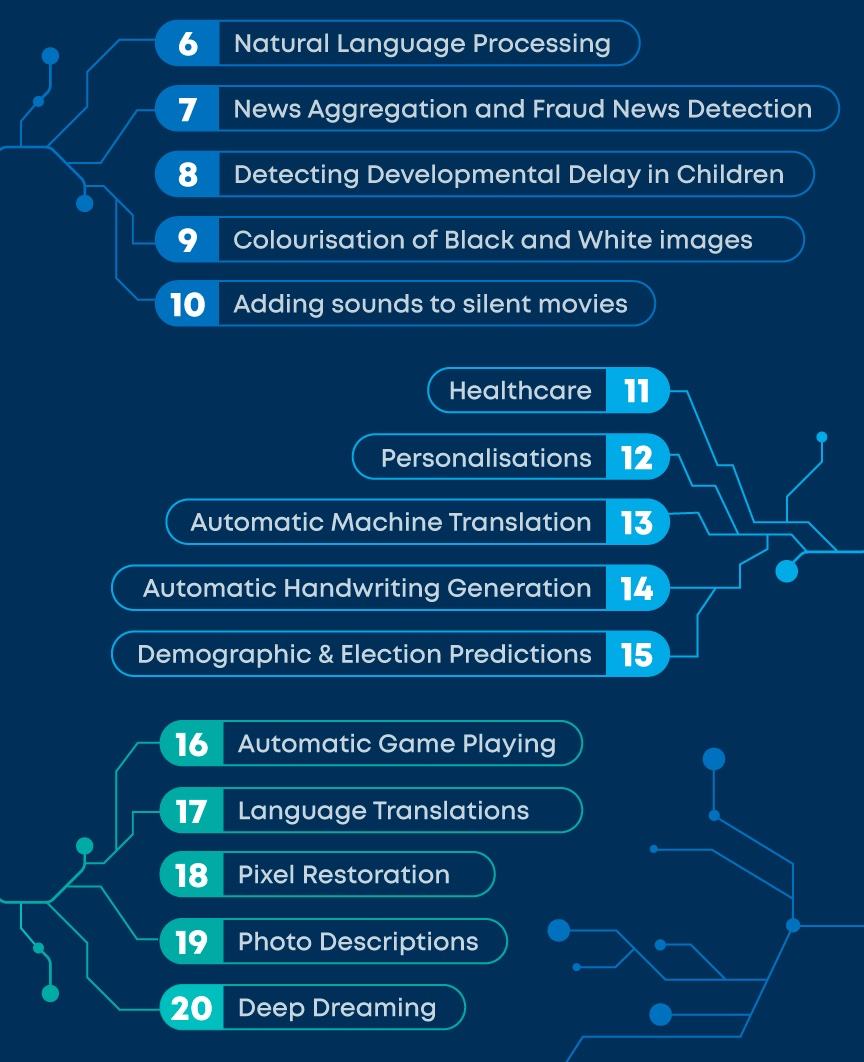
\includegraphics[width=\textwidth]{application_2.jpg}
                          \label{fig:pic1_1}
                    \end{figure}
                \end{column}
            \end{columns}
            %     \item необходимость обучать модели на больших массивах данных, что часто невозможно, ввиду отсутствия необходимых технических средств
            %     \item необходимость в совершенствовании самих методов обучения таких моделей
            % \end{itemize}
        \end{frame}

        \begin{frame}{Актуальность (2)}
            К сожалению, в настоящее время одним из основных подходов при обучении глубоких нейросетей является использование зарекомендовавших себя методов при повышенных требованиях к количеству обучающих данных, что приводит к невозможности обучения таких моделей при аппаратных ограничениях. Тем не менее сложность самих моделей продолжает расти.

            \begin{itemize}
                \item AlexNet
                \item VGG16
                \item ResNet-50
                \item NASNet
                \item SENet
            \end{itemize}
            % \begin{figure}[H]
            %     \centering                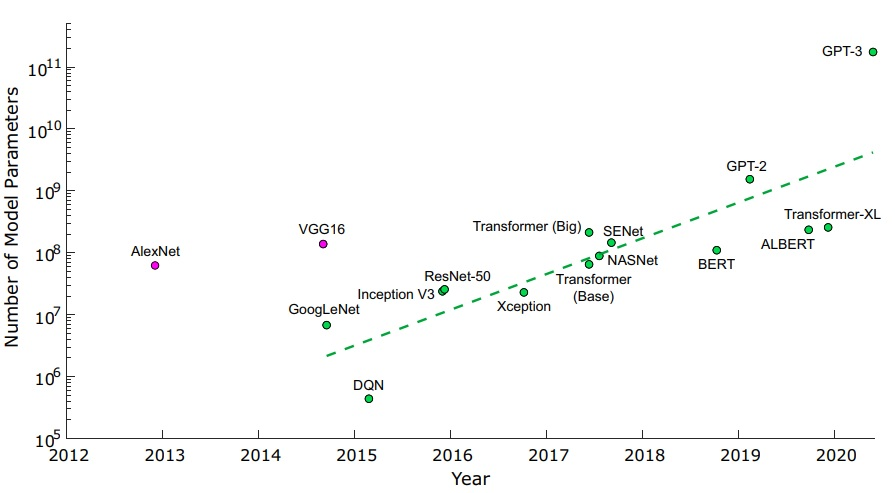
\includegraphics[width=0.95\textwidth]{pic_0.jpg}
            % \end{figure}
        \end{frame}

        \begin{frame}{Объект и предмет исследований}
            \begin{block}{Цель}
                \large
                Разработка \textbf{эффективных методов и алгоритмов} для обучения глубоких нейронных сетей, используемых для решения \textbf{задач компьютерного зрения}, включающих \textbf{распознавание маркировки продукции} на конвейерной линии и \textbf{определение наличия солнечных панелей} на аэрофотоснимках.
            \end{block}

            \begin{block}{Объект исследований}
                Нейросетевые системы компьютерного зрения
            \end{block}

            \begin{block}{Предмет исследований}
                Методы и алгоритмы обучения глубоких нейронных сетей и их применение к задачам компьютерного зрения
            \end{block}
        \end{frame}

        % \begin{frame}{Научная новизна}
        %     Научная новизна состоит в выявлении и доказательстве эквивалентности максимизации функции правдоподобия распределения входных данных в пространстве синаптических связей ограниченной машины Больцмана и минимизации кросс-энтропии функции ошибки сети, а также суммарной квадратичной ошибки сети при использовании линейных нейронов.\par

        %     Разработаны методы неконтролируемого предобучения глубоких нейронных сетей на базе доказанных эквивалентностей, что позволяет учитывать нелинейную природу нейронных элементов в процессе обучения.\par

        %     Разработан метод сокращения параметров нейросетевой модели, основывающийся на методе предобучения и позволяющий уменьшить количество настраиваемых параметров полносвязных и сверточных нейронных сетей без потери обобщающей способности.\par

        %     Разработаны нейросетевые системы компьютерного зрения (система распознавания маркировки на производственной линии, система обнаружения солнечных панелей на аэрофотоснимках), которые основываются на применении предложенного метода для выполнения предобучения соответствующих нейросетевых моделей.
        % \end{frame} 

        \begin{frame}{Методы обучения ГНС}
            \begin{figure}[H]
                  \centering
                  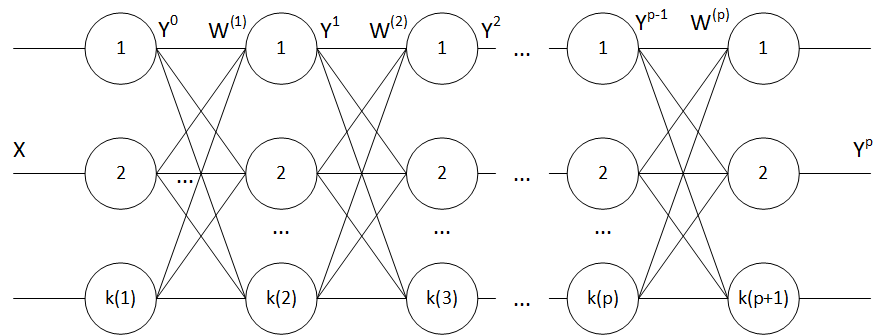
\includegraphics[width=0.8\textwidth]{pic1-1.png}
            \end{figure}
            Методы обучения ГНС используют предварительное обучениe (предобучение) в качестве этапа инициализирующей настройки параметров модели
            \begin{columns}
                \begin{column}{0.55\textwidth}
                    \begin{enumerate}
                        \item I тип -- С использованием предобучения на большой обучающей выборке;
                        \item II тип -- С использованием \textit{неконтролируемого} предобучения.
                    \end{enumerate}
                \end{column}
                \begin{column}{0.45\textwidth}
                    \begin{figure}[H]
                        \centering
                        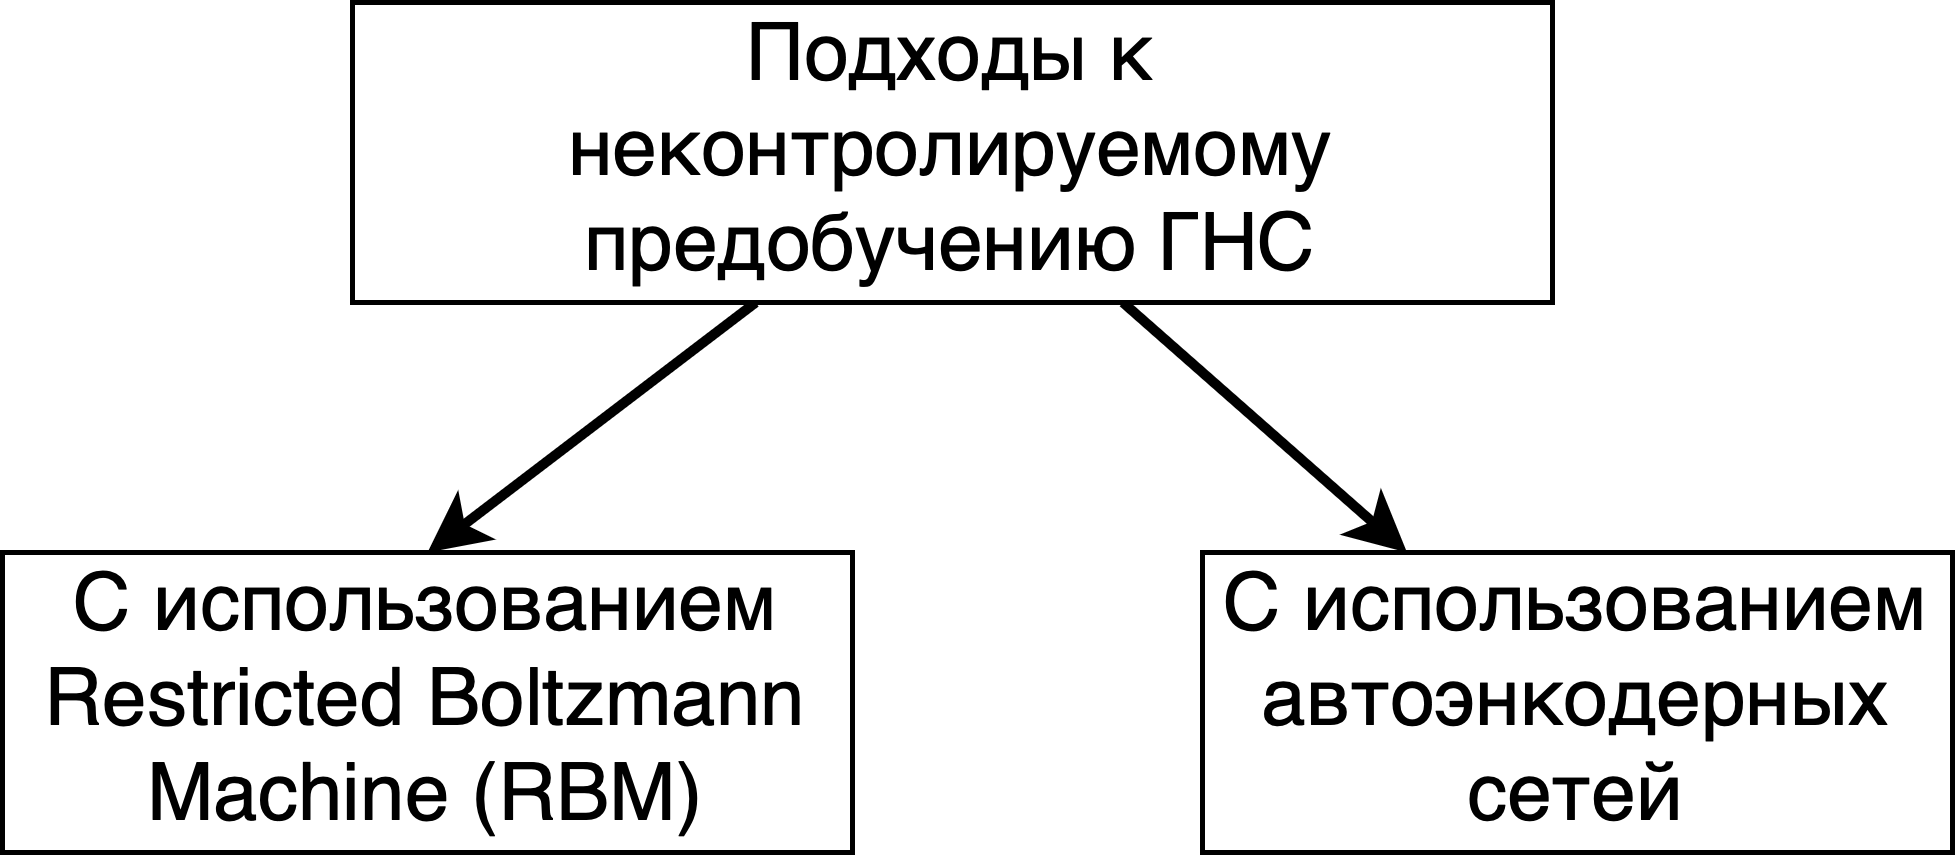
\includegraphics[width=1\textwidth]{pretrain_approaches.png}
                    \end{figure}
                \end{column}
            \end{columns}
        \end{frame}

        \begin{frame}{Обучение с использованием неконтролируемого предобучения на основе RBM}
            \begin{columns}
                \begin{column}{0.5\textwidth}
                    \begin{figure}[H]
                        \centering
                        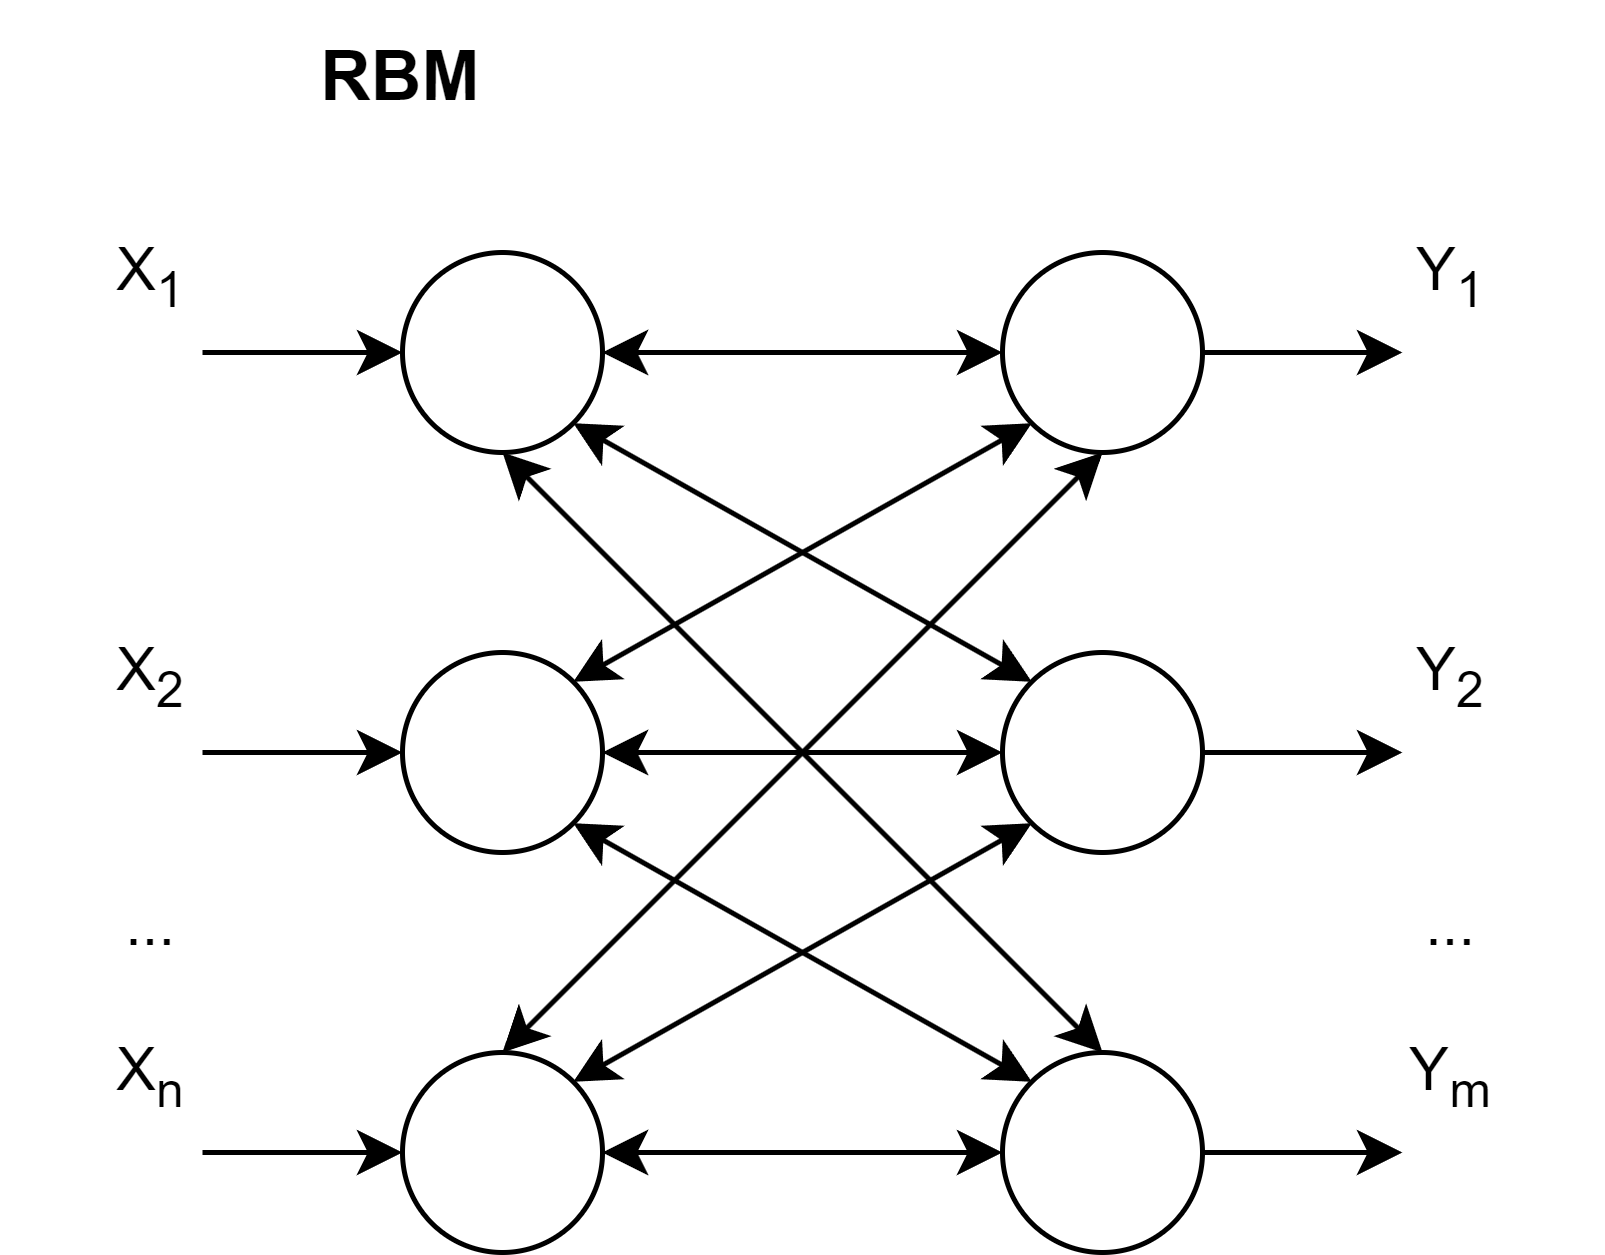
\includegraphics[width=0.8\textwidth]{pic1-3.png}
                    \end{figure}
                    \underline{Этапы обучения}:
                    \begin{enumerate}
                        \item Послойное неконтролируемое предобучение нейронной сети;
                        \item Настройка синаптических связей всей сети (<<доводка>> параметров);
                    \end{enumerate}
                \end{column}
                \begin{column}{0.5\textwidth}
                    \centering
                    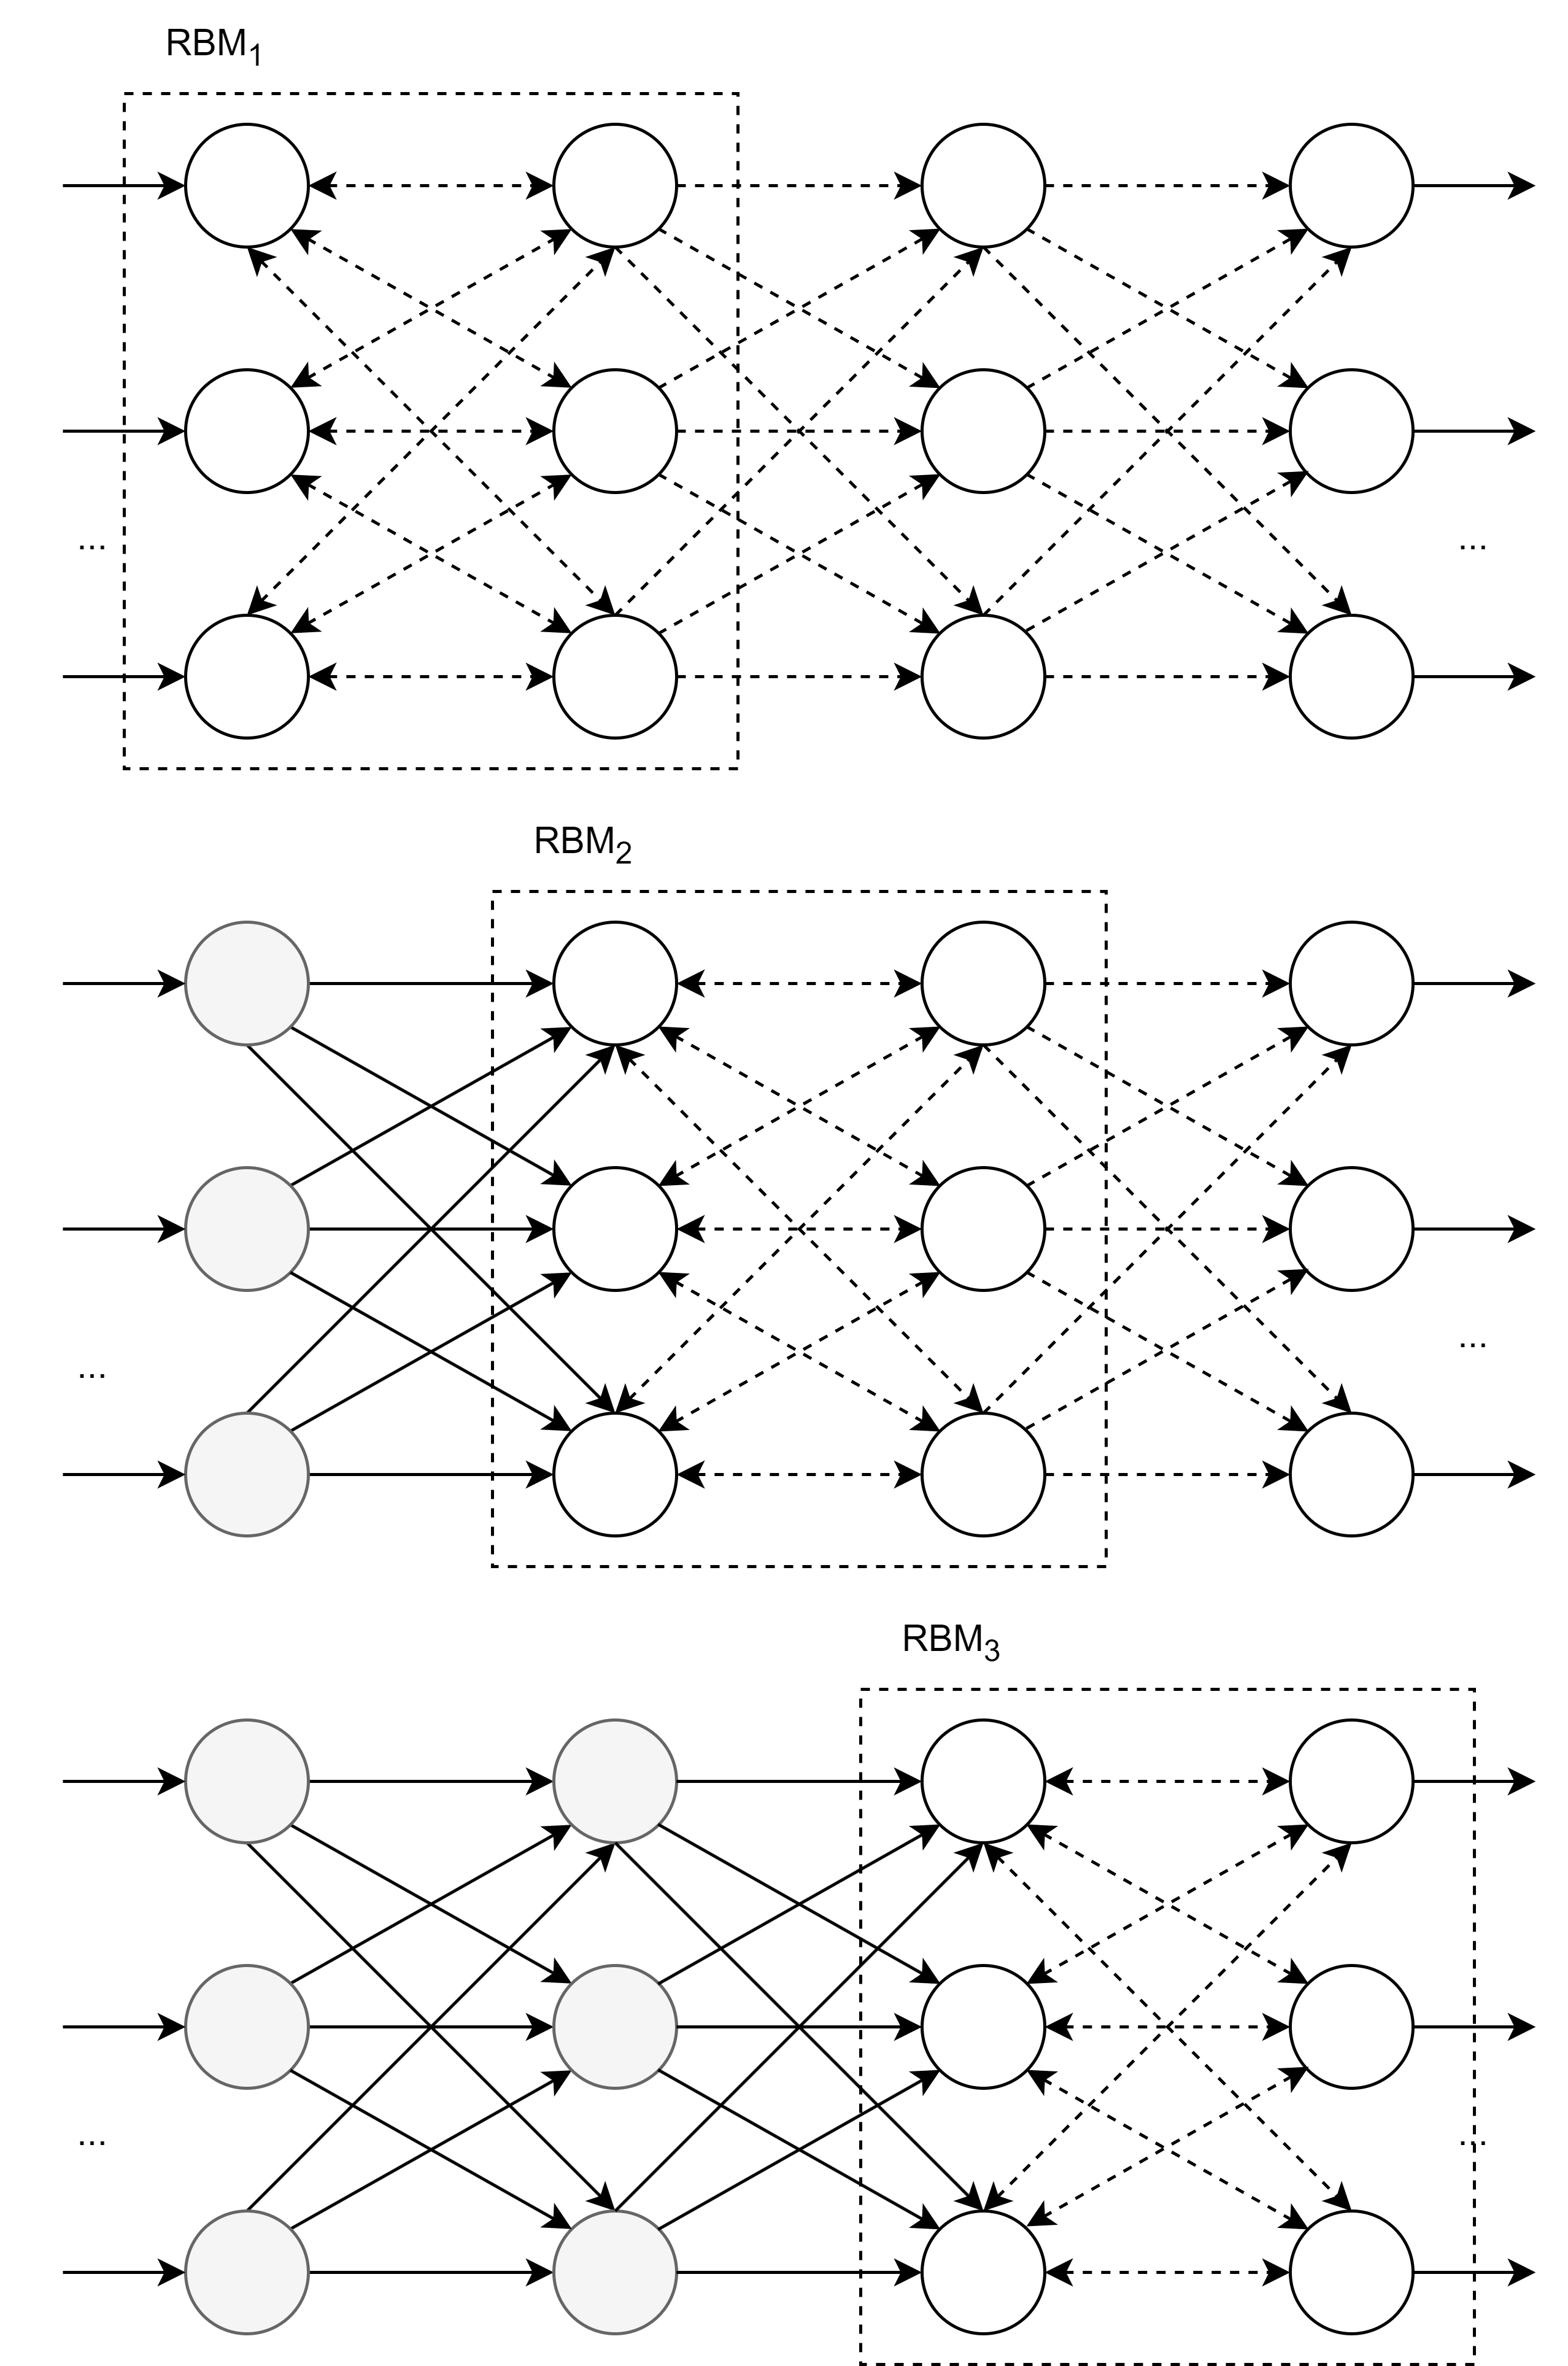
\includegraphics[width=0.8\textwidth]{full_network_training.png}
                \end{column}
            \end{columns}
        \end{frame}

        \begin{frame}{Обучение RBM}
            \begin{columns}
                \begin{column}{0.4\textwidth}
                    \begin{figure}[H]
                        \centering
                        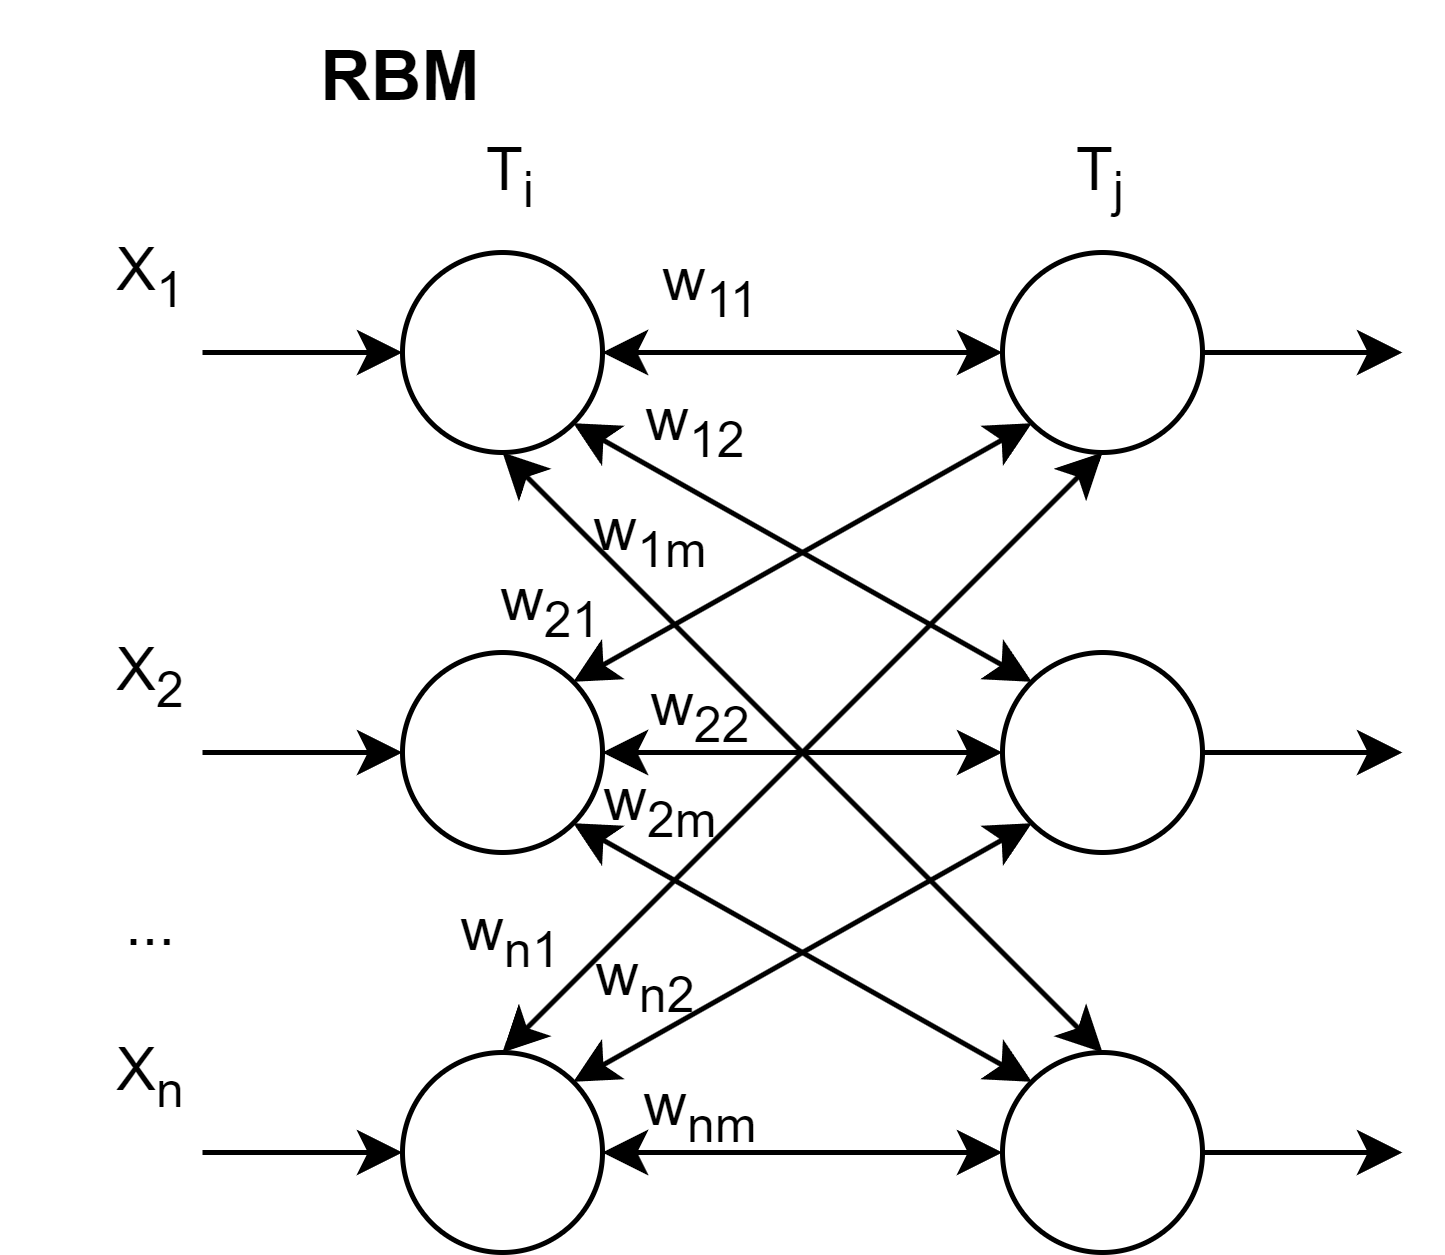
\includegraphics[width=0.9\textwidth]{pic4.png}
                        \label{fig:pic1_2}
                    \end{figure}
                \end{column}
                \begin{column}{0.6\textwidth}
                    \begin{equation*}
	                   \ln P(x)=\ln \sum_y e^{-E(x,y)}-\ln \sum_{x,y} e^{-E(x,y)}
                    \end{equation*}
                    Обучение в процессе реализации процедуры CD (Contrastive Divergence):
                    \begin{multline*}
	                   x(0) \rightarrow y(0) \rightarrow x(1) \rightarrow y(1) \rightarrow \ldots \\ \rightarrow x(k) \rightarrow y(k)
                    \end{multline*}
                \end{column}
            \end{columns}
            \underline{Правила обучения (случай CD-k)}
            \begin{equation*}
		    w_{ij}(t+1)=w_{ij}(t)+\alpha(x_i(0)y_j(0)-x_i(k)y_j(k))
            \end{equation*}
            \begin{equation*}		
		        T_i(t+1)=T_i(t)+\alpha(x_i(0)-x_i(k))
            \end{equation*}
            \begin{equation*}		
		        T_j(t+1)=T_j(t)+\alpha(y_j(0)-y_j(k)).
            \end{equation*}	
        \end{frame}

        \begin{frame}{Положения, выносимые на защиту (1)}
            \begin{block}{1}
                \large
                \textbf{Установление эквивалентности} задач максимизации функции правдоподобия распределения входных данных, минимизации кросс-энтропийной функции ошибки и суммарной квадратичной ошибки при использовании линейных нейронов в пространстве синаптических связей ограниченной машины Больцмана, что позволяет учитывать нелинейную природу нейронных элементов.
            \end{block}
        \end{frame}

        \begin{frame}{Альтернативное представление RBM (1)}
            \begin{figure}[H]
                \centering
                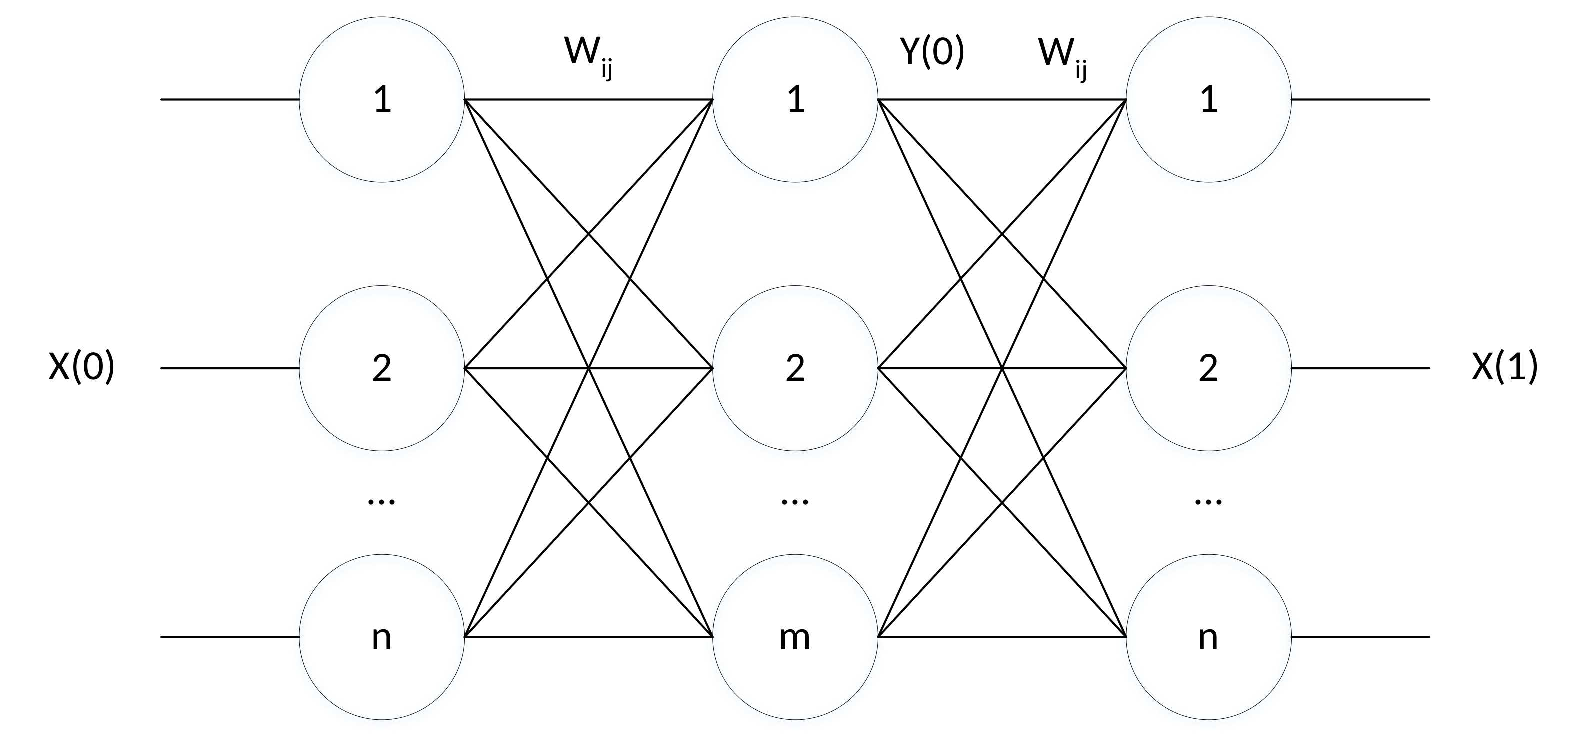
\includegraphics[width=0.8\textwidth]{pic2-1.pdf}
            \end{figure}
            \begin{center}
                \begin{tabular}{c|c}
                    $S_j(0)=\sum_i w_{ij}x_i(0)+T_j$ & $S_i(1)=\sum_j w_{ij}y_j(0)+T_i$ \\
                    $y_j(0)=F(S_j(0))$ &
                    $x_i(1)=F(S_i(1))$
                    \\
                    \hline
                    ... & ...\\
                    \hline
                    $S_i(k)=\sum_j w_{ij}y_j(k-1)+T_i$ & $S_j(k)=\sum_i w_{ij}x_i(k)+T_j$ \\
                    $x_i(k)=F(S_i(k))$ &
                    $y_j(k)=F(S_j(k))$
                \end{tabular}
            \end{center}
        \end{frame}

        \begin{frame}{Критерии минимизации}
            \begin{equation*}	
                E_s(k)=\frac{1}{2L}\Bigg(\sum_{l=1}^L\sum_{j=1}^m\sum_{p=1}^k (y_j^l(p)-y_j^l(p-1))^2+\sum_{l=1}^L\sum_{i=1}^n\sum_{p=1}^k (x_i^l(p)-x_i^l(p-1))^2\Bigg)
            \end{equation*}

            \begin{equation*}
	           CE_v(k) = -\frac{1}{L}\sum_{l=1}^L \sum_{p=1}^k \sum_{i=1}^n x_i^l(p-1)\log(x_i^l(p))+(1-x_i^l(p-1)\log(1-x_i^l(p))
            \end{equation*}

            \begin{equation*}
	           CE_h(k) = -\frac{1}{L}\sum_{l=1}^L \sum_{p=1}^k \sum_{j=1}^m y_j^l(p-1)\log(y_j^l(p))+(1-y_j^l(p-1)\log(1-y_j^l(p))
            \end{equation*}

            \begin{equation*}
	       CE_s(k) = CE_h(k)+CE_v(k)
            \end{equation*}
        \end{frame}

        \begin{frame}{Теоремы об эквивалентности}
            \begin{block}{}
                \textbf{Теорема 1}. Максимизация функции правдоподобия распределения данных $P(x)$ в пространстве синаптических связей ограниченной машины Больцмана эквивалентна минимизации суммарной квадратичной ошибки сети в том же пространстве при использовании линейных нейронов.
            \end{block}

            \begin{block}{}
                \textbf{Теорема 4}. Максимизация функции правдоподобия распределения входных данных $P(x)$ эквивалентна минимизации кросс-энтропийной целевой функции $CE_s(k)$ в одном и том же пространстве синаптических весов ограниченной машины Больцмана.
            \end{block}

            \begin{block}{}
                \textbf{Теорема 5}. Максимизация функции правдоподобия распределения входных данных $P(x)$ эквивалентна минимизации кросс-энтропийной функции и специальному случаю минимизации среднеквадратичной ошибки в одном и том же пространстве синаптических весов ограниченной машины Больцмана:
    
                \begin{equation*}
                	\max(\ln P(x)) = \min(CE_s) = \min(E_s)
                \end{equation*}
            \end{block}
        \end{frame}

        \begin{frame}{Положения, выносимые на защиту (2)}
            \begin{block}{2}
                \large
                \textbf{Метод обучения ограниченной машины Больцмана}, базирующийся на эквивалентности задач максимизации функции правдоподобия распределения входных данных и минимизации суммарной квадратичной ошибки при использовании линейных нейронов в пространстве синаптических связей сети, что позволяет \textbf{расширить класс обучаемых моделей и повысить обобщающую способность глубоких нейронных сетей}.
            \end{block}
        \end{frame}

        \begin{frame}{Метод обучения RBM: последовательное обучение}
            \underline{Случай CD-\textit{1}}:
            \begin{equation*}
                w_{ij}(t+1)=w_{ij}(t)-\alpha((y_j(1)-y_j(0))F'(S_j(1))x_i(1)+(x_i(1)-x_i(0))F'(S_i(1))y_j(0)),
            \end{equation*}

            \begin{equation*}
                T_i(t+1)=T_i(t)-\alpha(x_i(1)-x_i(0))F'(S_i(1)),
            \end{equation*}

            \begin{equation*}
                T_j(t+1)=T_j(t)-\alpha(y_j(1)-y_j(0))F'(S_j(1)).  
            \end{equation*}
            
            \underline{Случай CD-\textit{k}}:
            \begin{multline*}
                w_{ij}(t+1)=w_{ij}(t)-\\-\alpha\Bigg(\sum_{p=1}^k (y_j(p)-y_j(p-1))x_i(p)F'(S_j(p))+(x_i(p)-x_i(p-1))y_j(p-1)F'(S_i(p))\Bigg)
            \end{multline*}

            \begin{equation*}
            \begin{aligned}
                T_i(t+1)=T_i(t)-\alpha\left(\sum_{p=1}^k (x_i(p)-x_i(p-1))F'(S_i(p))\right),\\
                T_j(t+1)=T_j(t)-\alpha\left(\sum_{p=1}^k (y_j(p)-y_j(p-1))F'(S_j(p))\right),
            \end{aligned}
            \end{equation*}
        \end{frame}

        \begin{frame}{Метод обучения RBM: групповое обучение (1)}
            \underline{Случай CD-\textit{1}}:
            \begin{multline*}
                w_{ij}(t+1)=w_{ij}(t)-\\-\frac{\alpha}{L}\left(\sum_{l=1}^L (y_j^l(1)-y_j^l(0))x_i^l(1)F'(S_j^l(1))+(x_i^l(1)-x_i^l(0))y_j^l(0)F'(S_i^l(1))\Bigg)\right.,
            \end{multline*}

            \begin{equation*}
                T_i(t+1)=T_i(t)-\frac{\alpha}{L}\left(\sum_{l=1}^L (x_i^l(1)-x_i^l(0))F'(S_i^l(1))\right),
            \end{equation*}

            \begin{equation*}
                T_j(t+1)=T_j(t)-\frac{\alpha}{L}\left(\sum_{l=1}^L (y_j^l(1)-y_j^l(0))F'(S_j^l(1))\right)
            \end{equation*}
        \end{frame}

        \begin{frame}{Метод обучения RBM: групповое обучение (2)}
            \underline{Случай CD-\textit{k}}:
            \begin{multline*}
                w_{ij}(t+1)=w_{ij}(t)-\\-\frac{\alpha}{L}\Bigg(\sum_{l=1}^L\sum_{p=1}^k (y_j^l(p)-y_j^l(p-1))x_i^l(p)F'(S_j^l(p))+(x_i^l(p)-x_i^l(p-1))y_j^l(p-1)F'(S_i^l(p))\Bigg),
            \end{multline*}

            \begin{equation*}
                T_{i}(t+1)=T_{i}(t)-\frac{\alpha}{L}\left(\sum_{l=1}^L\sum_{p=1}^k (x_i^l(p)-x_i^l(p-1))F'(S_i^l(p))\right),
            \end{equation*}

            \begin{equation*}
                T_{j}(t+1)=T_{j}(t)-\frac{\alpha}{L}\left(\sum_{l=1}^L\sum_{p=1}^k (y_j^l(p)-y_j^l(p-1))F'(S_j^l(p))\right)
            \end{equation*}
        \end{frame}

        \begin{frame}{Метод обучения CRBM: последовательное обучение}
            \underline{Случай CD-\textit{1}}:
            \begin{multline*}
                w_{ij}(t+1)=w_{ij}(t)-\alpha((y_j(1)-y_j(0))F'(S_j(1))\circledast x_i(1)+\\(x_i(1)-x_i(0))F'(S_i(1))\circledast y_j(0)),    
            \end{multline*}
            \begin{equation*}
                T_i(t+1)=T_i(t)-\alpha(x_i(1)-x_i(0))F'(S_i(1)),
            \end{equation*}
            \begin{equation*}
                T_j(t+1)=T_j(t)-\alpha(y_j(1)-y_j(0))F'(S_j(1)).  
            \end{equation*}

            \underline{Случай CD-\textit{k}}:
            \begin{multline*}
                w_{ij}(t+1)=w_{ij}(t)-\\-\alpha\Bigg(\sum_{p=1}^k (y_j(p)-y_j(p-1))F'(S_j(p)) \circledast x_i(p) +(x_i(p)-x_i(p-1))F'(S_i(p)) \circledast y_j(p-1)\Bigg)
            \end{multline*}

            \begin{equation*}
            \begin{aligned}
                T_i(t+1)=T_i(t)-\alpha\left(\sum_{p=1}^k (x_i(p)-x_i(p-1))F'(S_i(p))\right),\\
                T_j(t+1)=T_j(t)-\alpha\left(\sum_{p=1}^k (y_j(p)-y_j(p-1))F'(S_j(p))\right),
            \end{aligned}
            \end{equation*}
        \end{frame}

        \begin{frame}{Сравнение методов: используемые выборки}
        \begin{columns}
            \begin{column}{0.5\textwidth}
                \begin{figure}[H]
                    \centering
                    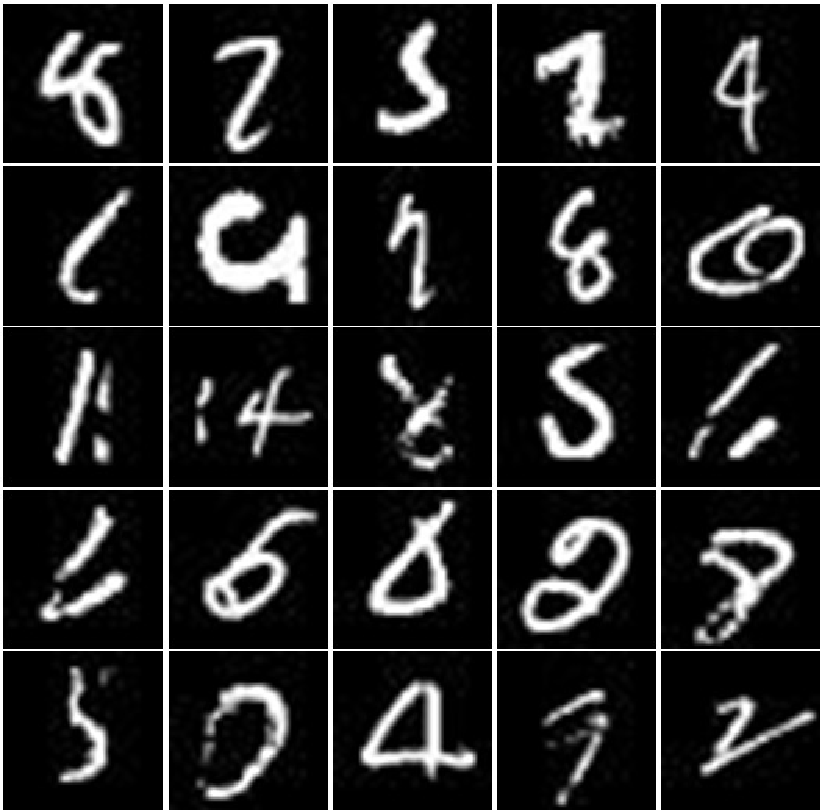
\includegraphics[width=0.6\textwidth]{pic3-12.pdf}
                \end{figure}
                \underline{Характеристики:}\\
                \textbf{MNIST}\\
                Количество классов: 10\\
                Обучающая часть: 50.000 из.\\
                Валидационная часть: 10.000 из.\\
                Размеры изображений: 28Х28\\
                Цветовая модель: Grayscale
            \end{column}
            
            \begin{column}{0.5\textwidth}
                \begin{figure}[H]
                    \centering
                    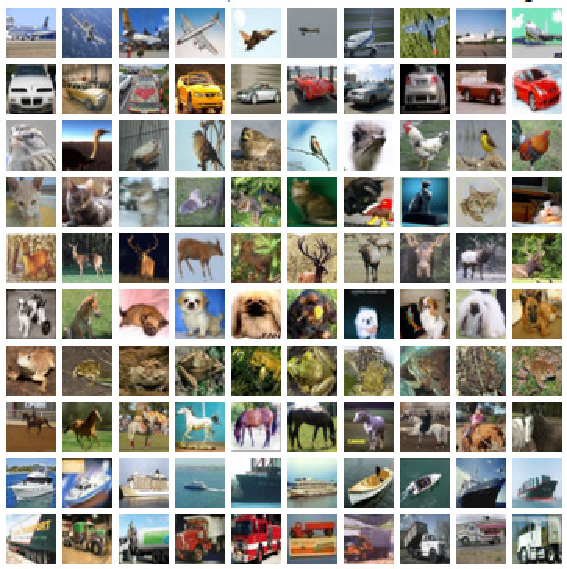
\includegraphics[width=0.6\textwidth]{pic3-2.pdf}
                \end{figure}
                \underline{Характеристики:}\\
                \textbf{CIFAR10/CIFAR100}\\
                Количество классов: 10/100\\
                Обучающая часть: 50.000 из.\\
                Валидационная часть: 10.000 из.\\
                Размеры изображений: 32Х32\\
                Цветовая модель: RGB
            \end{column}
        \end{columns}
        \end{frame}

        \begin{frame}{Используемое аппаратное и программное обеспечение}
            % Выполнение экспериментов с глубокими нейронными сетями даже при условии использования выборок среднего размера занимает продолжительное время и требует наличия значительных вычислительных ресурсов. Важными аппаратными ресурсами, влияющими на вычислительный процесс и потенциальными источниками аварийного завершения программы, становятся оперативная память и количество обрабатывающих элементов в случае использования графических ускорителей. В данной работе проблема наличия данных ресурсов была частично решена использованием сервиса Google Colab \cite{googlecolab}. Данный сервис предоставляет доступ к видеоускорителям A100 и V100, производительности которых оказалось достаточно для проведения всех расчетов. Существуют другие способы ускорения расчетов, производимых при обучении нейронной сети, например, использование вычислительных кластеров \cite[c.~701]{n16}. % проведением расчетов с использованием видеокарт nVidia, поддерживающих технологию CUDA (нами использовались ускорители A100 или V100, доступные при использовании сервиса Google Colab \cite{googlecolab}). Существуют другие способы ускорения расчетов, производимых при обучении нейронной сети, например, использование вычислительных кластеров \cite{n16}.
            \footnotesize
            % Также при обучении моделей использовались локальные ресурсы:
            \begin{columns}[T]
                \begin{column}[T]{0.5\textwidth}
                    \vspace{0pt}
                    \textbf{\underline{Аппаратное обеспечение:}}
                    \begin{itemize}
                        \item Google Colab;
                        \item ноутбук N580VD-DM298 (процессор Intel Core i7 7700HQ, 4-х ядерный, с максимальной тактовой частотой 3800 МГц; оперативная память 16 Гб типа DDR4; видеокарта NVIDIA GeForce GTX 1050 4 ГБ);
                        \item десктопный компьютер (процессор Intel Core i7-4790K, 4-х ядерный, с максимальной тактовой частотой 4.00 ГГц; оперативная память 8 Гб типа DDR3; видеокарта NVIDIA GeForce GTX 750 Ti 2 ГБ).
                    \end{itemize}
                    \textbf{\underline{Программное обеспечение:}}
                    \begin{itemize}
                        \item интерпретатор языка программирования Python версии 3.X.;
                        \item интегрированная среда разработки PyCharm;
                        \item Neptune -- пакет для поддержки эксперимента в области МО;
                    \end{itemize}
                \end{column}
                \begin{column}{0.5\textwidth}
                    \begin{itemize}
                        \item NumPy -- пакет для работы с массивами;
                        \item Pandas -- пакет для обработки и анализа данных;
                        \item Pillow -- пакет для работы с графическими файлами;
                        \item OpenCV -- библиотека для решения различных задач КЗ;
                        \item scikit-learn -- библиотека МО;
                        \item SciPy -- библиотека для научных и технических вычислений;
                        \item TensorFlow -- библиотека машинного обучения с акцентом на ГНС;
                        \item TensorBoard -- специализированная библиотека для визуализации и логирования обучения НС;
                        \item PyTorch -- библиотека МО с акцентом на ГНС, а также задачи CV и NLP;
                        \item Torchvision -- пакет, содержащий реализации основных архитектур моделей, применяемых при решении задач КЗ.
                    \end{itemize}
                \end{column}
            \end{columns}
            % В вычислительных экспериментах использовалось следующее основное программное обеспечение:
        \end{frame}

        \begin{frame}{Условные обозначения для исследуемых моделей}
            В данной работе используется следующая нотация для описания архитектур НС: 
            \begin{itemize}
                \item для полносвязных слоев \textit{N} x \textit{M}, где \textit{N} обозначает количество входных нейронов слоя, а \textit{M} -- количество выходных нейронов;  
                \item для сверточных слоев \textit{K} x \textit{S} x \textit{S}, где \textit{K} обозначает количество ядер свертки в соответствующем слое, a \textit{S} x \textit{S} -- размерность ядра свертки.
            \end{itemize}
            При этом для полносвязных слоев используется сокращенная форма нотации, обозначающая количество нейронов в каждом слое, например, нотация \textbf{784-100-100-10}, где 784 -- это число нейронов в первом (распределяющем) слое, 100 -- число нейронов во втором слое и так далее. 
        \end{frame}

        \begin{frame}{Сравнение методов (MNIST): параметры эксперимента}
            \underline{Параметры модели:}
            \begin{table}
            \small
            \begin{tabular}{|p{6cm}|p{5cm}|}
              \hline
                \textbf{Параметр} & \textbf{Значение}\\
                \hline
                Архитектура & 40Х5Х5 -- 40Х5Х5 -- 640Х320 -- 320Х160 -- 160Х10\\
                \hline
                Функция активации & ReLU \\
                \hline
                Функция активации на последнем слое & Softmax \\
                \hline
                Начальная инициализация параметров & Нормальное распредение \\
                \hline
                Общее число параметров модели & 299.170
                \\
                \hline
            \end{tabular}
            \end{table}\par
            \underline{Параметры обучения:}
            \begin{table}
            \small
            \begin{tabular}{|p{3cm}|p{5cm}|p{2cm}|}
              \hline
                \textbf{Этап} & \textbf{Параметр} & \textbf{Значение}\\
                \hline
                Предобучение & Скорость обучения & 0,000125\\
                \cline{2-3}
                & Размер мини-батча & 128 \\
                \cline{2-3}
                & Моментный параметр & [0,5; 0,9] \\
                \cline{2-3}
                & Количество эпох обучения & 30\\
                \hline
                Обучение & Скорость обучения & 0,001\\
                \cline{2-3}
                & Размер мини-батча & 128 \\
                \cline{2-3}
                & Моментный параметр & 0,9 \\
                \cline{2-3}
                & Количество эпох обучения & 50\\
                \hline
            \end{tabular}
            \end{table}
        \end{frame}

        \begin{frame}{Сравнение методов (MNIST): результаты}
            \begin{table} [!h]
              \small
            \centering
            \begin{tabular}{| p{3cm} | p{3cm} |}
              \hline
                \textbf{Метод обучения} & \textbf{Эффективность, \%}\\
                \hline
                BP & 99.367\\
                \hline
                REBA & 99.371\\
                \hline
                HREBA & \textbf{99.458}\\
                \hline
                C-RBM & 99.447\\
                \hline
            \end{tabular}
            \end{table}
            \begin{itemize}
                \item BP -- обучение без предобучения; 
                \item REBA -- обучение с предобучением (предлагаемый подход); 
                \item HREBA -- обучение с предобучением (гибридный подход);
                \item C-RBM -- обучение с классическим методом предобучения).
            \end{itemize}
            Лучший результат: \textbf{99.53} (HREBA)\\
            
            При обучении с помощью гибридного метода первый слой глубокой нейронной сети обучался как RBM с использованием классического метода обучения, а все последующие обучались предложенным методом.
        \end{frame}

        \begin{frame}{Сравнение методов (CIFAR10): параметры эксперимента}
            \underline{Параметры модели:}
            \begin{table}
            \small
            \begin{tabular}{|p{6cm}|p{5cm}|}
              \hline
                \textbf{Параметр} & \textbf{Значение}\\
                \hline
                Архитектура & 64Х5Х5 -- 32Х5Х5 -- 800Х128 -- 128Х10 / 128X100\\
                \hline
                Функция активации & ReLU - Tanh - ReLU \\
                \hline
                Функция активации на последнем слое & Softmax \\
                \hline
                Начальная инициализация параметров & Нормальное распредение \\
                \hline
                Общее число параметров модели & 159.914
                \\
                \hline
            \end{tabular}
            \end{table}\par
            \underline{Параметры обучения:}
            \begin{table}
            \small
            \begin{tabular}{|p{3cm}|p{5cm}|p{2cm}|}
              \hline
                \textbf{Этап} & \textbf{Параметр} & \textbf{Значение}\\
                \hline
                Предобучение & Скорость обучения & 0,000125\\
                \cline{2-3}
                & Размер мини-батча & 128 \\
                \cline{2-3}
                & Моментный параметр & [0,5; 0,9] \\
                \cline{2-3}
                & Количество эпох обучения & 30\\
                \hline
                Обучение & Скорость обучения & 0,001\\
                \cline{2-3}
                & Размер мини-батча & 128 \\
                \cline{2-3}
                & Моментный параметр & 0,9 \\
                \cline{2-3}
                & Количество эпох обучения & 25\\
                \hline
            \end{tabular}
            \end{table}
        \end{frame}

        \begin{frame}{Сравнение методов (CIFAR10): результаты}
            \begin{table} [!h]
              \small
            \centering
            \begin{tabular}{| p{3cm} | p{3cm} |}
              \hline
                \textbf{Метод обучения} & \textbf{Эффективность, \%}\\
                \hline
                BP & 69.74\\
                \hline
                REBA & 71.20\\
                \hline
                HREBA & \textbf{71.59}\\
                \hline
                C-RBM & 71.51\\
                \hline
            \end{tabular}
            \end{table}
            \begin{itemize}
                \item BP -- обучение без предобучения; 
                \item REBA -- обучение с предобучением (предлагаемый подход); 
                \item HREBA -- обучение с предобучением (гибридный подход);
                \item C-RBM -- обучение с классическим методом предобучения).
            \end{itemize}
            Лучший результат: \textbf{72.32} (HREBA)\\

            % Несмотря на в целом неплохой результат, полученный с помощью метода без предобучения, наблюдается постепенная деградация обучения с увеличением глубины модели.
        \end{frame}

        \begin{frame}{Сравнение методов (CIFAR100): результаты}
            \begin{table} [!h]
              \small
            \centering
            \begin{tabular}{| p{3cm} | p{3cm} |}
              \hline
                \textbf{Метод обучения} & \textbf{Эффективность, \%}\\
                \hline
                BP & 36.83\\
                \hline
                REBA & 38.9\\
                \hline
                HREBA & \textbf{39.86}\\
                \hline
                C-RBM & 39.71\\
                \hline
            \end{tabular}
            \end{table}
            \begin{itemize}
                \item BP -- обучение без предобучения; 
                \item REBA -- обучение с предобучением (предлагаемый подход); 
                \item HREBA -- обучение с предобучением (гибридный подход);
                \item C-RBM -- обучение с классическим методом предобучения).
            \end{itemize}
            Лучший результат: \textbf{40.26} (HREBA)\\
        \end{frame}

        \begin{frame}{Положения, выносимые на защиту (3)}
            \begin{block}{3}
                \large
                \textbf{Алгоритм редуцирования параметров глубокой нейронной сети}, базирующийся на неконтролируемом предобучении сети, что позволяет упростить ее архитектуру (путем сокращения числа настраиваемых параметров модели) \textbf{без потери обобщающей способности}.
            \end{block}
        \end{frame}

        \begin{frame}{Алгоритм редуцирования параметров}
        \begin{columns}
            \begin{column}{0.6\textwidth}
            \begin{enumerate}
                \item Неконтролируемое предобучение НС, начиная с первого слоя;
                \item \textit{Обнуление} параметров НС, значения которых попадают в интервал $[-t, t]$ для заданного $t>0$;
                \item Архитектурная реконфигурация НС.\\
                    для каждого \textit{i}-того слоя НС, кроме первого и последнего:
                    \begin{itemize}
                        \item если $j$-тый вектор-столбец матрицы весовых коэффициентов $W_i$ нулевой, то удалить $j$-тый вектор-столбец из $W_i$ и удалить $j$-тую вектор-строку из $W_{i+1}$;
                        \item если $k$-тая вектор-строка матрицы весовых коэффициентов $W_i$ нулевая, то удалить $k$-тую вектор-строку из $W_i$ и удалить $k$-тый вектор-столбец из матрицы $W_{i-1}$;
                    \end{itemize}
                % , в ходе которой удаляются нейроны, не участвующие в формировании выходной активности сети (нейроны, имеющие нулевые векторы весовых коэффициентов или, в случае использования сверточных слоев, нейроны, имеющие нулевые ядра свертки);
                \item \textbf{Тонкая настройка} нередуцированных параметров НС.
            \end{enumerate}
            \end{column}
            \begin{column}{0.4\textwidth}
                \begin{figure}[H]
                    \centering
                    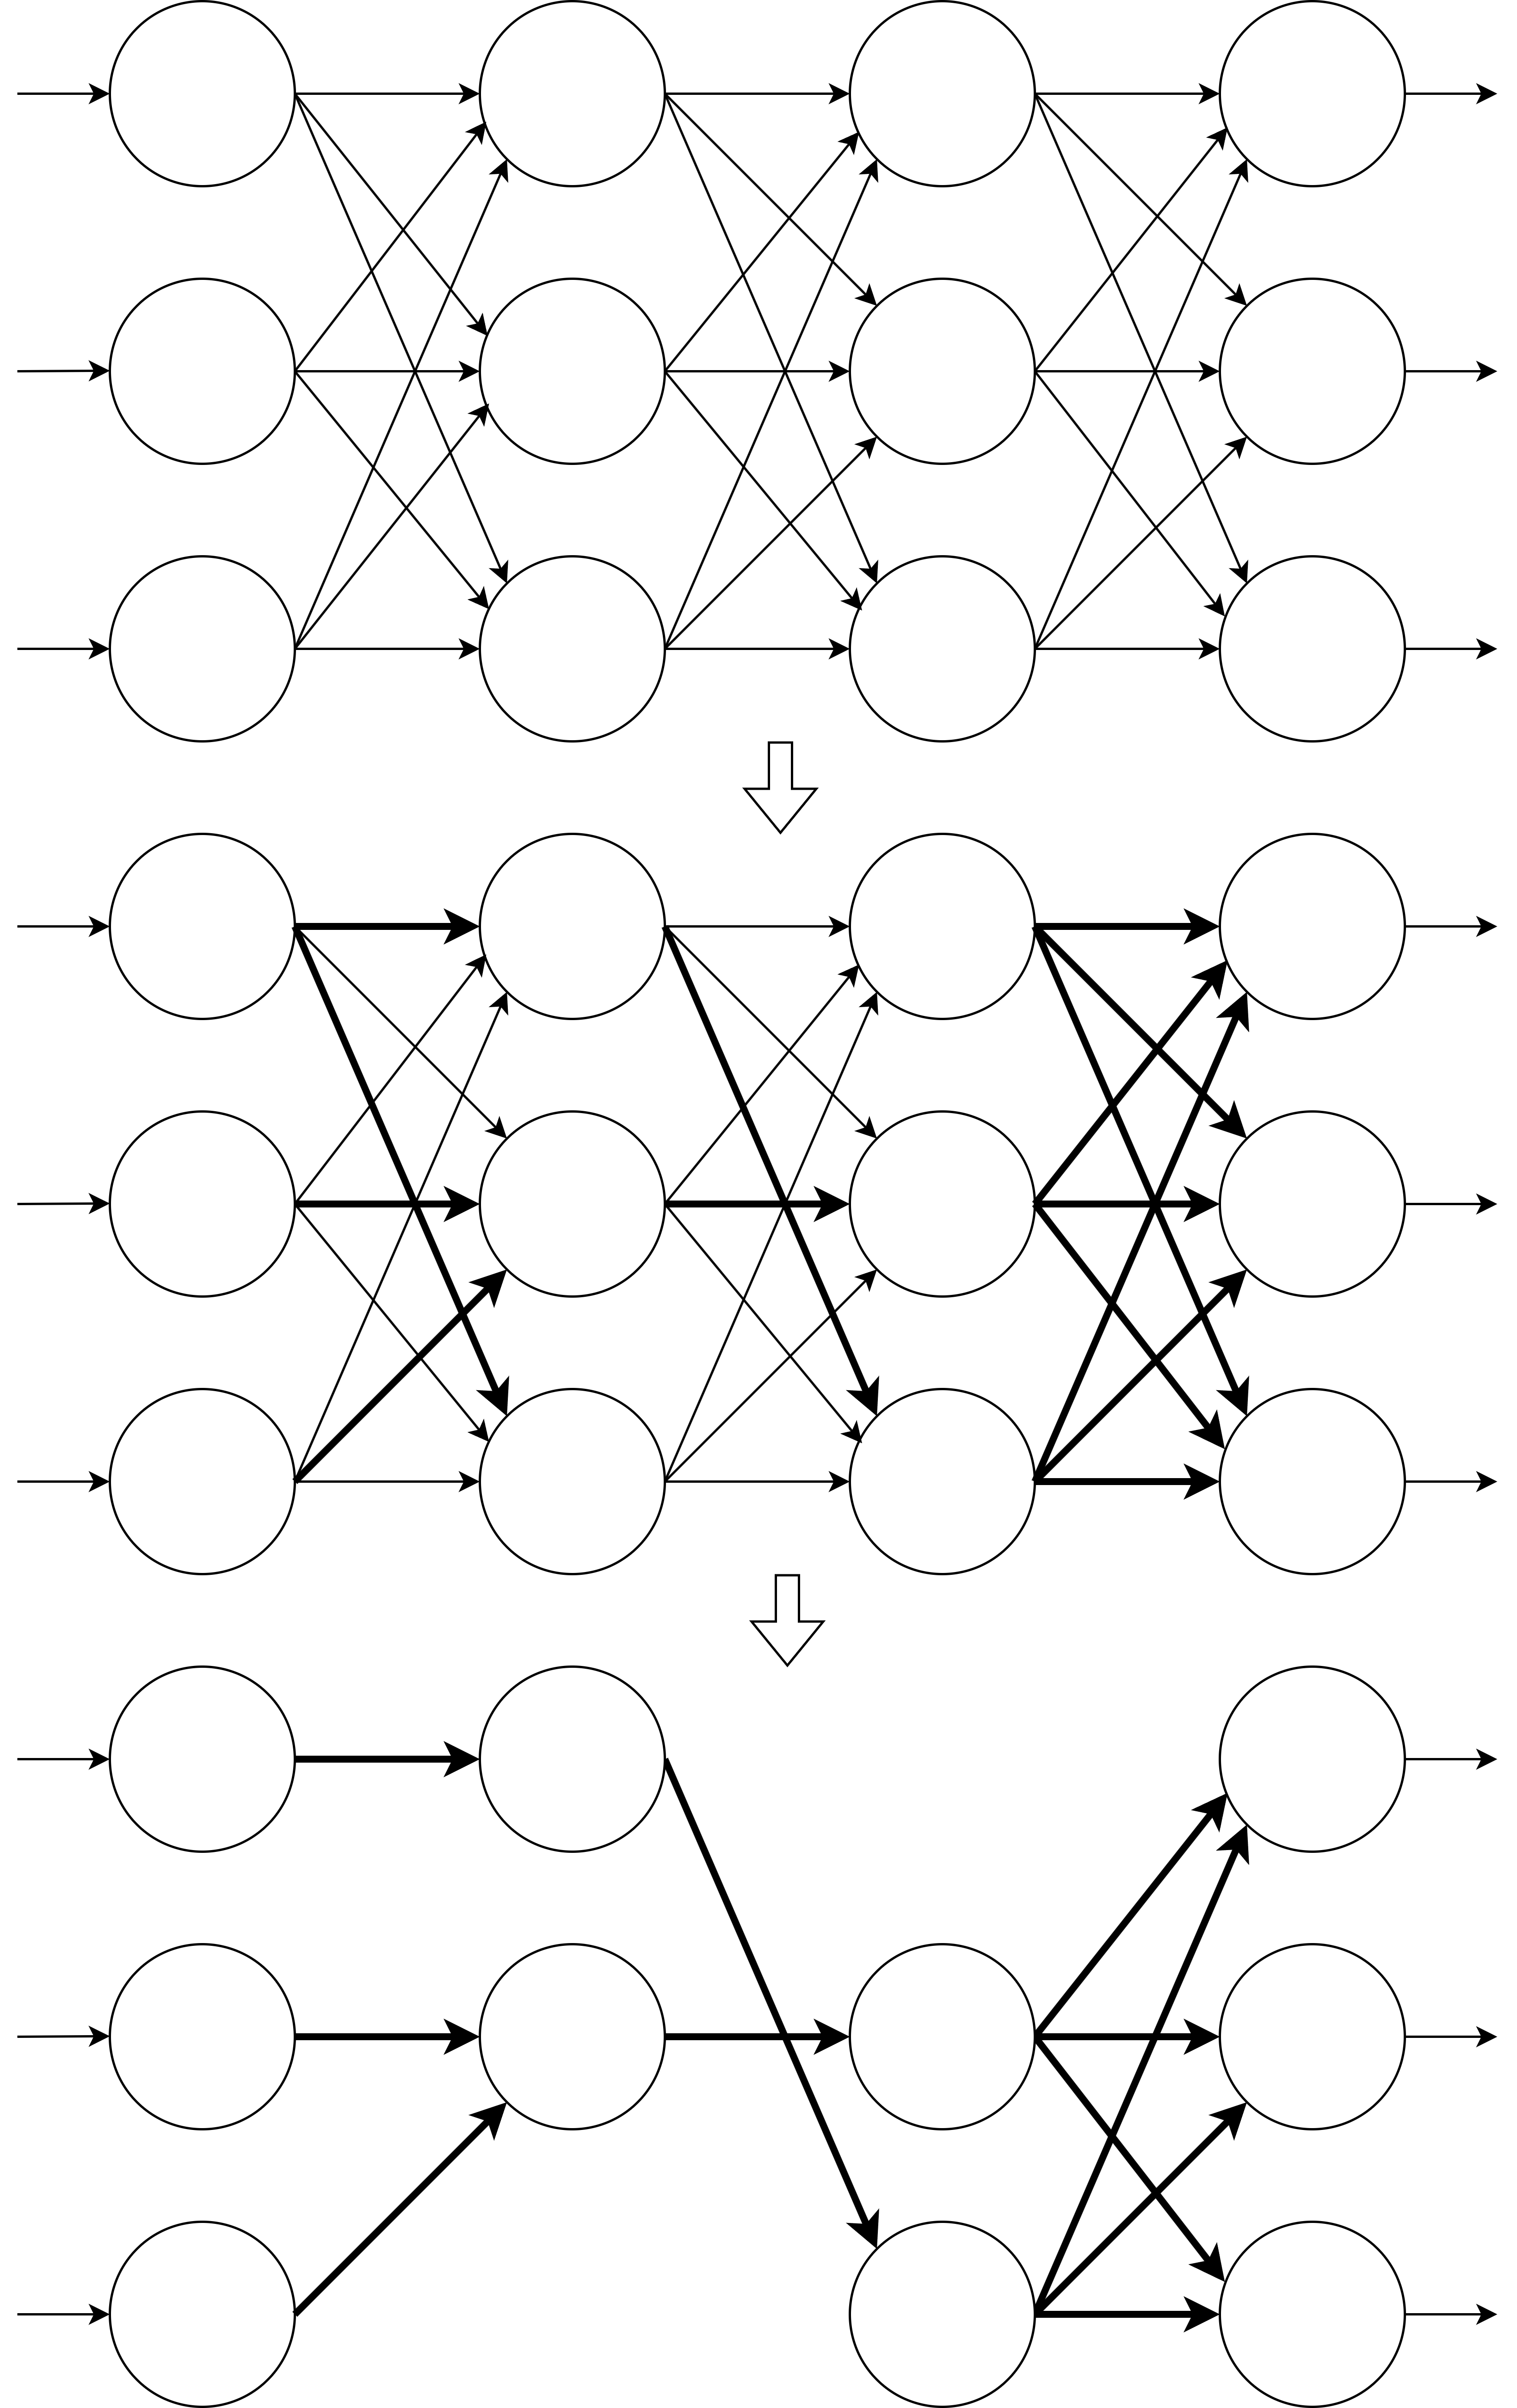
\includegraphics[width=01\textwidth]{pic2-3.png}
                \end{figure}
            \end{column}
        \end{columns}
        \end{frame}

        \begin{frame}{Алгоритм редуцирования: параметры эксперимента}
            \begin{table} [!h]
              \small
              \caption{Основные параметры обучения}\label{table:reduce_training_params}
            \centering
            \begin{tabular}{| p{2cm} | p{5cm} | p{2cm} |}
              \hline
                \textbf{Этап} & \textbf{Параметр} & \textbf{Значение}\\
                \hline
                Обучение & Скорость обучения & 0.05-0.1\\
                \cline{2-3}
                & Размер мини-батча & 100 \\
                \cline{2-3}
                & Моментный параметр & 0.9 \\
                \cline{2-3}
                & Количество эпох обучения & 50-100\\
                \hline
                Предобучение & Скорость обучения & 0.05-0.2\\
                \cline{2-3}
                & Размер мини-батча & 32-100 \\
                \cline{2-3}
                & Моментный параметр & [0.5, 0.9] \\
                \cline{2-3}
                & Количество эпох обучения & 10\\
                \hline
            \end{tabular}
            \end{table}
        \end{frame}

        \begin{frame}{Алгоритм редуцирования: результаты}
            \underline{784-800-800-10}
            \begin{table}
              \small
            \centering
            \begin{tabular}{| p{1.5cm} | p{2.5cm} | p{3cm} | p{2.5cm} |}
              \hline
                \textbf{Тип} & \textbf{Эффективность, \%, C-RBM / REBA} & \textbf{Количество параметров, C-RBM / REBA} & \textbf{Редуцировано параметров, \%, C-RBM / REBA}\\
                \hline
                без редуц. & \textbf{98.63} / 98.33 & 1276810 / 1276810 & 0/0\\
                \hline
                t=0.2 & \textbf{98.61} / 98.27 & \textbf{233760} / 279635 & \textbf{81.69} / 78.1\\
                \hline
                t=0.5 & 98.03 / \textbf{98.05} & \textbf{32524} / 32817 & \textbf{97.45} / 97.43\\
                \hline
                t=0.8 & \textbf{97.1} / 96.48 & 17061 / \textbf{12217} & 98.66 / \textbf{99.04}\\
                \hline
            \end{tabular}
            \end{table}

            \underline{784-1600-1600-800-800-10}
            \begin{table}
              \small
            \centering
            \begin{tabular}{| p{1.5cm} | p{2.5cm} | p{3cm} | p{2.5cm} |}
              \hline
                \textbf{Тип} & \textbf{Эффективность, \%, C-RBM / REBA} & \textbf{Количество параметров, C-RBM / REBA} & \textbf{Редуцировано параметров, \%, C-RBM / REBA}\\
                \hline
                без редуц. & \textbf{98.76} / 98.37 & 5747210 / 5747210 & 0/0\\
                \hline
                t=0.2 & 98.51 / \textbf{98.55} & \textbf{710734} / 781103 & \textbf{87.63} / 86.41\\
                \hline
                t=0.5 & 98.01 / \textbf{98.03} & 54709 / \textbf{43867} & 99.05 / \textbf{99.24}\\
                \hline
                t=0.8 & \textbf{96.9} / 93.08 & 25385 / \textbf{14914} & 99.56 / \textbf{99.74}\\
                \hline
            \end{tabular}
            \end{table}  
        \end{frame}

        \begin{frame}{Результаты архитектурной реконфигурации моделей}
            \underline{Исходная модель: 784-800-800-10}
            \begin{table} [!h]
              \small
                \centering
                \begin{tabular}{| p{2cm} | p{4cm} | p{4cm} |}
                \hline
                    \textbf{Параметр} & \textbf{Редуцированная}\\
                \hline
                t=0.2 & 784-800-556-10\\
                \hline
                t=0.5 & 784-710-422-10\\
                \hline
                t=0.9 & 784-91-114-10\\
                \hline
                \end{tabular}
                \end{table}

                \underline{Исходная модель: 784-1600-1600-800-800-10}
              \begin{table} [!h]
              \small
                \centering
                \begin{tabular}{| p{2cm} | p{4cm} | p{4cm} |}
                \hline
                    \textbf{Параметр} &  \textbf{Редуцированная}\\
                \hline
                t=0.2 & 784-889-192-686-221-10\\
                \hline
                t=0.5 & 784-464-157-567-182-10\\
                \hline
                t=0.9 & 784-17-101-118-50-10\\
                \hline
                \end{tabular}
            \end{table}
        \end{frame}

        \begin{frame}{Положения, выносимые на защиту (4)}
            \begin{block}{4}
                \large
                \textbf{Нейросетевая система компьютерного зрения}, основывающаяся на предлагаемом методе предобучения нейросетевых моделей, применение которой позволяет улучшить качество решения задач классификации. 
            \end{block}
        \end{frame}

        \begin{frame}{Архитектура разработанной системы}
            \begin{figure}[H]
                \centering
                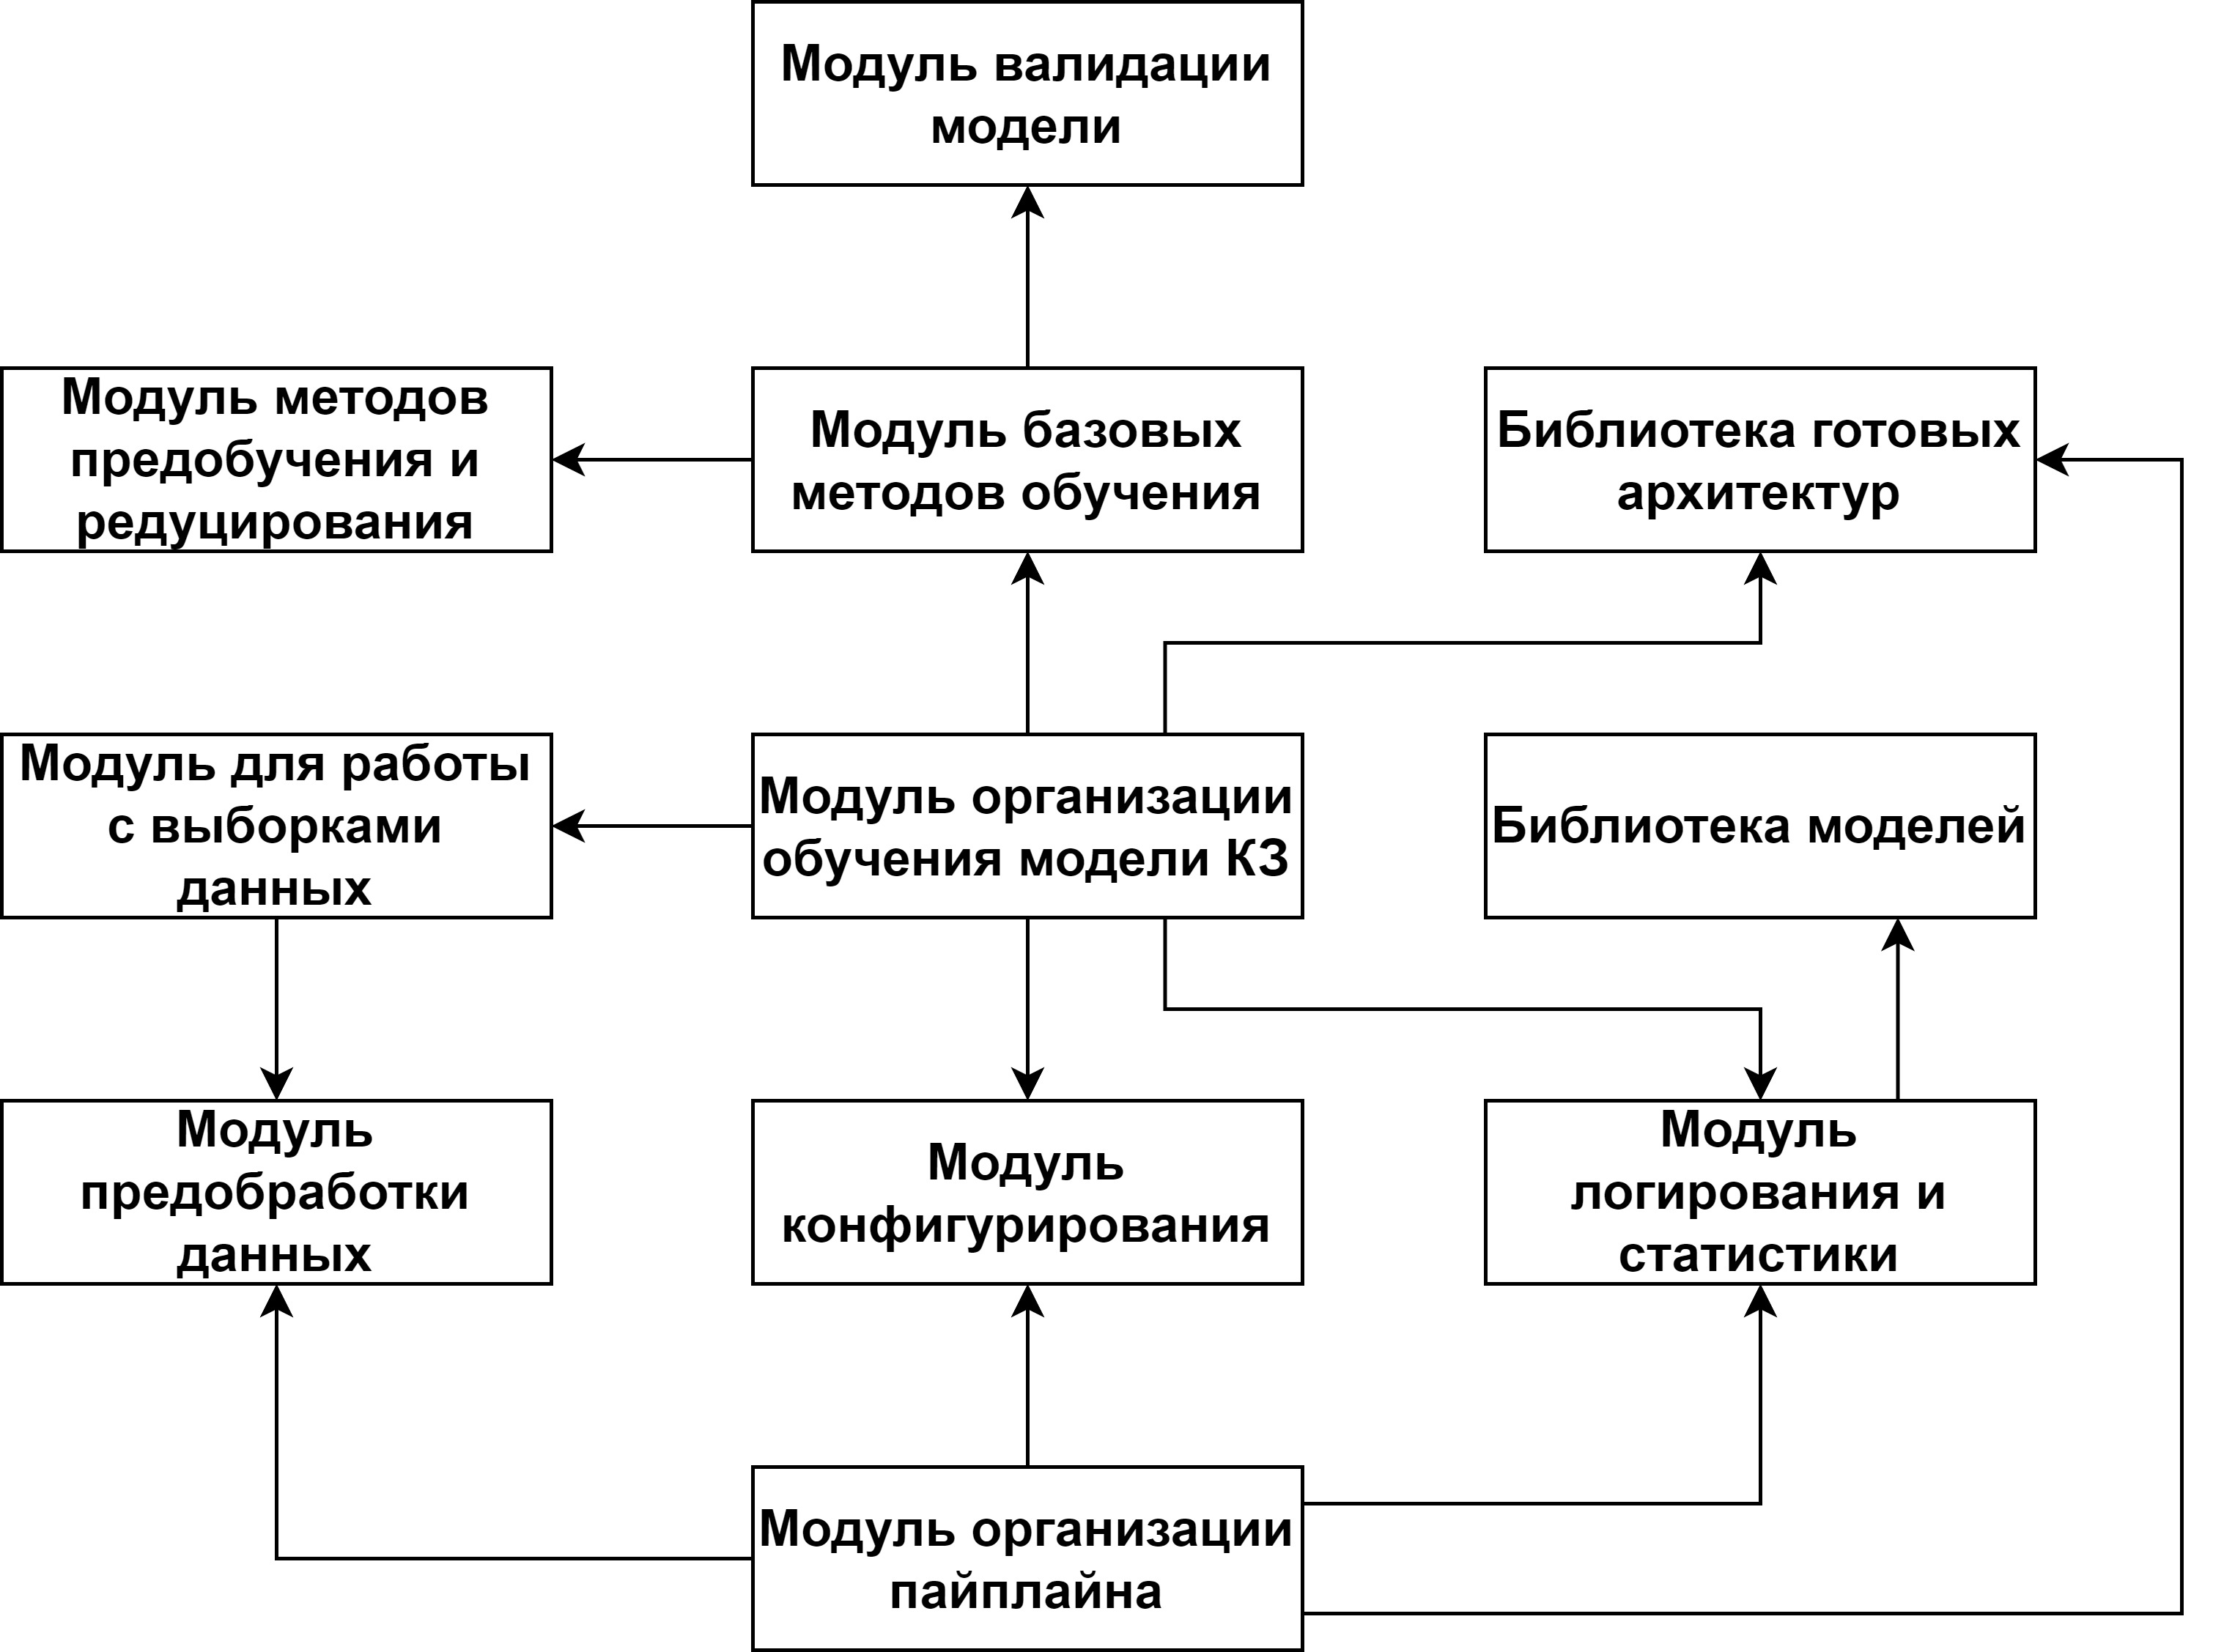
\includegraphics[width=0.8\textwidth]{pic4-0.jpg}
            \end{figure}
        \end{frame}

        \begin{frame}{Cистема обнаружения солнечных панелей на аэрофотоснимках}
            \small
            \begin{block}{Цель разработки}
                Разработать систему детекции солнечных панелей на фотоснимках, полученных из выборки, собранной из Google Maps
            \end{block}
            \begin{block}{Актуальность}
                Необходимость разработки специализированных решений для детекции панелей обусловлена стремлением компаний получать информацию об применении данной технологии и тем самым создавать целевое предложение.
            \end{block}
            
            \begin{columns}
                \begin{column}{0.5\textwidth}
                    Предлагаемый алгоритм обнаружения панелей включает два основных этапа, на каждом из которых используется предобученная глубокая нейронная сеть: 

                    \begin{enumerate}
                    \item Оценка наличия солнечной панели на аэрофотоснимке
                    \item Локализация солнечной панели
                    \end{enumerate}
                \end{column}
                \begin{column}{0.5\textwidth}
                    \begin{figure}
                        \centering
                        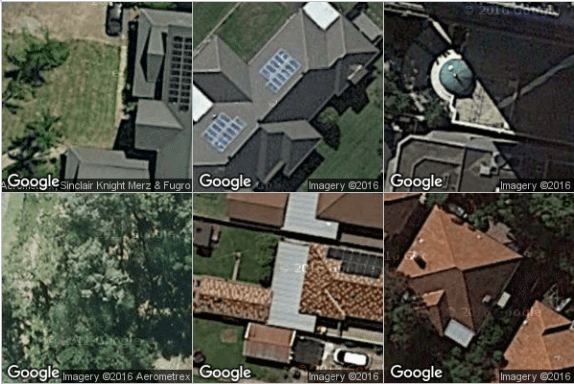
\includegraphics[width=0.9\textwidth]{pic4-17.png}
                    \end{figure}
                \end{column}
            \end{columns}
        \end{frame}

        \begin{frame}{Схема алгоритма для обнаружения солнечных панелей}
            \begin{figure}
                \centering
                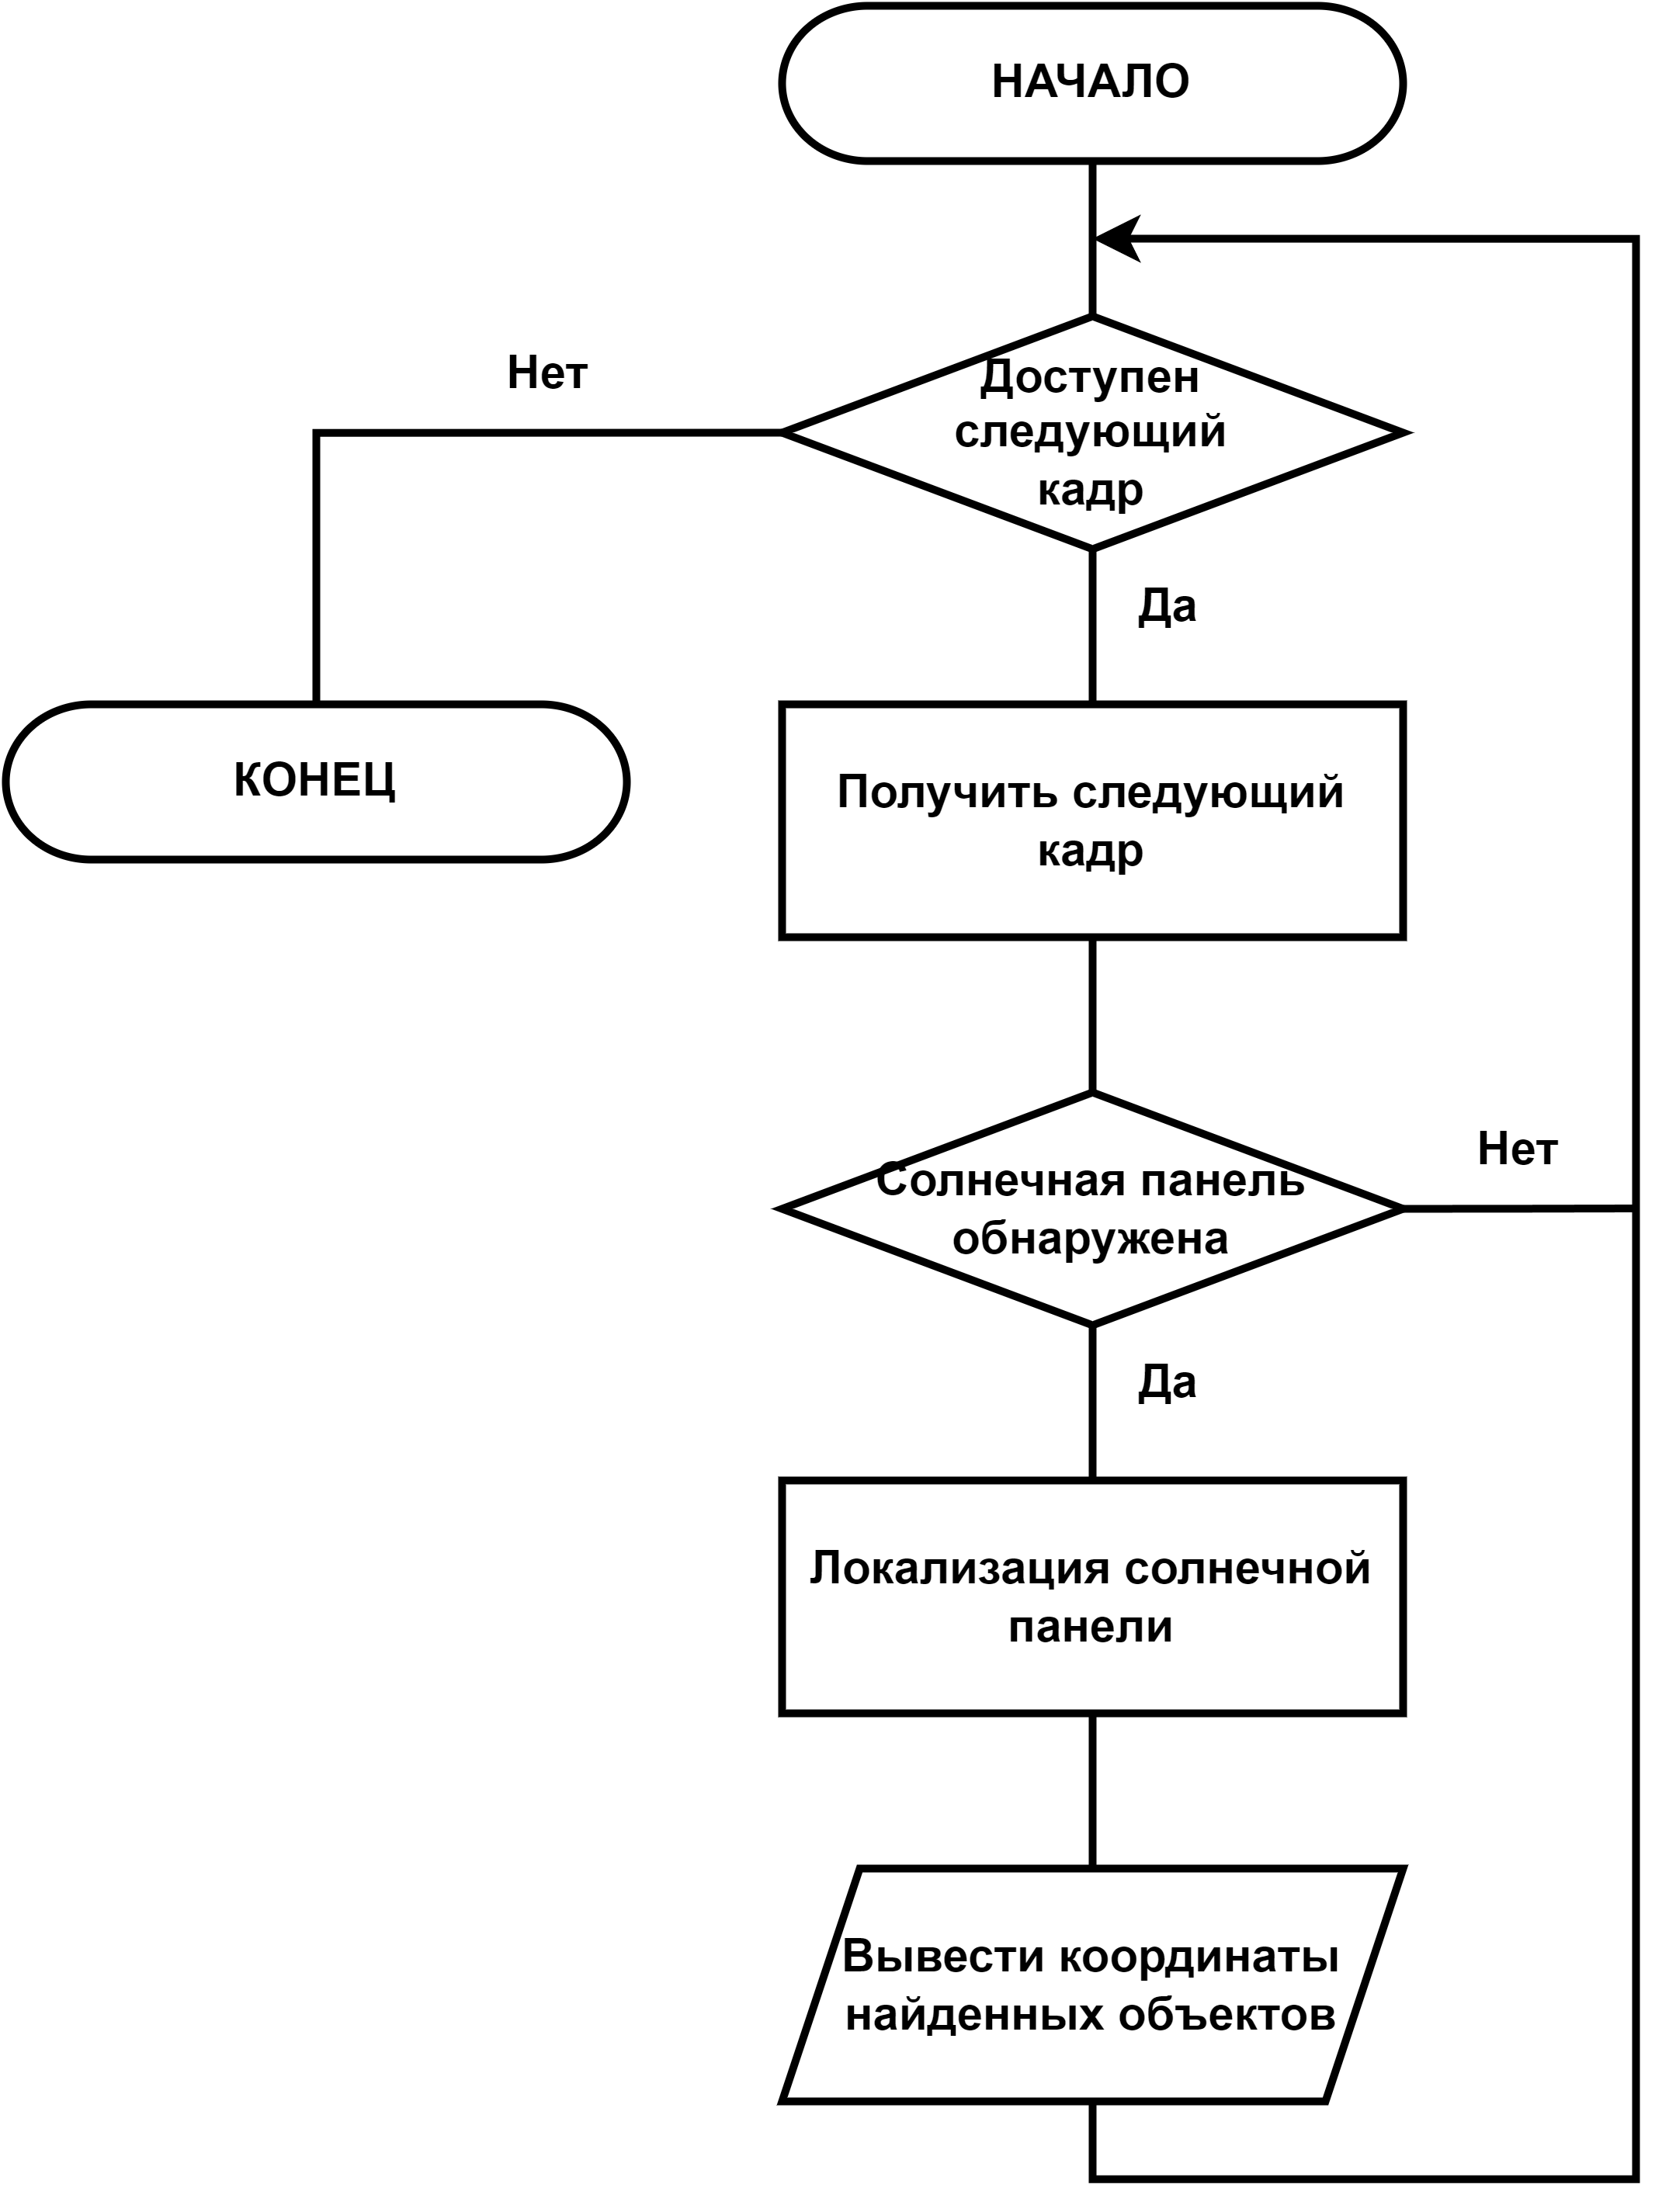
\includegraphics[width=0.5\textwidth]{pic4-16a.png}
            \end{figure}
        \end{frame}

        \begin{frame}{Применяемые модели}
            \underline{Классификатор для оценки наличия панели}
            \begin{figure}
                \centering
                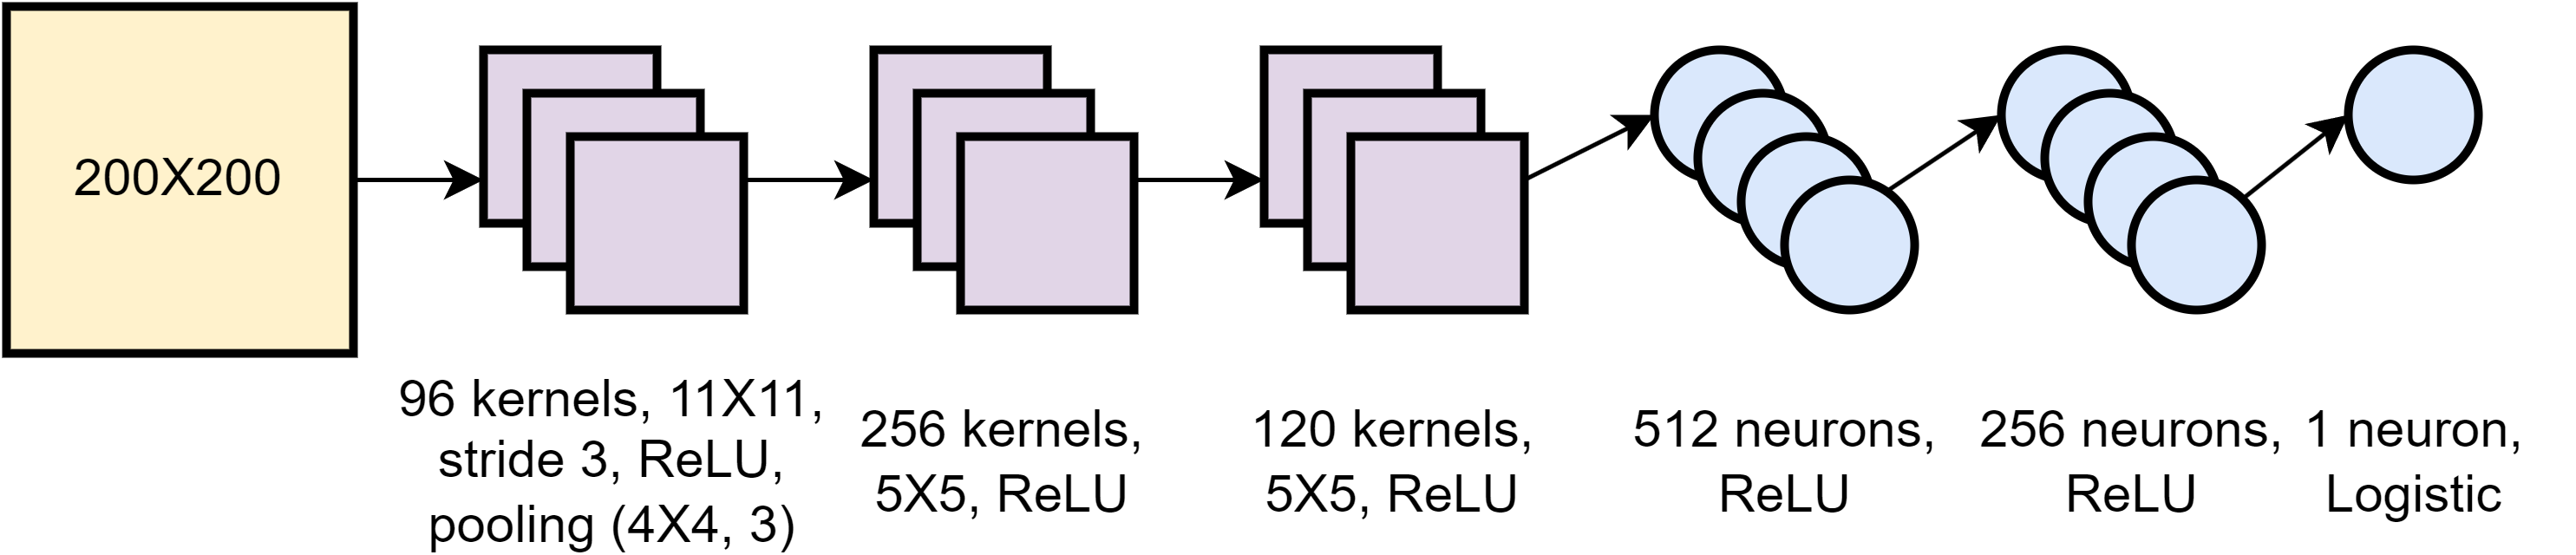
\includegraphics[width=1\textwidth]{pic4-19.png}
            \end{figure}
            \underline{Модель для детекции панели (на базе Faster R-CNN)}
            \begin{figure}
                \centering
                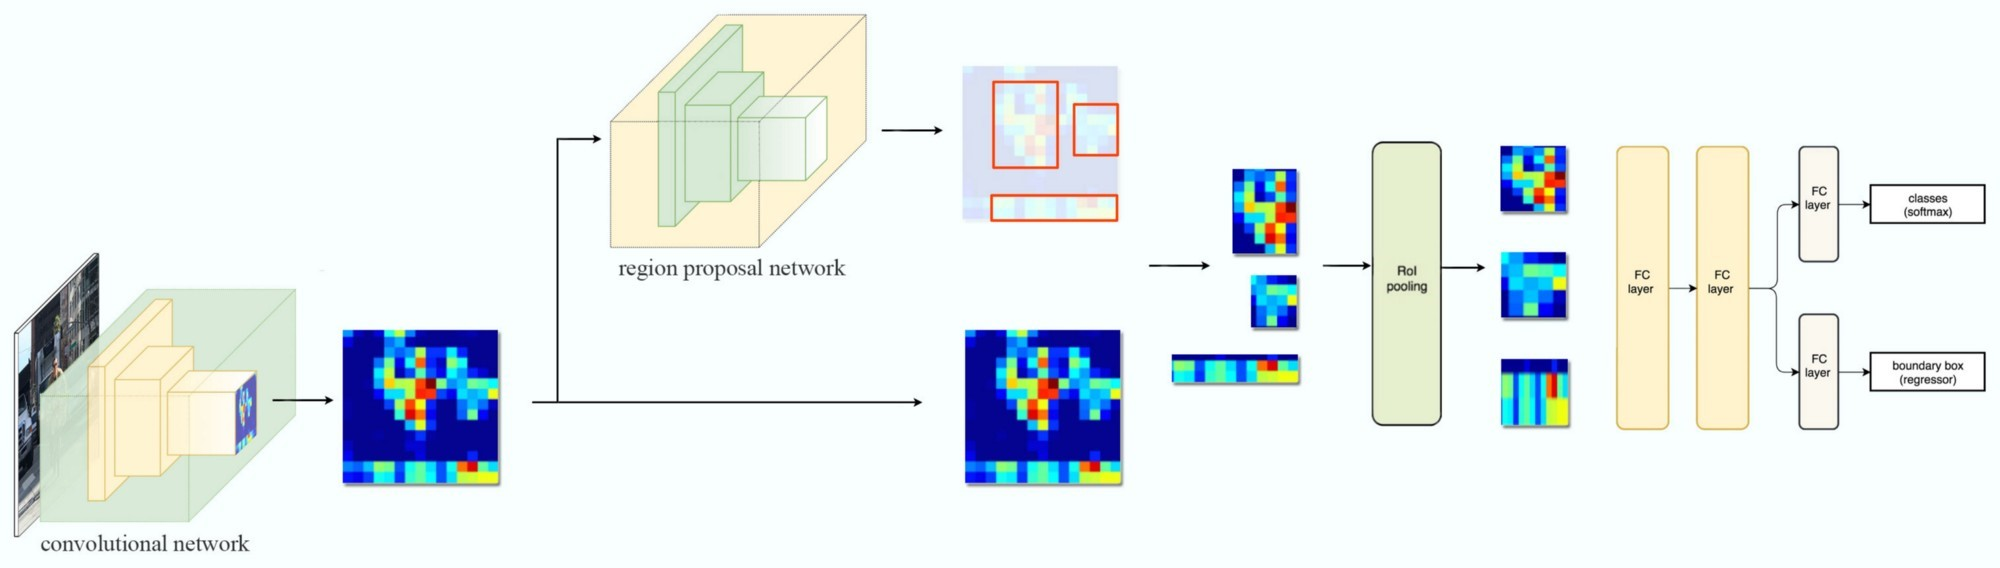
\includegraphics[width=1\textwidth]{pic4-21.jpg}
            \end{figure}
        \end{frame}

        \begin{frame}{Результаты обучения и тестирования моделей (1)}
            \begin{columns}
                \begin{column}{0.55\textwidth}
                \begin{table}
                    \centering
                    \begin{tabular}{| p{2.3cm} | p{2.3cm} | p{1cm} | }
                        \hline
                        \textbf{Модель} & 
                        \textbf{Выборка} & \textbf{Тест., \%}\\
                        \hline
                        Классификатор наличия & Обучающая часть: 2.677\newline
                        Валидационная часть: 
                        670 & 87,46\\
                        \hline
                        Детектор солнечной панели & Обучающая часть:
                        800\newline
                        Валидационная часть:
                        200 & 92,99\\
                        \hline
                    \end{tabular}
                \end{table} 
                \end{column}
                \begin{column}{0.45\textwidth}
                    \begin{figure}
                        \centering
                        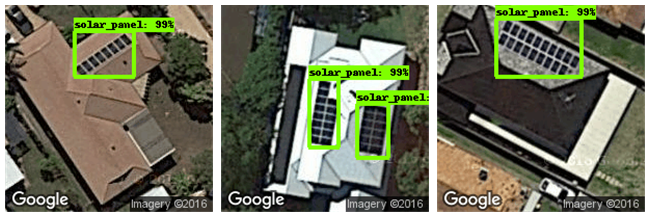
\includegraphics[width=0.9\textwidth]{pic4-22.png}
                    \end{figure}
                    \begin{figure}
                        \centering
                        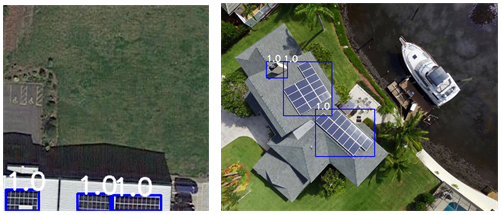
\includegraphics[width=0.9\textwidth]{pic4-23.png}
                    \end{figure}
                \end{column}
            \end{columns}
        \end{frame}

        \begin{frame}{Система распознавания маркировки}
            \small
            \begin{block}{Цель разработки}
                Разработать систему проверки корректности нанесения маркировки на продукцию, производимую ОАО <<Савушкин продукт>>
            \end{block}

            \begin{block}{Актуальность}
                Контроль качества маркировки необходим для контроля за свежестью продукции как со стороны покупателей, так и со стороны обслуживающего персонала супермаркетов, поскольку в большинстве случаев визуальная оценка оказывается проще и быстрее применения специализированных технических средств.
            \end{block}
            
            \begin{columns}
                \begin{column}{0.4\textwidth}
                    \begin{figure}[H]
                        \centering
                        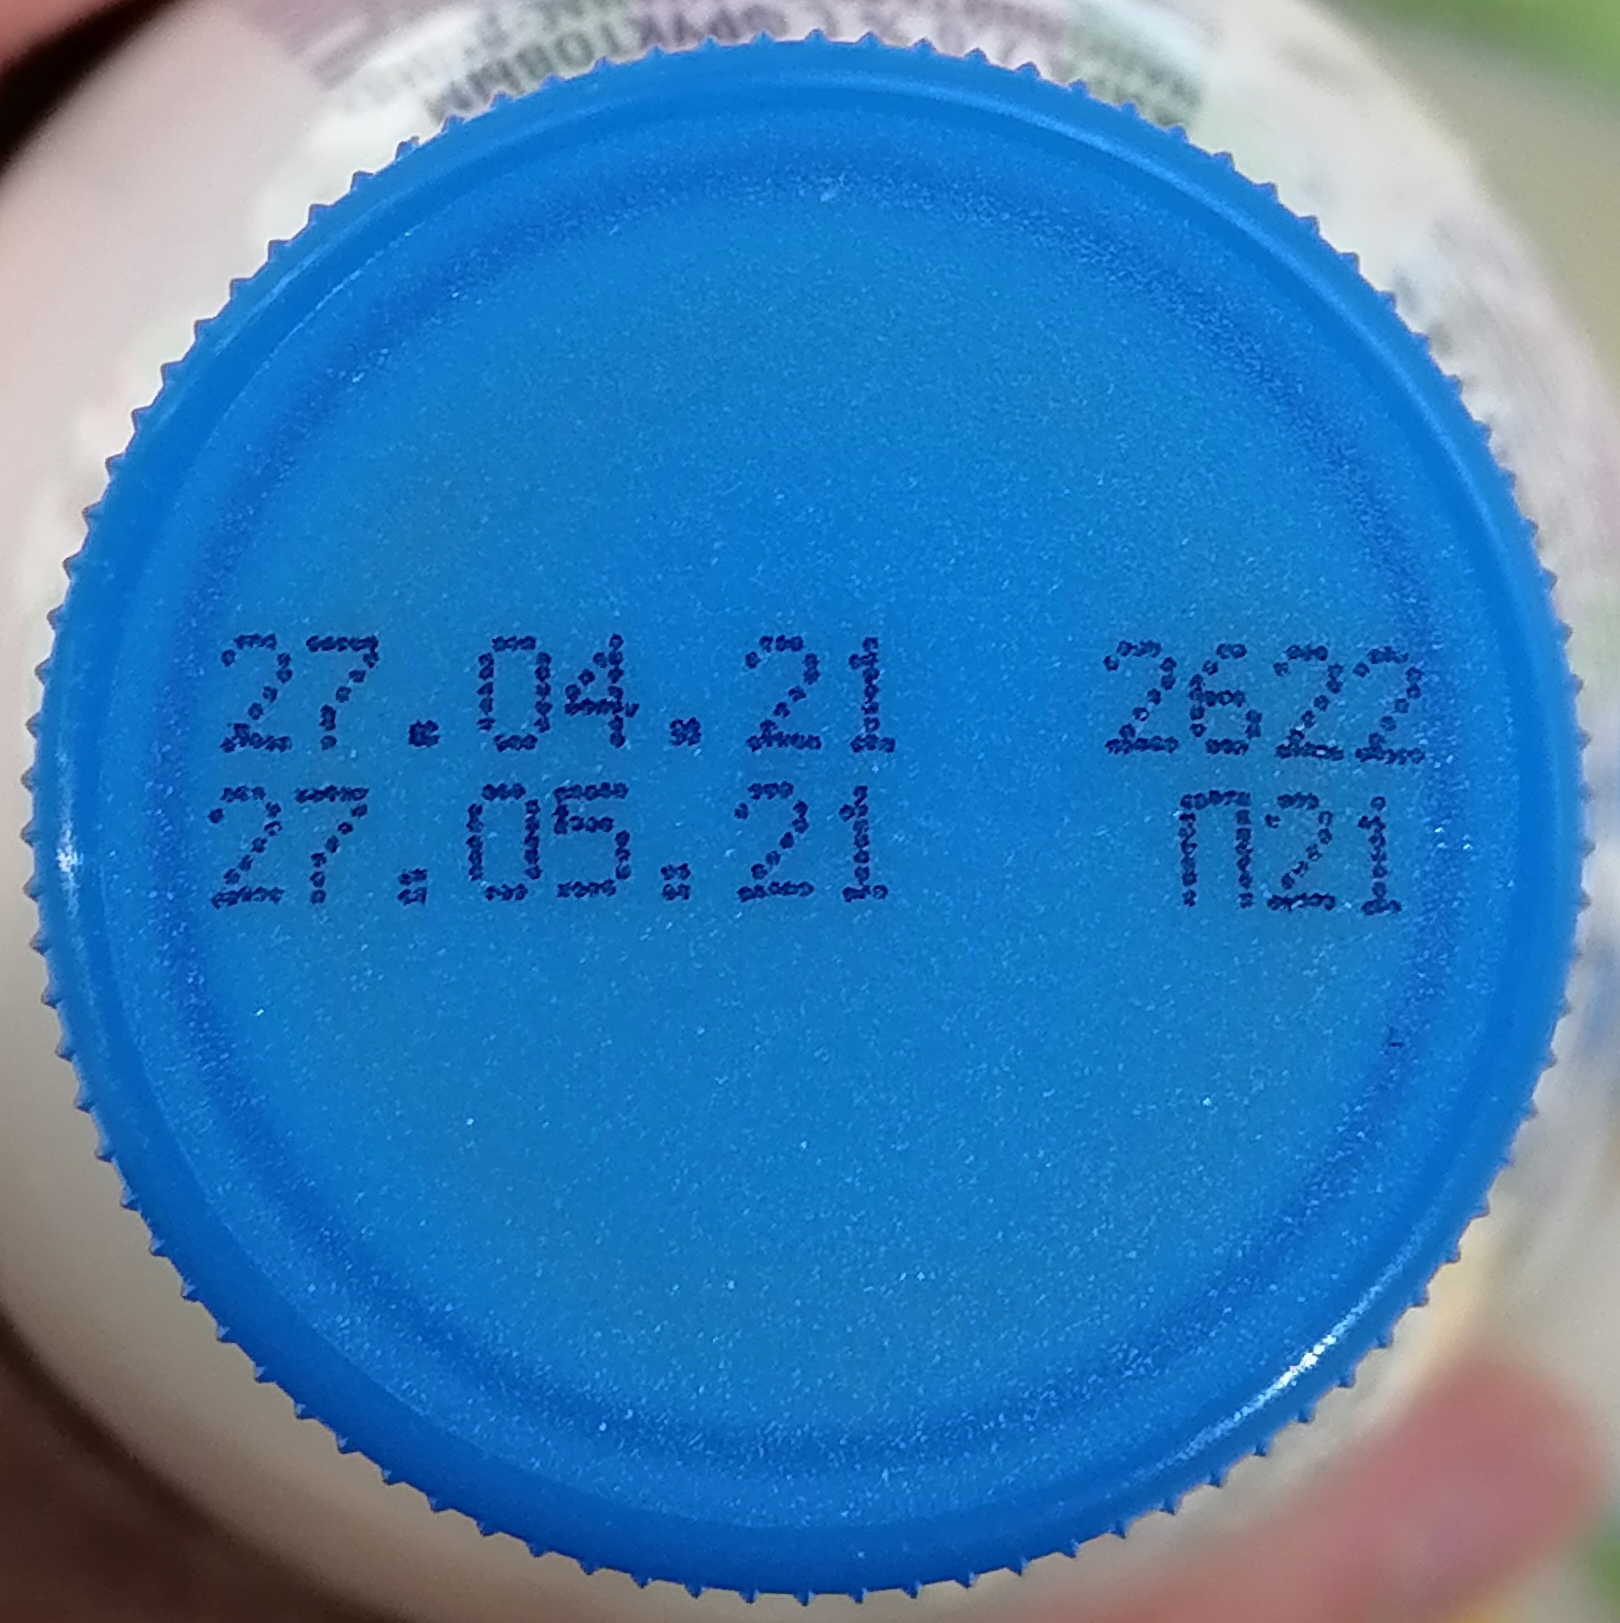
\includegraphics[width=0.7\textwidth]{pic4-1.jpg}
                    \end{figure}
                \end{column}
                \begin{column}{0.4\textwidth}
                    \begin{figure}[H]
                        \centering
                        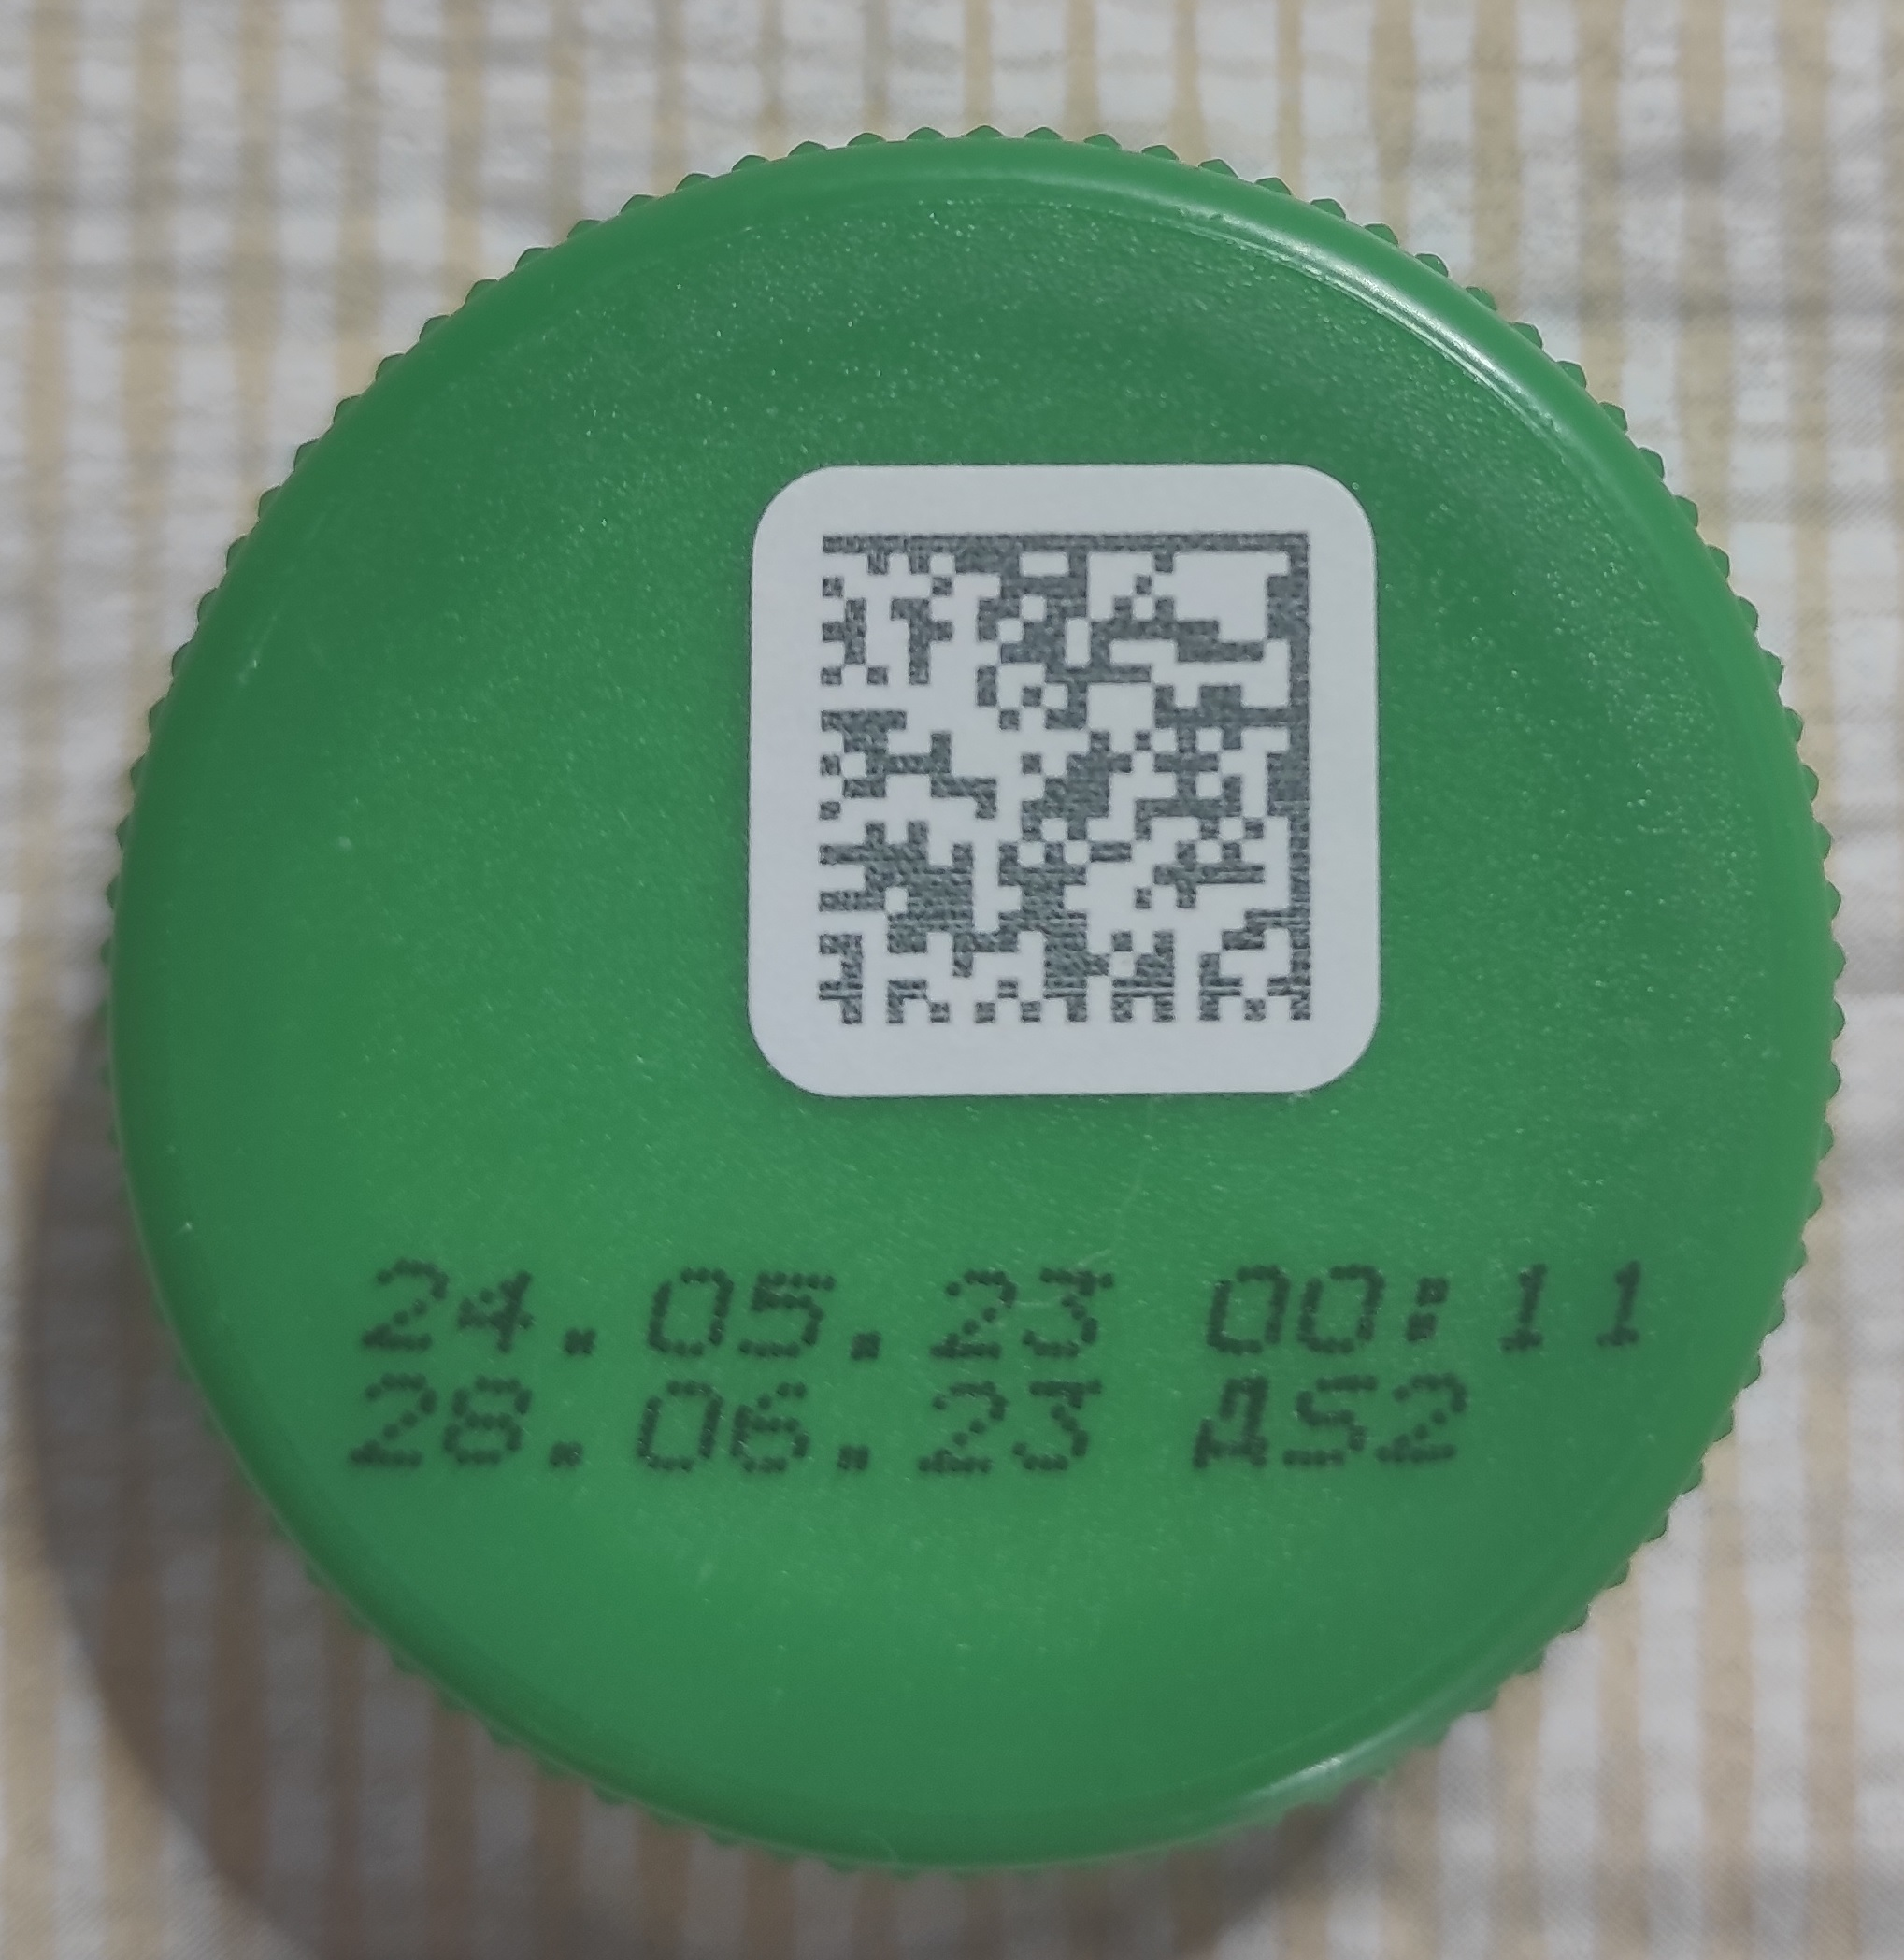
\includegraphics[width=0.7\textwidth]{cap_new.jpg}
                    \end{figure}
                \end{column}
            \end{columns}
        \end{frame}

        \begin{frame}{Возможные ошибки, допускаемые при нанесении маркировки}
            \begin{itemize}
                \item Отсутствие краски в печатающем устройстве;
                \item Смазанность маркировки;
                \item Ошибочная дата в маркировке.
            \end{itemize}

            Первый тип ошибок может быть представлен различными случаями, такими как полное отсутствие маркировки или отсутствие какой-либо ее части.
        \end{frame}

        \begin{frame}{Структура системы и базовые модули}
            \begin{figure}[H]
                \centering
                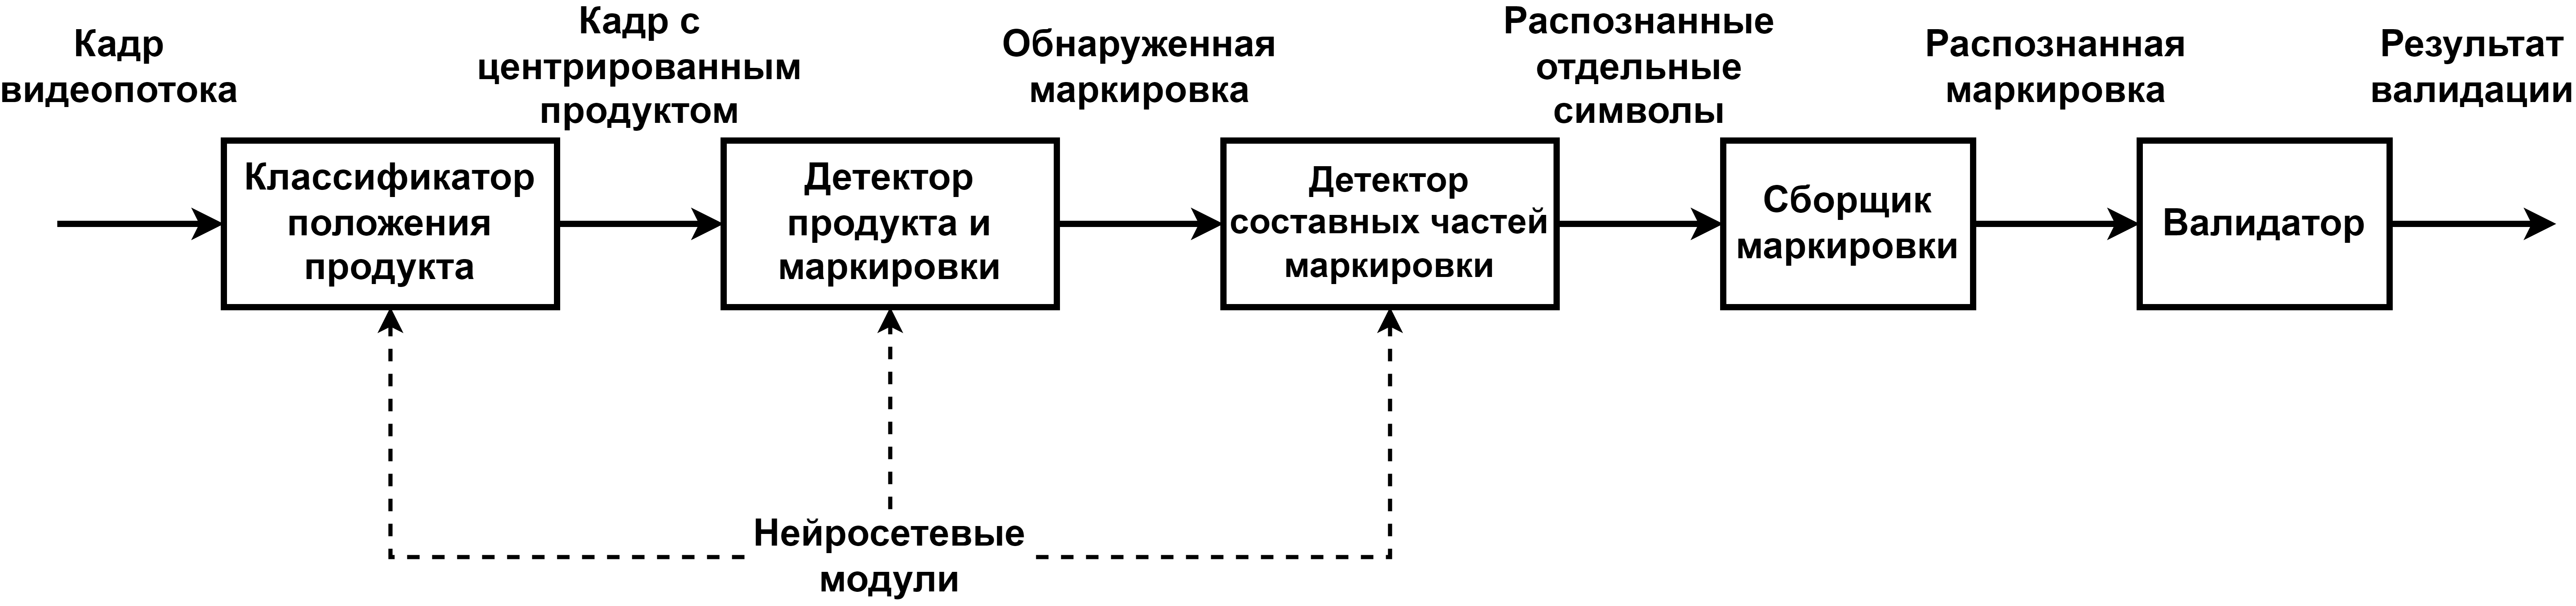
\includegraphics[width=\textwidth]{savushkin_structure.png}
            \end{figure}
            \begin{columns}
                \begin{column}{0.4\textwidth}
                    \begin{enumerate}
                        \item Классификатор положения продукта
                        \item Детектор продукта и маркировки (SSD-MobileNet)
                        \item Детектор составных частей маркировки (SSD-MobileNet)
                    \end{enumerate}
                \end{column}
                \begin{column}{0.6\textwidth}
                    \begin{figure}
                        \centering
                        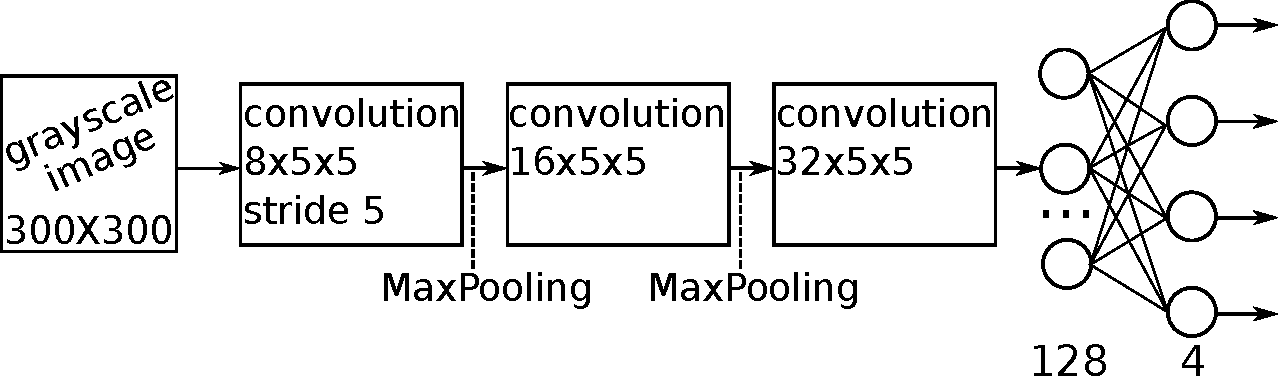
\includegraphics[width=\textwidth]{pic4-4.pdf}
                    \end{figure}
                    \begin{figure}
                        \centering
                        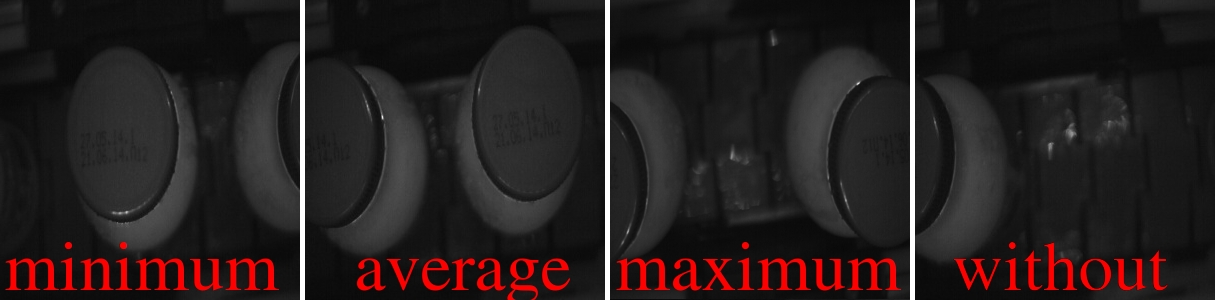
\includegraphics[width=\textwidth]{pic4-24.jpeg}
                    \end{figure}
                \end{column}
            \end{columns}
        \end{frame}

        \begin{frame}{Результаты обучения и тестирования моделей (2)}
            % Используемые выборки и режимы обучения
            \begin{columns}
                \begin{column}{0.55\textwidth}
                    \begin{table}
                        \centering
                        \begin{tabular}{| p{2.3cm} | p{2.3cm} | p{1cm} | }
                          \hline
                            \textbf{Модель} & 
                            \textbf{Выборка} & \textbf{Тест., \%}\\
                            \hline
                            Классификатор положения продукта & Обучающая часть: 4.886\newline
                            Валидационная часть: 
                            1.303 & 93,27\\
                            \hline
                            Детектор продукта и маркировки & Обучающая часть:
                            652\newline
                            Валидационная часть:
                            163 & 99,03\\
                            \hline
                            Детектор отдельных символов & Обучающая часть:
                            33402 (SVHN) + 825\newline
                            Валидационная часть:
                            13068 (SVHN) + 275 & 92,43\\
                            \hline
                        \end{tabular}
                    \end{table}  
                \end{column}
                \begin{column}{0.45\textwidth}
                    \begin{figure}
                        \centering
                        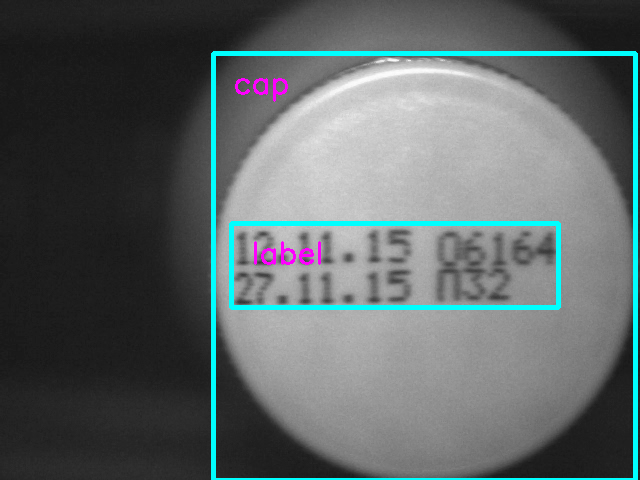
\includegraphics[width=\textwidth]{pic4-25.png}
                    \end{figure}
                    \begin{figure}
                        \centering
                        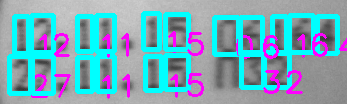
\includegraphics[width=3cm]{pic4-26.png}
                    \end{figure}
                \end{column}
            \end{columns}
        \end{frame}

        \begin{frame}{Связь работы с научными программами}
            \begin{enumerate}
                \item НИР МОРБ <<Алгоритмы интеллектуального анализа и обработки больших объемов данных на основе нейронных сетей глубокого доверия>> (ГБ~15/203, №~госрегистрации~20150743),
                \item ГПНИ <<Информатика и космос, научное обеспечение безопасности и защиты от чрезвычайных ситуаций>> по заданию <<Нейросетевые методы обработки комплексной информации и принятия решений на основе интеллектуальных многоагентных систем>> (№~госрегистрации~20140547),
                \item \small{ГПНИ <<Информатика и космос, научное обеспечение безопасности и защиты от чрезвычайных ситуаций>> по заданию <<Методы и алгоритмы интеллектуальной обработки и анализа большого объема данных на основе нейронных сетей глубокого доверия>> (задание~1.6.05, №~госрегистрации~20163595)},
                \item НИР <<Методы и алгоритмы построения интеллектуальных систем анализа и обработки данных>>, этап <<Разработка гибридных интеллектуальных систем на основе нейросимволического подхода>> (решение НТС УО <<Брестский государственный технический университет>> от 12.11.2021, протокол №~6, №~22202052022070),
                \item НИР БРФФИ <<Модели и исследование 3-D оцифровки на основе фактических данных и анализа гетерогенных данных>> (№~Ф22КИ-046 от 05.11.2021 г., №~госрегистрации 20220090).            
            \end{enumerate}
        \end{frame}

        \begin{frame}[shrink=5]{Апробация результатов диссертации}
            \small
            \underline{Международные конференции:}
            \begin{enumerate}
                \item Открытые семантические технологии проектирования интеллектуальных систем (\textbf{\textit{Минск, 2018-2023}}).
                \item International Conference on Neural Networks and Artificial Intelligence (\textbf{\textit{Брест, 2014}});
                \item Информационное, программное и техническое обеспечение систем управления организационно-технологическими комплексами (\textbf{\textit{Луцк, 2015}});
                \item 8th International Joint Conference on Computational Intelligence (IJCCI) (\textbf{\textit{Порто, 2016}});
                \item 8th, 9th, 11th IEEE International Conference on Intelligent Data Acquisition and Advanced Computing Systems: Technology and Applications (IDAACS) (\textbf{\textit{Варшава, 2015; Бухарест, 2017; Краков, 2021}}); 
                \item International Scientific-Practical Conference Problems of Infocommunications. Science and Technology (PIC S\&T) (\textbf{\textit{Харьков, 2018}});
                \item International Conference on Pattern Recognition and Information Processing (PRIP) (\textbf{\textit{Минск, 2019}});
            \end{enumerate}
            \underline{Республиканские конференции:}
            \begin{itemize}
                \item Вычислительные методы, модели и образовательные технологии \\ (\textbf{\textit{Брест, 2013-2016, 2019}})
                \item Современные проблемы математики и вычислительной техники \\ (\textbf{\textit{Брест, 2015, 2019, 2021}})
            \end{itemize}
        \end{frame}

        \begin{frame}{Опубликованность результатов диссертации (1)}
            Основные результаты диссертационного исследования опубликованы в~30 научных работах, среди которых: 
            \begin{itemize}
                \item 8 статей в научных изданиях в соответствии с пунктом 19 Положения о присуждении ученых степеней и присвоении ученых званий (общим объемом 3,87 авторского листа);
                \item 5 статей в других научных изданиях;
                \item 13 статей в сборниках материалов научных конференций;
                \item 4 тезисов.
            \end{itemize}
        \end{frame}

        \begin{frame}{Опубликованность результатов диссертации (2)}
            \footnotesize
            \justifying
            \textbf{Статьи в научных рецензируемых изданиях, включенных в перечень изданий, и в иностранных научных изданиях}
            \begin{enumerate}
                \item \justifying{Головко, В.А. Персептроны и нейронные сети глубокого доверия : обучение и применение / В.А. Головко, А.А. Крощенко // Вестник Брестского государственного технического университета. Физика, математика, информатика. --- 2014. --- №~5 (89). --- С. 2–-12.}
                \item \justifying{Golovko, V. The Nature of Unsupervised Learning in Deep Neural Networks : A New Understanding and Novel Approach / V. Golovko, A. Kroshchanka, D. Treadwell // Optical Memory and Neural Networks. --- 2016. --- Vol. 25, №~3. --- P. 127--141.}
                \item \justifying{Головко, В.А. Теория глубокого обучения : конвенциальный и новый подход / В.А. Головко, А.А. Крощенко, М.В. Хацкевич // Вестник Брестского государственного технического университета. Физика, математика, информатика. --- 2016. --- №~5 (101). --- С. 7--16.}
                \item \justifying{Крощенко, А.А. Реализация нейросетевой системы распознавания маркировки продукции / А.А. Крощенко, В.А. Головко // Вестник Брестского государственного технического университета. Физика, математика, информатика. --- 2019. --- №~5 (118). --- С. 9--12.}
                \item \justifying{Golovko, V.A. Deep Neural Networks : Selected Aspects of Learning and Application / V.A. Golovko, A.A. Kroshchanka, E.V. Mikhno // Pattern Recognition and Image Analysis. --- 2021. --- Vol. 31, №~1. --- P. 132--143.}
                \item \justifying{Kroshchanka, A. Neural network component of the product marking recognition system on the production line / A. Kroshchanka, D. Ivaniuk // Open Semantic Technologies for Intelligent Systems : research papers collection / Belar. State Univ. of Informatics and Radioelectr.; ed. : V.V. Golenkov (ed.-in-chief) [et al.]. --- Minsk, 2021. --- Iss. 5. --- P. 219--224.}
            \end{enumerate}
        \end{frame}

        \begin{frame}{Опубликованность результатов диссертации (3)}
            \footnotesize
            \justifying
            \begin{enumerate}
                \setcounter{enumi}{6}
                \item \justifying{Kroshchanka, A.A. Method for Reducing Neural-Network Models of Computer Vision / A.A. Kroshchanka, V.A. Golovko, M. Chodyka // Pattern Recognition and Image Analysis. --- Berlin, Heidelberg : Springer-Verlag, 2022. --- Vol. 32, №~2. --- P. 294--300.}
                \item \justifying{Kroshchanka, A.A. Reduction of Neural Network Models in Intelligent Computer Systems of a New Generation / A. Kroshchanka // Open Semantic Technologies for Intelligent Systems (OSTIS-2023) : research papers collection / Belar. State Univ. of Informatics and Radioelectr.; ed. : V.V. Golenkov (ed.-in-chief) [et al.]. --- Minsk, 2023. --- Iss. 7. --- P. 127--132.}
            \end{enumerate}
            \textbf{Статьи в других научных изданиях}
            \begin{enumerate}
                \item \justifying{Головко, В.А. Метод обучения нейронной сети глубокого доверия и применение для визуализации данных / В.А. Головко, А.А. Крощенко // Комп’ютерно-iнтегрованi технологiї: освiта, наука, виробництво. --- Луцьк, 2015. --- №~19. --- С. 6--12.}
                \item \justifying{Интеграция искусственных нейронных сетей с базами знаний / В.А. Головко, В.В. Голенков, В.П. Ивашенко, В.В. Таберко, Д.С. Иванюк, А.А. Крощенко, М.В. Ковалёв // Онтология проектирования. --- 2018. --- Т. 8. --- №~3 (29). --- С. 366--386.}
                \item \justifying{Principles of decision-making systems building based on the integration of neural networks and semantic models / V. Golovko, A. Kroshchanka, V. Ivashenko, M. Kovalev, V. Taberko, D. Ivaniuk // Open Semantic Technologies for Intelligent Systems (OSTIS-2019) : research papers collection / Belar. State Univ. of Informatics and Radioelectr.; ed. : V.V. Golenkov (ed.-in-chief) [et al.]. --- Minsk, 2019. --- Iss. 3. --- P. 91--102.}
            \end{enumerate}
        \end{frame}

        \begin{frame}{Опубликованность результатов диссертации (4)}
            \footnotesize
            \justifying
            \begin{enumerate}
                \setcounter{enumi}{3}
                \item \justifying{Implementation of an intelligent decision support system to accompany the manufacturing process / V. Golovko, A. Kroshchanka, M. Kovalev, V. Taberko, D. Ivaniuk // Open Semantic Technologies for Intelligent Systems (OSTIS-2020) : research papers collection / Belar. State Univ. of Informatics and Radioelectr.; ed. : V.V. Golenkov (ed.-in-chief) [et al.]. --- Minsk, 2020. --- Iss. 4. --- P. 175--182.}
                \item \justifying{Deep Convolutional Neural Network for Detection of Solar Panels / V. Golovko, A. Kroshchanka, E. Mikhno, M. Komar, A. Sachenko // Data-Centric Business and Applications. ICT Systems-Theory, Radio-Electronics, Information Technologies and Cybersecurity. --- Cham: Springer International Publishing, 2021. --- P. 371--389.}
            \end{enumerate}
            \textbf{Статьи в сборниках материалов научных конференций}
            \begin{enumerate}
                \item \justifying{A Learning Technique for Deep Belief Neural Networks / V. Golovko, A. Kroshchanka, U. Rubanau, S. Jankowski // Neural Networks and Artificial Intelligence : proc. of the 8th Internat. Conf. ICNNAI 2014, Brest, Belarus, June 3-6, 2014 / V. Golovko, A. Imada (eds.). --- Springer, 2014. --- P. 136--146.}
                \item \justifying{Головко, В.А. Применение нейронных сетей глубокого доверия для выделения семантически значимых признаков / В.А. Головко, А.А. Крощенко // Открытые семантические технологии проектирования интеллектуальных систем : материалы V Междунар. науч.-технич. конф. OSTIS-2015, Минск, 19-21 февраля 2015 г. / УО <<Бел. гос. ун-т информатики и радиоэлектроники>>, ГУ <<Администрация Парка высоких технологий>>; редкол.: В.В. Голенков (отв. ред.) [и др.]. --- Минск, 2015. --- P. 481--486.}
            \end{enumerate}  
        \end{frame}

        \begin{frame}{Опубликованность результатов диссертации (5)}
            \footnotesize
            \justifying
            \begin{enumerate}
                \setcounter{enumi}{2}
                \item \justifying{A New Technique for Restricted Boltzmann Machine Learning [Electronic resource] / V. Golovko, A. Kroshchanka, V. Turchenko, S. Jankowski, D. Treadwell // Proceedings of the 8th IEEE International Conference of Intelligent Data Acquisition and Advanced Computing Systems : Technology and Applications (IDAACS), Warsaw, Poland, Sept. 24-26, 2015 / Research Institute for Intelligent Computer Systems, Ternopil National Economic University and V.M. Glushkov Inst. of Cybernetics, National Academy for Sciences of Ukraine, Warsaw University of Technology. --- P. 182--186. --- Mode of access : \url{https://ieeexplore.ieee.org/document/7340725}. --- Date of access : 05.06.2023.}
                \item \justifying{Крощенко, А.А. Применение нейронных сетей глубокого доверия в \\ интеллектуальном анализе данных / А.А. Крощенко // Современные проблемы математики и вычислительной техники : сб. материалов IX Респ. науч. конф. молодых ученых и студентов, Брест, 19-21 ноября 2015 г. / Мин. обр. Респ. Бел., УО <<Брест. гос. технич. ун-т>>; редкол.: В.С. Рубанов (гл. ред.) [и др.]. --- Брест, 2015. --- С. 12--14.}
                \item \justifying{Golovko, V. Theoretical Notes on Unsupervised Learning in Deep Neural Networks [Electronic resource] / V. Golovko, A. Kroshchanka // Proceedings of the 8th Internat. Joint Conf. on Computational Intelligence (IJCCI 2016), Porto, Portugal, Nov. 9-11 2016. --- P. 91--96. --- Mode of access : \url{https://scitepress.org/papers/2016/60843/60843.pdf}. --- Date of access : 05.06.2023.}
            \end{enumerate}
        \end{frame}

        \begin{frame}{Опубликованность результатов диссертации (6)}
            \footnotesize
            \justifying
            \begin{enumerate}
                \setcounter{enumi}{5}
                \item \justifying{Convolutional Neural Network Based Solar Photovoltaic Panel Detection in Satellite Photos [Electronic resource] / V. Golovko, S. Bezobrazov, A. Kroshchanka, A. Sachenko, M. Komar, A. Karachka // The 9th IEEE Internat. Conf. on Intelligent Data Acquisition and Advanced Computing Systems: Technology and Applications, Bucharest, Romania, Sept. 21-23 2017. --- P. 14--19. --- Mode of access : \url{https://ieeexplore.ieee.org/document/8094501}. --- Date of access : 05.06.2023.}
                \item \justifying{Integration of artificial neural networks and knowledge bases / V.A. Golovko, A.A. Kroshchanka, V.V. Golenkov, V.P. Ivashenko, M.V. Kovalev, V.V. Taberko, D.S. Ivaniuk // Открытые семантические технологии проектирования интеллектуальных систем : материалы VIII Междунар. науч.-технич. конф., Минск, 15-17 февраля 2018 г. / Мин. обр. Респ. Бел., УО <<Бел. гос. ун-т информатики и радиоэлектроники>>; редкол.: В.В. Голенков (гл. ред.) [и др.]. --- Минск, 2018. --- Вып. 2. --- C. 133--146.}
                \item \justifying{Головко, В.А. Нейросетевые модели глубокого обучения для решения задач распознавания объектов на изображении / В.А. Головко, А.А. Крощенко // Вычислительные методы, модели и образовательные технологии : сб. материалов VII Междунар. науч.-практич. конф., Брест, 19 октября 2018 г. / Брест. гос. ун-т имени А.С. Пушкина; под общ. ред. А.А. Козинского. --- Брест, 2018. --- С. 3--5.}
            \end{enumerate}            
        \end{frame}

        \begin{frame}{Опубликованность результатов диссертации (7)}
            \footnotesize
            \justifying
            \begin{enumerate}
                \setcounter{enumi}{8}
                \item \justifying{Golovko, V. Development of Solar Panels Detector [Electronic resource] / V. Golovko, A. Kroshchanka, S. Bezobrazov, A. Sachenko, M. Komar, O. Novosad // 2018 International Scientific-Practical Conference <<Problems of Infocommunications. Science and Technology (PIC S\&T 2018)>>, Kharkiv, Ukraine, 9-12 October 2018 / Institute of Electrical and Electronics Engineers, Inc. --- Mode of access : \url{https://www.semanticscholar.org/paper/Development-of-Solar-Panels-Detector-Golovko-Kroshchanka/914c0b8c159c64100609fc8455636b1e3f8568cb}. --- Date of access : 05.06.2023.}
                \item \justifying{Golovko, V. Brands and caps labeling recognition in images using deep learning [Electronic resource] / V. Golovko, A. Kroshchanka, E. Mikhno // Pattern Recognition and Information Processing : revised selected papers of the 14th Internat. Conf. PRIP 2019, Minsk, May 21-23 2019; Eds. : S.V. Ablameyko, V.V. Krasnoproshin, M.M. Lukashevich. --- P. 35--51. --- Mode of access : \url{https://www.researchgate.net/publication/337459978_Brands_and_Caps_Labeling_Recognition_in_Images_Using_Deep_Learning}. --- Date of access : 05.06.2023.}
                \item \justifying{Головко, В.А. Обнаружение и распознавание маркировки продукции с помощью нейросетевых алгоритмов / В.А. Головко, А.А. Крощенко // Вычислительные методы, модели и образовательные технологии: сб. материалов VII Междунар. науч.-практич. конф., Брест, 18 октября 2019 г. / Брест. гос. ун-т имени А.С. Пушкина; под общ. ред. А.А. Козинского. --- Брест, 2019. --- С. 3--6.}
            \end{enumerate}
        \end{frame}

        \begin{frame}{Опубликованность результатов диссертации (8)}
            \footnotesize
            \justifying
            \begin{enumerate}
                \setcounter{enumi}{11}
                \item \justifying{Neuro-Symbolic Artificial Intelligence: Application for Control the Quality of Product Labeling [Electronic resource] / V. Golovko, A. Kroshchanka, M. Kovalev, V. Taberko, D. Ivaniuk // Open Semantic Technologies for Intelligent Systems : revised selected papers of the 10th Intern. Conf. (OSTIS 2020), Minsk, Febr. 19-22, 2020; / Eds. : V. Golenkov, V. Krasnoproshin, V. Golovko, E. Azarov. --- P. 81--101. --- Mode of access : \url{https://libeldoc.bsuir.by/bitstream/123456789/42395/1/Golovko_Neuro_Symbolic.pdf}. --- Date of access : 05.06.2023.}
                \item \justifying{Kroshchanka, A. The Reduction of Fully Connected Neural Network Parameters Using the Pre-training Technique / A. Kroshchanka, V. Golovko // Proceedings of the 11th IEEE Intern. Conf. on Intelligent Data Acquisition and Advanced Computing Systems : Technology and Applications (IDAACS), Cracow, Poland, September 22-25, 2021 / Cracow University of Technology [et al.]. --- Vol. 2. --- P. 937--941. --- Mode of access : \url{https://www.researchgate.net/publication/357613109_The_Reduction_of_Fully_Connected_Neural_Network_Parameters_Using_the_Pre-training_Technique}. --- Date of access : 05.06.2023.}
            \end{enumerate}
            \textbf{Тезисы}
            \begin{enumerate}
                \item \justifying{Крощенко, А.А. Методы глубокого обучения нейронных сетей / А.А. Крощенко // Вычислительные методы, модели и образовательные технологии : сб. матер. региональной науч.-практич. конф., Брест, 22-23 окт. 2013 г. / Брест. гос. ун-т им. А.С. Пушкина; под общ. ред. О.В. Матысика. — Брест, 2013. — С. 21–22.}
                \item Головко, В.А. Об одном методе обучения нейронных сетей глубокого доверия / В.А. Головко, А.А. Крощенко // Вычислительные методы, модели и образовательные технологии : сб. матер. Междунар. науч.-практич. конф., Брест, 15-16 окт. 2014 г. / Брест. гос. ун-т им. А.С. Пушкина; под общ. ред. О.В. Матысика. --- Брест, 2014. --- С. 98--99.
            \end{enumerate}
        \end{frame}

        \begin{frame}{Опубликованность результатов диссертации (9)}
            \footnotesize
            \begin{enumerate}
                \setcounter{enumi}{2}
                \item \justifying{Головко, В.А. Применение нейронных сетей глубокого доверия в интеллектуальном анализе данных / В.А. Головко, А.А. Крощенко // Вычислительные методы, модели и образовательные технологии : сб. матер. Междунар. науч.-практич. конф., Брест, 22 окт. 2015 г. / Брест. гос. ун-т им. А.С. Пушкина; под общ. ред. О.В. Матысика. — Брест, 2015. — С. 97–98.}
                \item Крощенко, А.А. Применение глубокой нейронной сети для решения задачи распознавания образов / А.А. Крощенко // Вычислительные методы, модели и образовательные технологии : сб. матер. Междунар. науч.-практич. конф., Брест, 21 окт. 2016 г. / Брест. гос. ун-т им. А.С. Пушкина; под общ. ред. О.В. Матысика. --- Брест, 2016. --- С. 132--133.
            \end{enumerate}
        \end{frame}

        % \begin{frame}{Опубликованность результатов диссертации (3)}
        %     \small
        %     \justifying
        %     \begin{enumerate}
        %         \setcounter{enumi}{5}
        %         \item \justifying{Головко, В. А. Интеграция искусственных нейронных сетей с базами знаний / В. А. Головко, В. В. Голенков, В. П. Ивашенко, В. В. Таберко, Д. С. Шаток, А. А. Крощенко, М. В. Ковалёв // Онтология проектирования. --- EBSCO Publishing, 2018. --- Т. 8. --- No 3(29). --- С. 366--386.}
        %         \item \justifying{Крощенко, А. А. Реализация нейросетевой системы распознавания маркировки продукции / А. А. Крощенко, В. А. Головко // Вестник БрГТУ. — Брест, 2019. --- No 5. --- С. 9--12.}
        %         \item \justifying{Golovko, V. Brands and caps labeling recognition in images using deep learning / V. Golovko, A. Kroshchanka, E. Mikhno // International Conference on Pattern Recognition and Information Processing. --- Springer, Cham, 2019. --- P. 35--51.}
        %         \item \justifying{Golovko, V. Deep convolutional neural network for detection of solar panels / V. Golovko, A. Kroshchanka, E. Mikhno, M. Komar, A. Sachenko // Data-Centric Business and Applications. — Springer, Cham, 2021. --- P. 371--389.}
        %         \item \justifying{Golovko, V. A. Deep Neural Networks: Selected Aspects of Learning and Application / V. A. Golovko, A. A. Kroshchanka, E. V. Mikhno // Pattern Recognition and Image Analysis. --- Pleiades Publishing, 2021. --- Vol. 31. --- No 1. --- P. 132--143.}
        %     \end{enumerate}
        % \end{frame}

        % \begin{frame}{Опубликованность результатов диссертации (4)}
        %     \small
        %     \justifying
        %     \begin{enumerate}
        %         \setcounter{enumi}{10}
        %         \item \justifying{Kroshchanka, A. A. Method for Reducing Neural-Network Models of Computer Vision / A. A. Kroshchanka, V. A. Golovko, M. Chodyka // Pattern Recognition and Image Analysis. --- Pleiades Publishing, 2022. --- Vol. 32. --- No 2. --- P. 294--300.}
        %     \end{enumerate}
        %     \textbf{Статьи в сборниках материалов научных конференций, включенных в системы международного цитирования (Scopus, Web of Science и IEEE Xplore digital)}
        %     \begin{enumerate}
        %         \setcounter{enumi}{11}
        %         \item \justifying{Golovko, V. A New Technique for Restricted Boltzmann Machine Learning / A. Kroshchanka, V. Turchenko, S. Jankowski, D. Treadwell // Proceedings of the 8th IEEE International Conference IDAACS--2015, Warsaw 24--26 September 2015. --- Warsaw, 2015. --- P. 182--186.}
        %         \item \justifying{Golovko, V. Theoretical Notes on Unsupervised Learning in Deep Neural Networks / V. Golovko, A. Kroshchanka // Proceedings of the 8th International Joint Conference on Computational Intelligence (IJCCI 2016). --- SCITEPRESS, 2016. --- P. 91--96.}
        %         \item \justifying{Golovko, V. Convolutional neural network based solar photovoltaic panel detection in satellite photos / V. Golovko, S. Bezobrazov, A. Kroshchanka, A. Sachenko, M. Komar, A. Karachka // 9th IEEE International Conference on Intelligent Data Acquisition and Advanced Computing Systems: Technology and Applications (IDAACS). --- IEEE, 2017. --- Vol. 1. --- P. 14--19.}
        %     \end{enumerate}
        % \end{frame}

        % \begin{frame}{Опубликованность результатов диссертации (5)}
        %     \begin{enumerate}
        %         \setcounter{enumi}{14}
        %         \item \justifying{Golovko, V. Development of solar panels detector / V. Golovko, A. Kroshchanka, S. Bezobrazov, A. Sachenko, M. Komar, O. Novosad // International Scientific-Practical Conference Problems of Infocommunications. Science and Technology (PIC S\&T). --- IEEE, 2018. --- P. 761--764.}
        %         \item \justifying{Kroshchanka, A. The Reduction of Fully Connected Neural Network Parameters Using the Pre-training Technique / A. Kroshchanka, V. Golovko // 11th IEEE International Conference on Intelligent Data Acquisition and Advanced Computing Systems: Technology and Applications (IDAACS). --- IEEE, 2021. --- Vol. 2. --- P. 937--941.}
        %     \end{enumerate}
        %     \textbf{Статьи в cборниках материалов научных конференций}
        %     \begin{enumerate}
        %         \item \justifying{Kroshchanka, A. Neural network component of the product marking recognition system on the production line / A. Kroshchanka, D. Ivaniuk // Open Semantic Technologies for Intelligent Systems (OSTIS-2021). --- Minsk : BSUIR, 2021. --- P. 219--224.}
        %         \item \justifying{Kroshchanka, A. Reduction of neural network models in intelligent computer systems of a new generation / A. Kroshchanka // Open Semantic Technologies for Intelligent Systems (OSTIS-2023). --- Minsk : BSUIR, 2023. --- P. 127--132.}
        %     \end{enumerate}
        %     \end{frame}

        \begin{frame}{Опубликованность результатов диссертации (10)}
            \begin{figure}
                \centering
                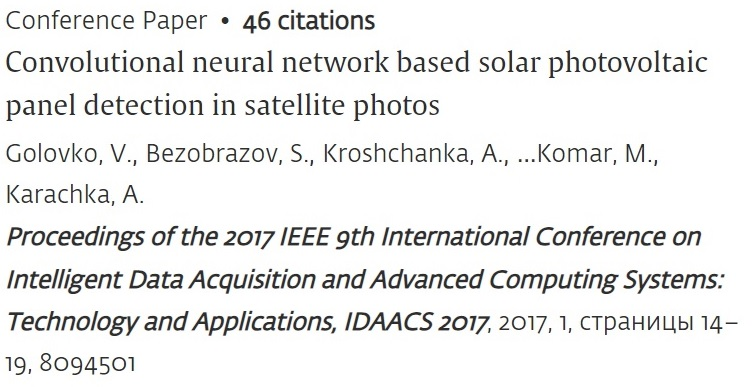
\includegraphics[width=0.5\textwidth]{pub_1.jpg}
            \end{figure}
            \begin{columns}
                \begin{column}{0.45\textwidth}
                    \begin{figure}
                        \centering
                        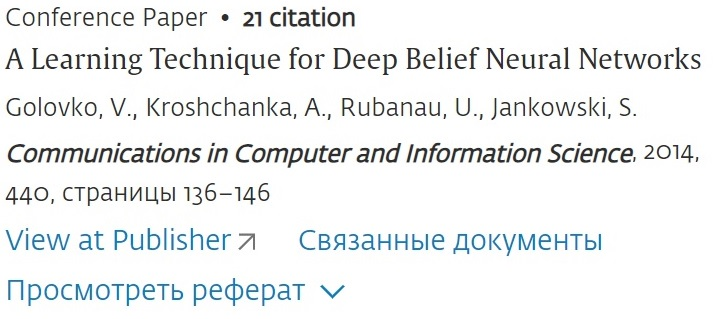
\includegraphics[width=1.1\textwidth]{pub_2.jpg}
                    \end{figure}
                \end{column}
                \begin{column}{0.45\textwidth}
                    \begin{figure}
                        \centering
                        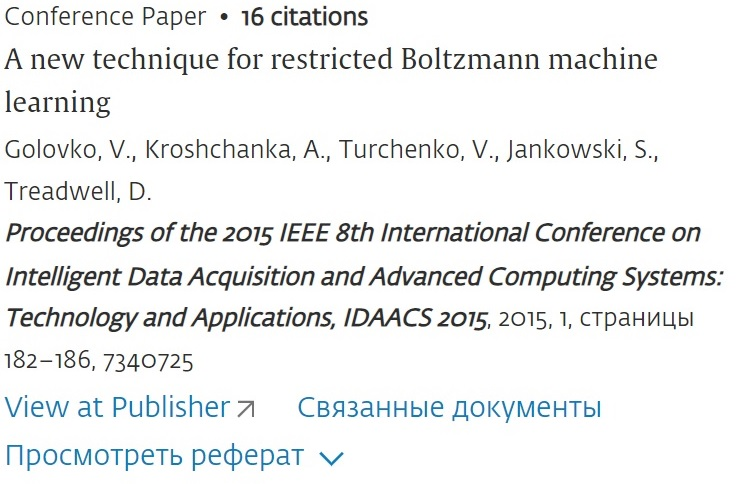
\includegraphics[width=1.1\textwidth]{pub_3.jpg}
                    \end{figure}
                \end{column}
            \end{columns}
        \end{frame}

        \begin{frame}{Внедрение результатов диссертации}
            \begin{figure}
            \centering
            \begin{minipage}[c]{\textwidth}
                \centering
                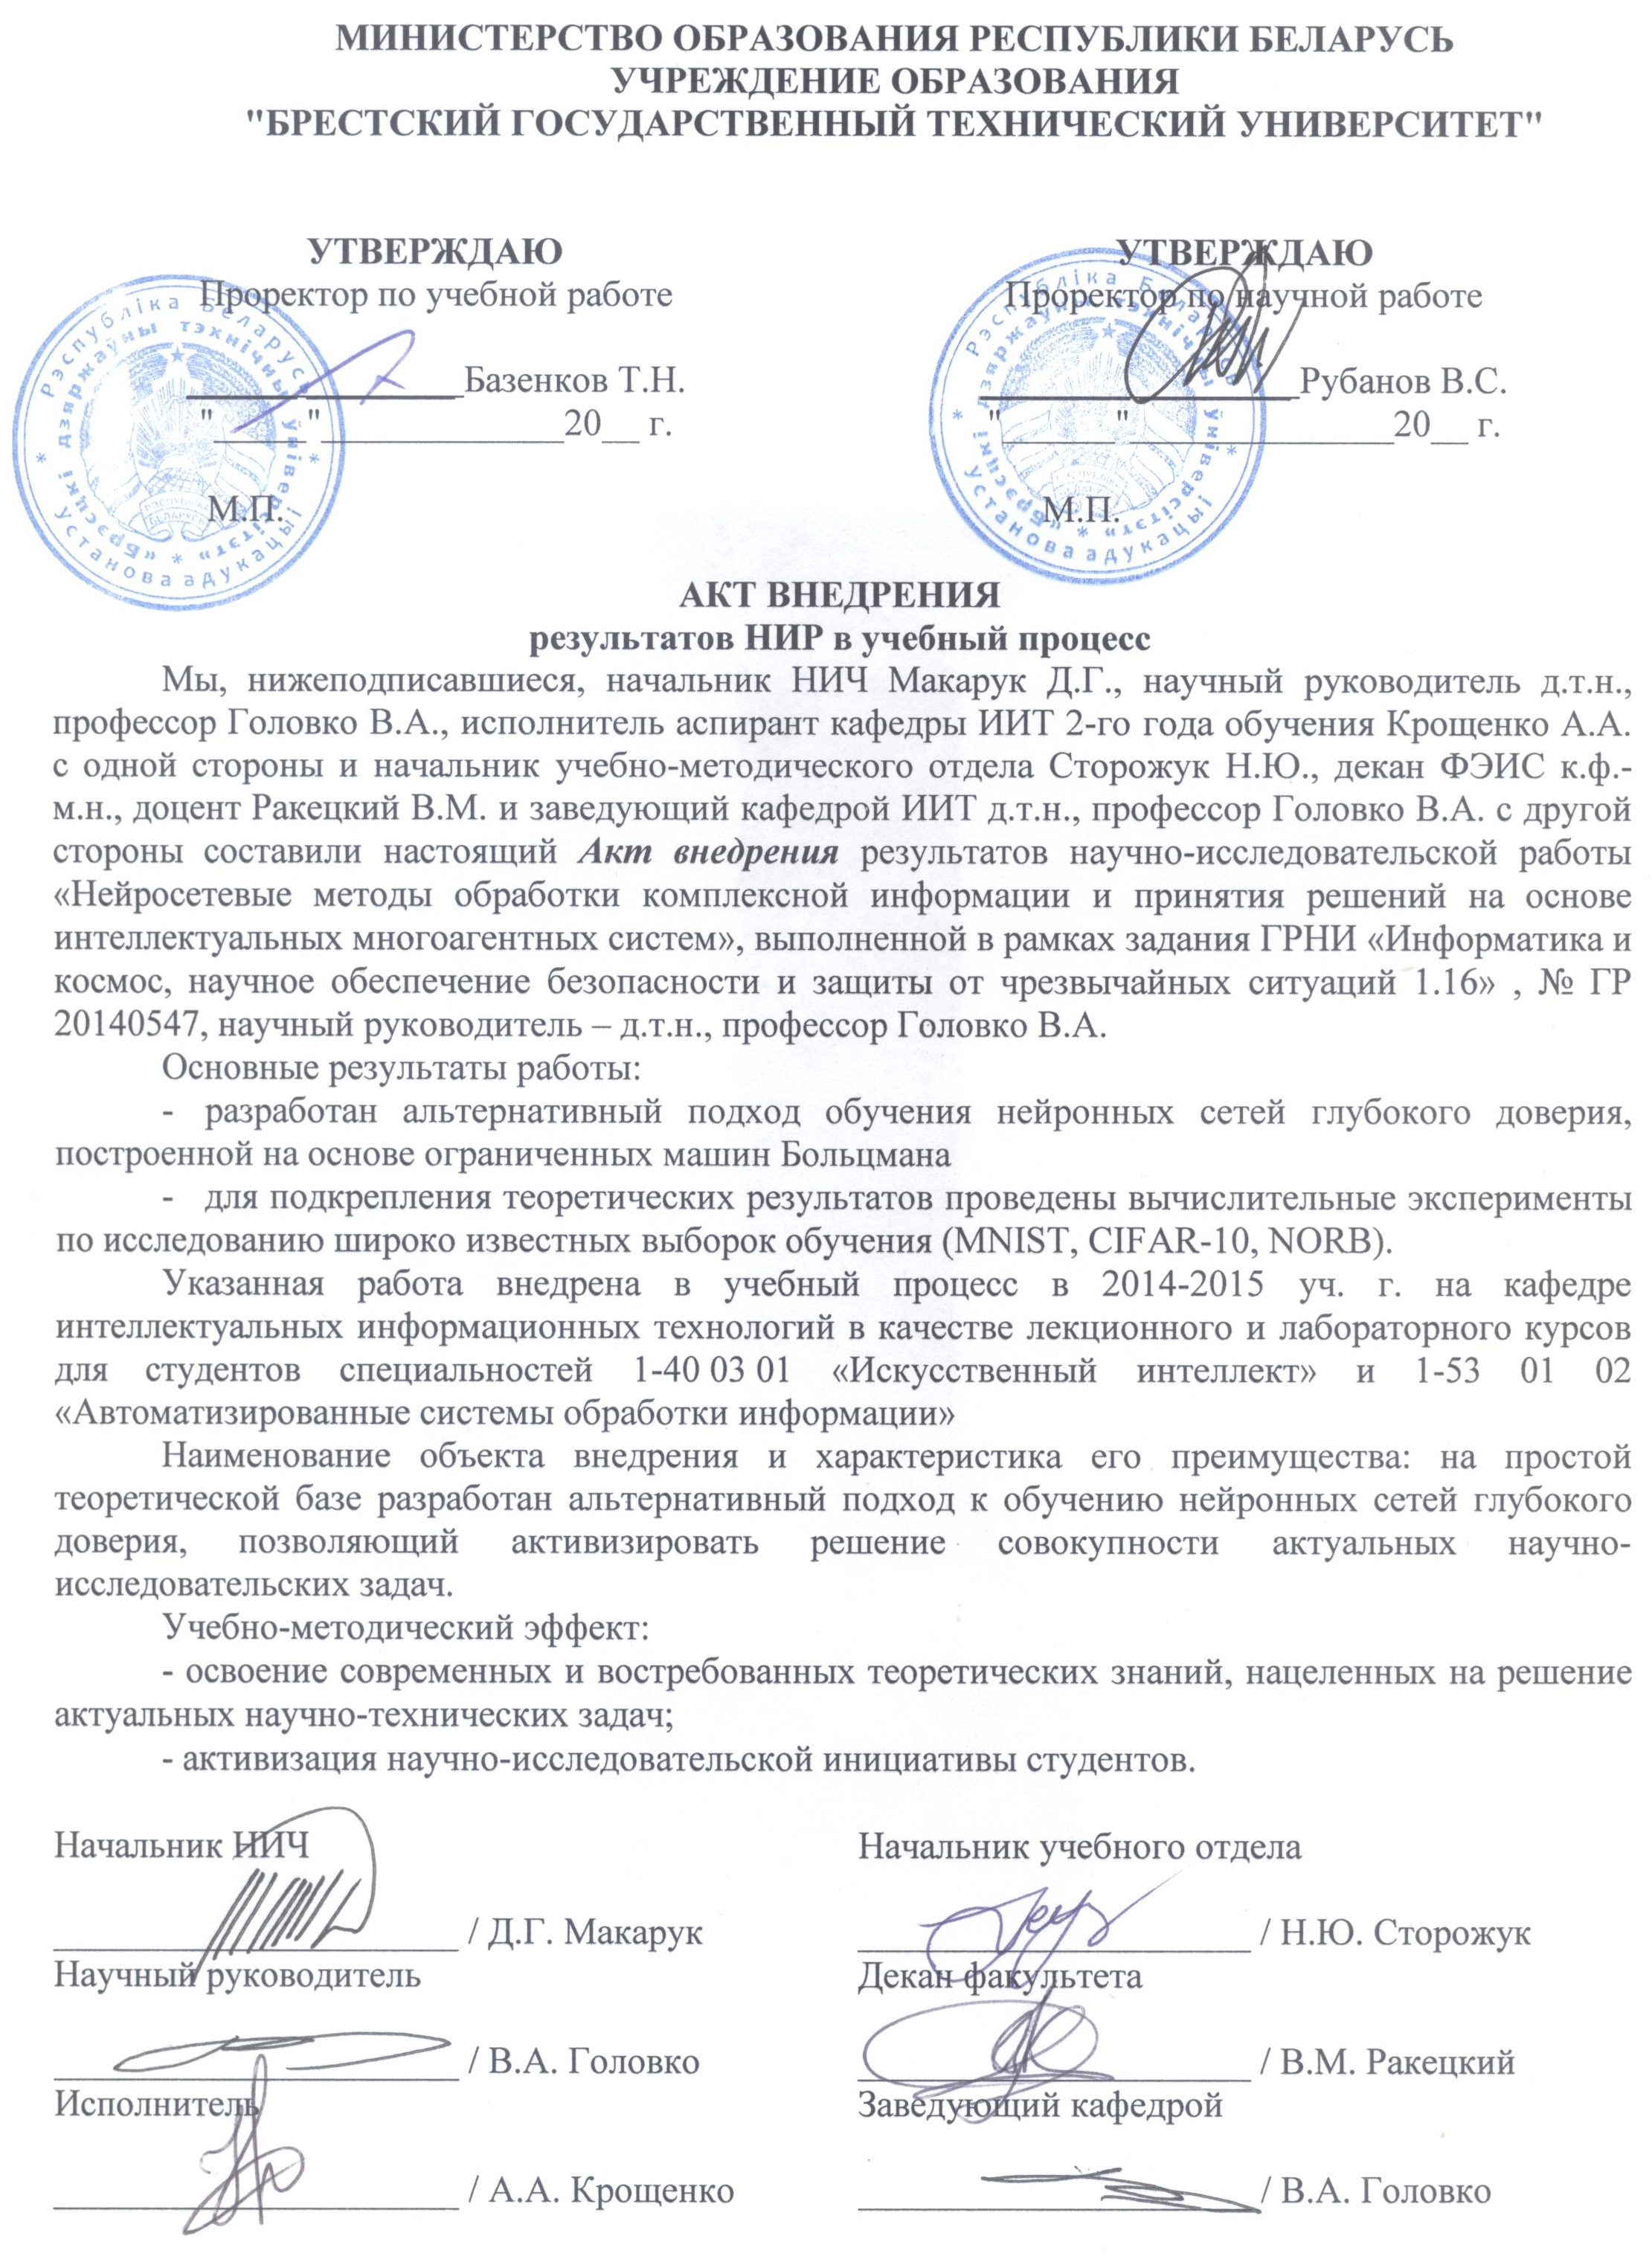
\includegraphics[width=4cm]{actBSTU_1.jpg}
                
\includegraphics[width=4cm]{actISS-2.jpg}
                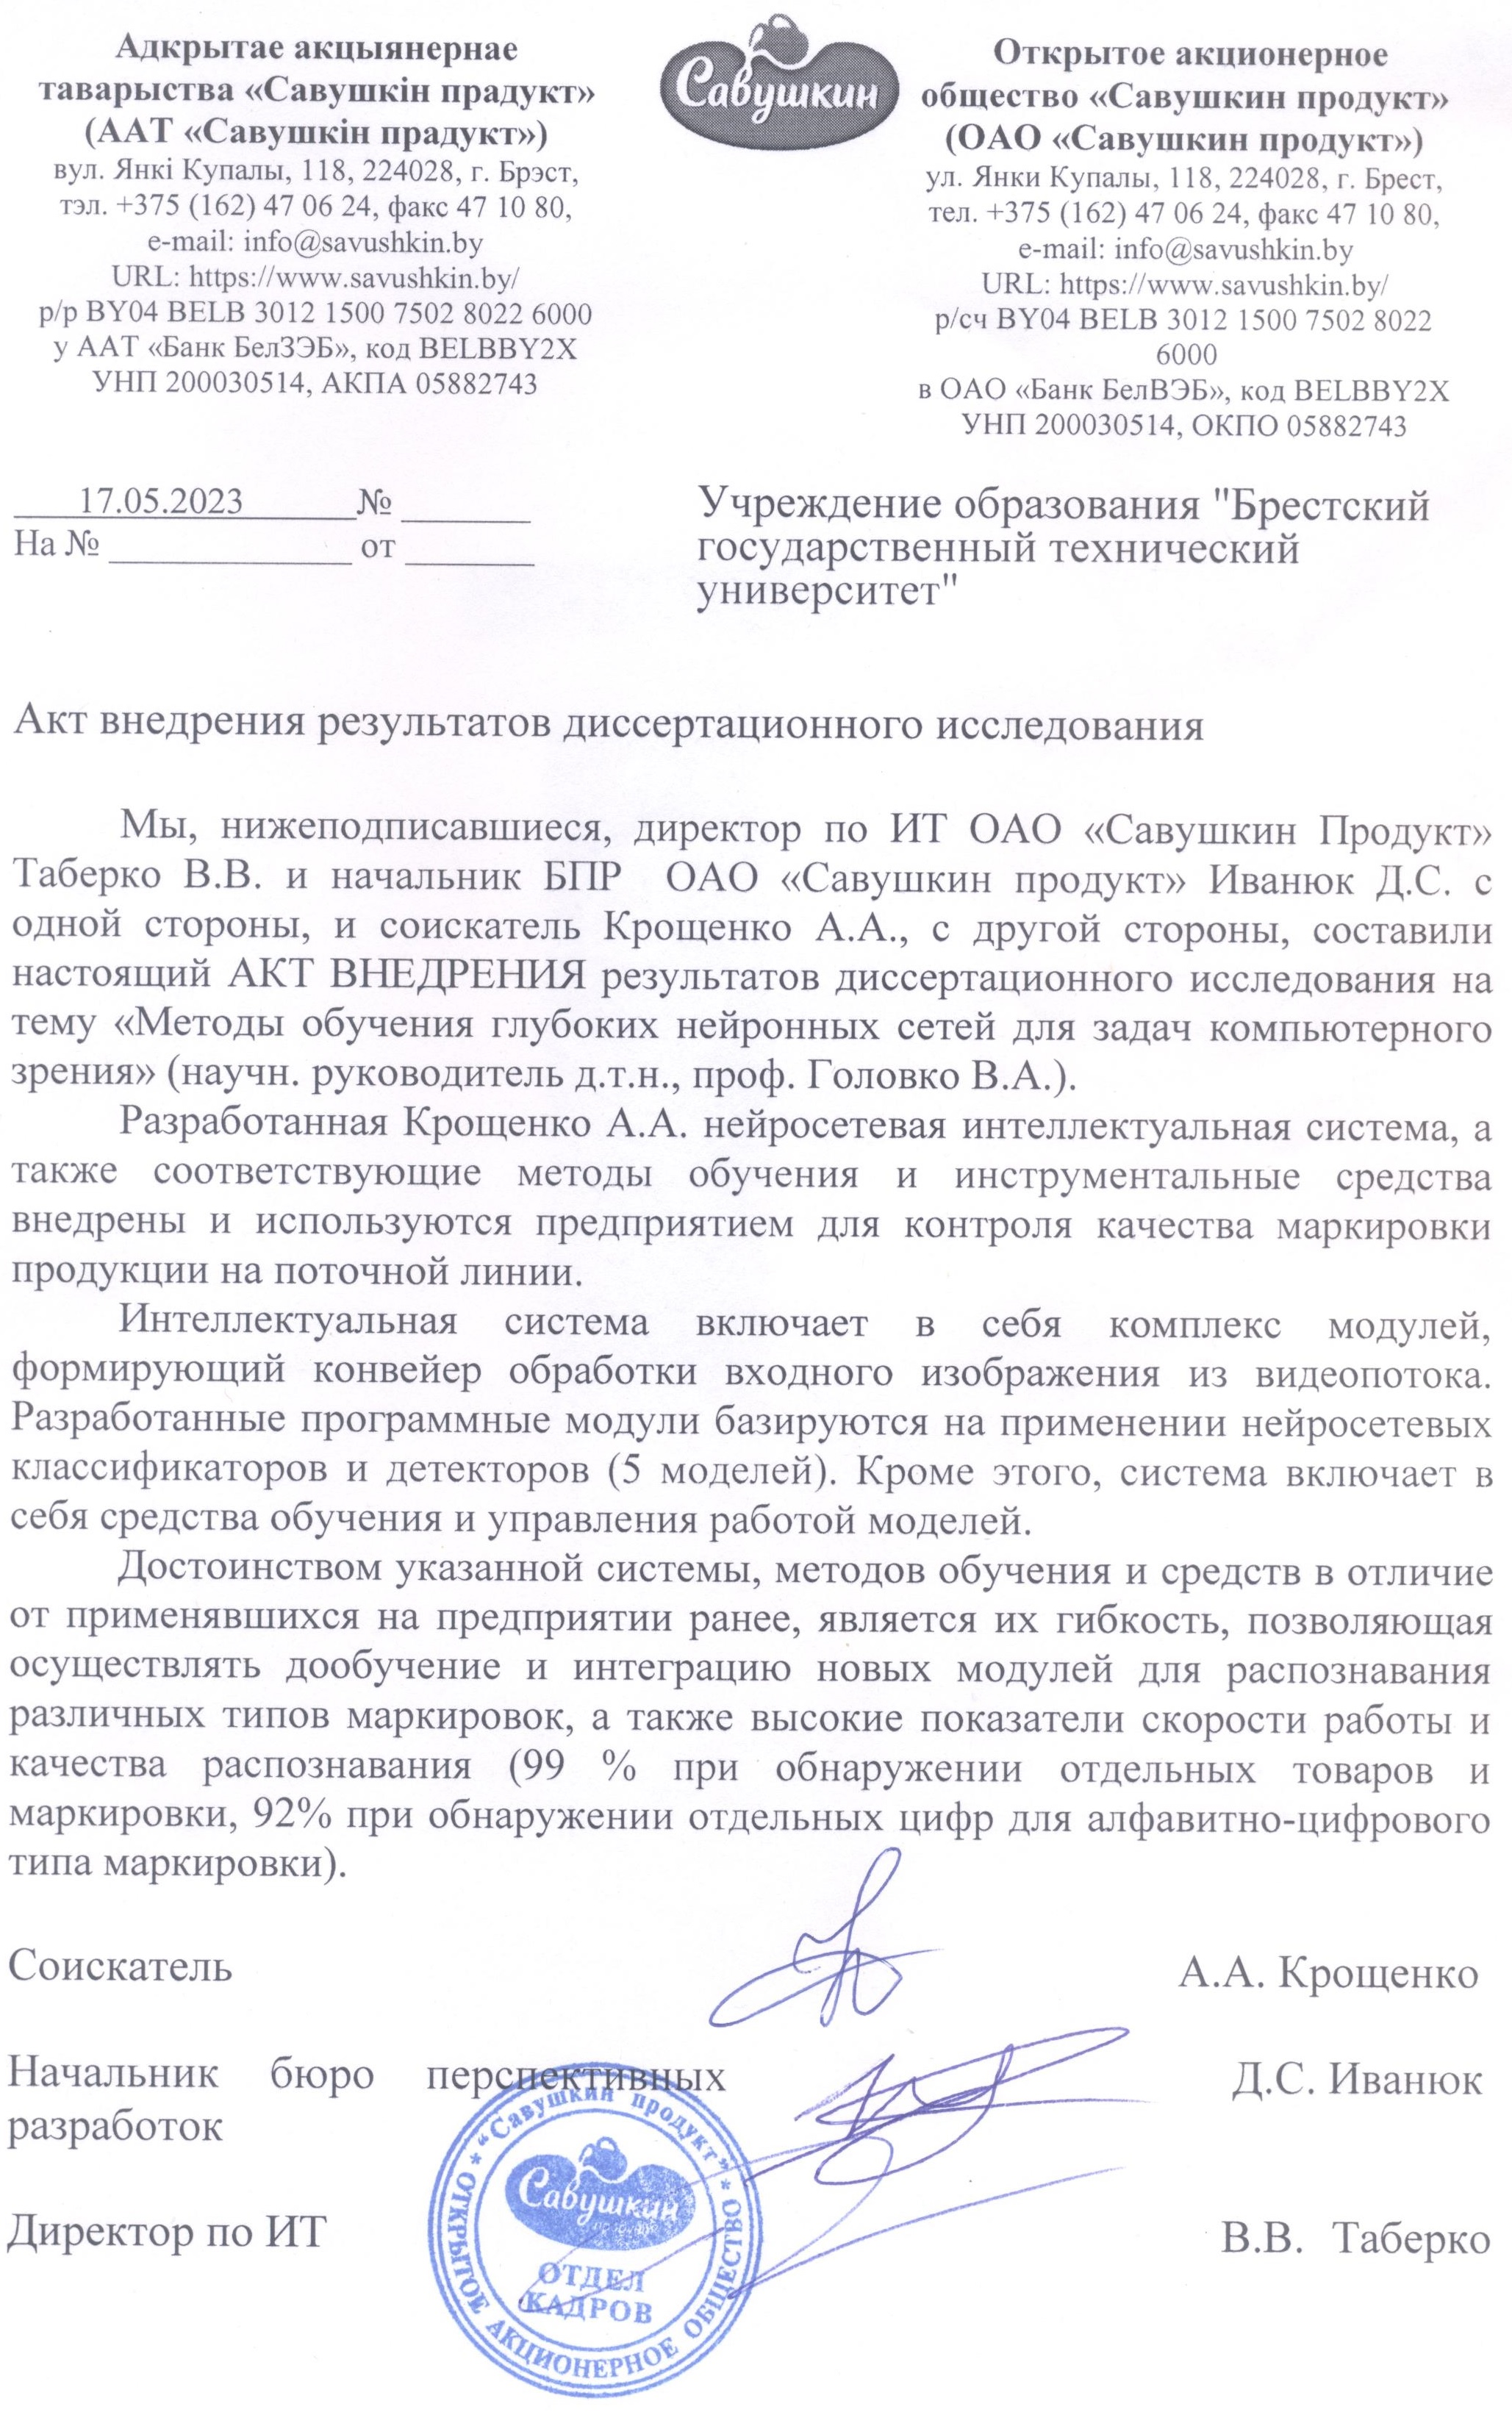
\includegraphics[width=3.5cm]{actSavushkin.jpg}
            \end{minipage}
        \end{figure}
        \end{frame}
	
	% \begin{frame}{Содержание}
	%     \tableofcontents
	% \end{frame}

    % \section{Постановка задачи}
    % \subsection{Общая постановка}
    
    % \begin{frame}{Общая постановка задачи}
    %     Разработать систему проверки корректности нанесения маркировки на продукции ОАО <<Савушкин Продукт>> для различных технологических процессов.
        
    %     В данный момент включает проверку маркировки:
        
    %     \begin{itemize}
    %         \item на самом продукте (например, бутылке);
    %         \item на коробке с готовой продукцией;
    %         \item на поддоне (палете).
    %     \end{itemize}
        
    %     \begin{figure}
    %         \centering
    %         \begin{minipage}[c]{\textwidth}
    %             \centering
    %             \includegraphics[width=3cm]{figures/bottle_line.jpg}
    %             \includegraphics[width=3cm]{figures/robot_sort.jpg}
    %             \includegraphics[width=4cm]{figures/palet.jpg}
    %         \end{minipage}
    %     \end{figure}

    % \end{frame}
    
%     \subsection{Частная постановка}

% 	\begin{frame}
% 		\frametitle{Постановка частной задачи}
		
% 		Разработать систему проверки корректности нанесения маркировки на продукцию (например, бутылки), производимую ОАО ``Савушкин продукт'', на производственной линии
		
% 		\begin{columns}
%             \begin{column}{0.5\textwidth}
%                 \begin{enumerate}
% 		            \item Проверка должна выполняться в реальном времени, основываясь на данных, поступающих с камеры, установленной над производственной линией. Камера формирует видеопоток со скоростью 76 кадров в секунду;
% 		            \item Система должна осуществлять распознавание и проверку как алфавитно-цифрового кода, так и Data Matrix кода и, в будущем, других типов.
%                 \end{enumerate}
%             \end{column}
%             \begin{column}{0.5\textwidth}  %%<--- here
%                 \begin{center}
%                     \includegraphics[width=0.7\textwidth]{figures/bottle_line_camera.jpg}
%                 \end{center}
%             \end{column}
%         \end{columns}
% 	\end{frame}
	
% 	\begin{frame}{Типы маркировок}
% 	    \begin{columns}
%             \begin{column}{0.5\textwidth}
%                 \begin{center}
%                     \begin{figure}
%                         \captionsetup{labelformat=empty} \includegraphics[width=1\textwidth]{figures/digital_code_product.jpg}
%                         \caption{Алфавитно-цифровая маркировка}
%                     \end{figure}
%                 \end{center}
%             \end{column}
%             \begin{column}{0.5\textwidth}  %%<--- here
%                 \begin{center}
%                     \begin{figure}
%                        \captionsetup{labelformat=empty} \includegraphics[width=0.76\textwidth]{figures/box_line.jpg}
                        
%                         \caption{Data Matrix маркировка}
%                     \end{figure}
%                 \end{center}
%             \end{column}
%         \end{columns}
	    
	    
% 	\end{frame}
	
% 	\begin{frame}
% 		\frametitle{Общие подзадачи, решаемые системой}
	
%         Основываясь на постановке задачи, можно выделить следующие общие подзадачи, которые должна решать система: 
%         \begin{enumerate}
%             \item{обнаружение и распознавание типа маркировки;}
%             \item{распознавание маркировки (выделение составных частей и их анализ);}
%             \item{выявление возможных проблем с маркировкой или с процессом.}
%         \end{enumerate}
% 	\end{frame}
	
% \begin{frame}{Диагностируемые проблемы...}
    
%     С маркировкой:
    
%     \begin{enumerate}
%         \item{\textbf{отсутствие:}} в случае поступления на конвейер продуктов без маркировки, система должна сделать вывод об отсутствии чернил, опционально запросив проверку, обратившись к принтеру;
%         \item{\textbf{ошибочность:}} маркировка была обнаружена и распознана, но не совпала с эталонным представлением. В этом случае должен быть сделан вывод о том, что маркировка неверная;
%         \item{\textbf{нечитаемость:}} в случае, если маркировка получается смазанной и не может быть распознана, необходимо остановить конвейер и сообщить об ошибке оператору.
%     \end{enumerate}
    
%     С процессом:
    
%     \begin{enumerate}
%             \item{\textbf{сдвиг камеры:}} если от нейросетевых модулей не поступают данные о результатах распознавания, но системе известно, что движение по конвейеру началось, то она должна сделать вывод о сдвиге камеры.
%     \end{enumerate}
% \end{frame}


% \begin{frame}{... и пути их решения}
    
%     С маркировкой:
    
%     \begin{enumerate}
%         \item{\textbf{отсутствие:}} использование детектора для обнаружения маркировки и продукта -- если продукт найден, а маркировка нет, то сделать \textbf{вывод об отсутствии};
%         \item{\textbf{ошибочность:}} использование детектора для распознавания маркировки -- если итоговый вариант <<собранной>> маркировки отличается от эталона, то сделать \textbf{вывод об ошибочности};
%         \item{\textbf{нечитаемость:}} использование детектора для распознавания маркировки -- если итоговый вариант <<собранной>> маркировки содержит много нераспознанных элементов, сделать \textbf{вывод о нечитаемости};
%     \end{enumerate}
    
%     С процессом:
    
%     \begin{enumerate}
%             \item{\textbf{сдвиг камеры:}} если от нейросетевых модулей не поступают данные о результатах распознавания, но системе известно, что движение по конвейеру началось, то она должна сделать вывод о сдвиге камеры.
%     \end{enumerate}
% \end{frame}

% \subsection{Общие проблемы процесса}
% \begin{frame}{Общие проблемы процесса}
%     \begin{itemize}
%     	\item \textbf{Высокая скорость видеопотока}. Так как скорость видеопотока составляет 76 кадров в секунду, то время обработка каждого кадра составляет около 13 миллисекунд. В тоже время за секунду по конвейеру проходит около 8 единиц продукции (бутылок). Следует отметить, что этого времени недостаточно для запуска сложной нейросетевой архитектуры.
%     	\item \textbf{Невозможность корректной прямой детекции цифр для алфавитно-цифрового типа}. Помимо цифр, содержащихся непосредственно в маркировке, в кадр могут попадать цифры, нанесенные на другие объекты. Помимо этого, следует отметить, что изображение попадает на нейронную сеть с уменьшенным разрешением, что приводит к сложности распознавания мелких объектов (цифр).
%     	\item \textbf{Возможность изменения ориентации маркировки}. В процессе движения товара по производственной линии возможен поворот маркировки на произвольный угол, что приводит к существенному ухудшению распознавания.
%     \end{itemize}
% \end{frame}

% \subsection{Основные требования к системе}
% \begin{frame}{Основные требования к системе}
%     \begin{itemize}
%         \item{\textbf{Высокая скорость работы}. Конвейер движется очень быстро, поэтому обнаружение брака должно осуществляться с минимальными задержками};
%         \item{\textbf{Автономность}. Система должна минимизировать вовлеченность оператора в процесс контроля качества};
%         \item{\textbf{Универсальность}. Система должна настраиваться на распознавание маркировки любой продукции и, в перспективе, любого типа};
%         \item{\textbf{Адаптируемость}. Крайне желательно, чтобы система сохраняла стабильность в работе при любых условиях, возникающих на производстве (например, недостаточность освещения, ошибки персонала и т.д.)}.
%     \end{itemize}
% \end{frame}

% \section{Существующие решения и предлагаемый подход}

% \subsection{Существующие решения}

% \begin{frame}{Применяемые подходы}
%     \begin{itemize}
%         \item Ручная проверка
%         \item Решения на основе датчиков
%     \end{itemize}
    
%     \begin{columns}
%             \begin{column}{0.5\textwidth}
%                 \begin{center}
%                     \begin{figure}
%                         \captionsetup{labelformat=empty} \includegraphics[width=0.6\textwidth]{figures/handly_check.png}
%                     \end{figure}
%                 \end{center}
%             \end{column}
%             \begin{column}{0.5\textwidth}  %%<--- here
%                 \begin{center}
%                     \begin{figure}
%                        \captionsetup{labelformat=empty} \includegraphics[width=0.6\textwidth]{figures/sensor_pictogram.png}
%                     \end{figure}
%                 \end{center}
%             \end{column}
%         \end{columns}
% \end{frame}

% \begin{frame}{Ручная проверка: основные проблемы}

%     \begin{itemize}
%         \item контроль проходит малая часть продукции, таким образом есть вероятность, что дефектная маркировка будет пропущена;
%         \item скорость реакции человека на возникающую нештатную ситуацию может быть недостаточной;
%         \item человек может не заметить небольшое расхождение проверяемой маркировки с эталонной;
%         \item работа по ручной проверке является монотонной.
%     \end{itemize}
% \end{frame}

% \begin{frame}{Имеющиеся решения}
%     Включают решения, базирующиеся на использовании датчиков (например, Omron) и имеют недостатки:
    
%     \begin{itemize}
% 	    \item Нестабильное качество распознавания, зависящее от условий, при которых производится съемка (в частности, от освещенности). Так как производственная линия движется быстро, то необходимые условия для качественного распознавания чаще всего не соблюдаются;
% 	    \item Необходимость покупки специализированного программного обеспечения для настройки датчиков.
%     \end{itemize}
    
%     \textbf{Основной вывод:} системы распознавания на базе датчиков сами нуждаются в контроле
% \end{frame}

% \subsection{Архитектура предлагаемой системы}

% \begin{frame}{Задачи, решаемые архитектурой}
%     \begin{enumerate}
% 	    \item Оценка положения товара
% 	    \item Детекция товара и маркировки
% 	    \item Определение типа маркировки
% 	    \item Поворот маркировки для горизонтальной ориентации
% 	    \item Распознавание маркировки
% 	    \item ``Сборка'' маркировки и ее проверка
%     \end{enumerate}
% \end{frame}

% \begin{frame}{Общая архитектура предлагаемой системы}
%     \begin{figure}[htb]
% 	    \centering
% 	    \includegraphics[width=5.5cm]{figures/savushking_general.png}
%     \end{figure}    
% \end{frame}

% \begin{frame}{Архитектура текущей реализации}
    
%     \begin{figure}[htb]
% 	    \centering
% 	    \includegraphics[width=5.5cm]{figures/savushking_concrete_sheme.png}
%     \end{figure}
% \end{frame}

% \begin{frame}{Представление процесса обработки}
%     \begin{figure}[htb]
% 	    \centering
% 	    \includegraphics[width=2.5cm]{figures/system_work.png}
%     \end{figure}
% \end{frame}

% \subsection{Исходные данные}

% \begin{frame}{Используемые выборки для обучения НС}
%     \begin{itemize}
% 	    \item Выборка для обучения классификатора
% 	    \item Выборка для обучения детектора маркировок и товаров (определения типа маркировки)
% 	    \item Выборка для обучения регрессора угла поворота
% 	    \item Выборка для обучения детектора цифр
%     \end{itemize} 
% \end{frame}

% \begin{frame}{Выборка для обучения детектора маркировок и товаров (определения типа маркировки)}
%     Для формирования этой выборки мы использовали размеченные вручную изображения из выборки для обучения классификатора и дополнительные изображения \textbf{сгенерированных} кодов Data Matrix. Общий объем выборки составил 815 изображений, 163 из которых составили контрольную выборку.
%     \begin{columns}
%             \begin{column}{0.5\textwidth}
%                 \begin{center}
%                     \begin{figure}
%                         \captionsetup{labelformat=empty} \includegraphics[width=0.8\textwidth]{figures/sav_data_matrix_gen.jpg}
%                     \end{figure}
%                 \end{center}
%             \end{column}
%             \begin{column}{0.5\textwidth}  %%<--- here
%                 \begin{center}
%                     \begin{figure}
%                        \captionsetup{labelformat=empty} \includegraphics[width=1\textwidth]{figures/bottle_data_matrix.jpg}
%                     \end{figure}
%                 \end{center}
%             \end{column}
%         \end{columns}
% \end{frame}

% \begin{frame}{Выборка для обучения регрессора угла поворота}
%     При создании данной выборки использовались изображения маркировок, повернутые под произвольными углами. Общий объем выборки составил 59385 изображений, 11877 из которых составили контрольную выборку. В качестве основы брались изображения маркировок, полученных из выборки для обучения детектора маркировок и товаров.
% \end{frame}

% \begin{frame}{Выборка для обучения детектора цифр}
%     Для создания этой выборки применялся датасет номеров домов SVHN, а также размеченные цифровые маркировки. Использовался вариант выборки SVHN, включающий 33.402 изображения в обучающей части и 13.068 в контрольной. Объем выборки размеченных цифровых маркировок составил 419 изображений.
    
%     \begin{figure}[htb]
% 	    \centering
% 	    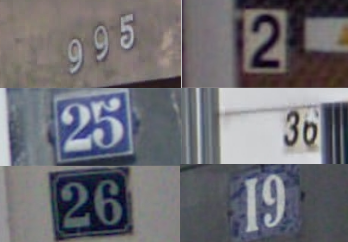
\includegraphics[width=7cm]{figures/svhn.png}
%     \end{figure}
% \end{frame}


% \begin{frame}{Результаты обучения}
%     После обучения классификатора 1 итоговая точность распознавания составила 93.27\%.

%     Применение SSD-модели позволяет достичь эффективности детекции в 99\% (mAP = 0.99) для обнаружения товара и маркировки и 92\% (mAP = 0.92) для отдельных цифр.
    
%     Результаты детекции цифр алфавитно-цифрового кода
%     \begin{center}
        
%     \begin{tabular}{ | c | c |  }
% \hline
% Class label & AP \\ \hline
% 0 & 0.9218\\
% 1. & 0.9107\\
% 2. & 0.9354\\
% 3. & 0.9286\\
% 4. & 0.9265\\
% 5. & 0.9137\\
% 6. & 0.9274\\
% 7. & 0.9167\\
% 8. & 0.9646\\
% 9. & 0.8975\\
% \hline
% \textbf{mAP} & 0.92429\\
% \hline
% \end{tabular}
% \end{center}

% \end{frame}

\begin{frame}
    \centering
    СПАСИБО ЗА ВНИМАНИЕ!
\end{frame}

\end{document}